\documentclass[a4paper, 12pt]{report}
\usepackage[english]{babel}
\usepackage[utf8]{vietnam}

\usepackage{biblatex}
\addbibresource{references.bib}
%\usepackage{vntex}

%\usepackage[english,vietnam]{babel}
%\usepackage[utf8]{inputenc}

%\usepackage[utf8]{inputenc}
%\usepackage[francais]{babel}
\usepackage{a4wide,amssymb,epsfig,latexsym,multicol,array,hhline,fancyhdr}
\usepackage{chngcntr}
\counterwithin{figure}{section}
\counterwithin{table}{section}
\usepackage{amsmath}
\usepackage{lastpage}
\usepackage{abstract}
\usepackage[lined,boxed,commentsnumbered]{algorithm2e}
\usepackage{enumerate}
\usepackage{dirtytalk}
\usepackage{color}
\usepackage[dvipsnames]{xcolor}
\usepackage{tcolorbox}
\usepackage{graphicx}
\usepackage{wrapfig}
\graphicspath{ {figures/} }
% Standard graphics package
\usepackage{listings}
\lstset{frame=tb,
  language=Python,
  aboveskip=3mm,
  belowskip=3mm,
  showstringspaces=false,
  columns=flexible,
  basicstyle={\small\ttfamily},
  numbers=none,
  numberstyle=\tiny\color{gray},
  keywordstyle=\color{blue},
  commentstyle=\color{dkgreen},
  stringstyle=\color{mauve},
  breaklines=true,
  breakatwhitespace=true,
  tabsize=3
}
\definecolor{dkgreen}{rgb}{0,0.6,0}
\definecolor{gray}{rgb}{0.5,0.5,0.5}
\definecolor{mauve}{rgb}{0.58,0,0.82}
\usepackage{array}
\usepackage{tabularx, caption}
\usepackage{multirow}
\usepackage{bm}
\usepackage{multicol}
\usepackage{rotating}
\usepackage{graphics}
\usepackage[a4paper,left=2cm,right=2cm,top=1.8cm,bottom=2.8cm]{geometry}
\usepackage{setspace}
\usepackage{epsfig}
\usepackage{tikz}
\usepackage{diagbox}
\usetikzlibrary{arrows,snakes,backgrounds}
\usepackage[bottom]{footmisc}
\usepackage[unicode]{hyperref}
% \usepackage{indentfirst}
%\usepackage[labelformat=empty]{caption}

%can file puenc.def trong thu muc goc de option [unicode] tao ra bookmark bang tieng Viet
\hypersetup{urlcolor=blue, linkcolor=black, citecolor=green, colorlinks=true} 
%\usepackage{pstcol}                                
% PSTricks with the standard color package

\newtheorem{theorem}{{\bf Theorem}}
\newtheorem{property}{{\bf Property}}
\newtheorem{proposition}{{\bf Proposition}}
\newtheorem{corollary}[proposition]{{\bf Corollary}}
\newtheorem{lemma}[proposition]{{\bf Lemma}}


% \usepackage{fancyhdr}
\setlength{\headheight}{40pt}
\pagestyle{fancy}
\fancyhead{} % clear all header fields
\fancyhead[L]{
 \begin{tabular}{rl}
    \begin{picture}(25,15)(0,0)
    \put(0,-8){
\includegraphics[width=8mm, height=8mm]{hcmut.png}}
    %\put(0,-8){\epsfig{width=10mm,figure=hcmut.eps}}
   \end{picture}&
    %
\includegraphics[width=8mm, height=8mm]{hcmut.png} & %
    \begin{tabular}{l}
        \textbf{\bf \ttfamily Trường Đại học Bách Khoa - Đại học Quốc gia TP.HCM}\\
        \textbf{\bf \ttfamily Bộ môn Viễn Thông}
    \end{tabular}   
 \end{tabular}
}
\fancyhead[R]{
    \begin{tabular}{l}
        \tiny \bf \\
        \tiny \bf 
    \end{tabular}  }

\fancyfoot{} % clear all footer fields
\fancyfoot[L]{\scriptsize \ttfamily Đồ án học kì 202 - 05/2021}
\fancyfoot[R]{\scriptsize \ttfamily {\thepage /vi}}

\renewcommand{\headrulewidth}{0.3pt}
\renewcommand{\footrulewidth}{0.3pt}

\fancypagestyle{plain}{%
\fancyhead{} % clear all header fields
\fancyhead[L]{
 \begin{tabular}{rl}
    \begin{picture}(25,15)(0,0)
    \put(0,-8){
\includegraphics[width=8mm, height=8mm]{hcmut.png}}
    %\put(0,-8){\epsfig{width=10mm,figure=hcmut.eps}}
   \end{picture}&
    %
\includegraphics[width=8mm, height=8mm]{hcmut.png} & %
    \begin{tabular}{l}
        \textbf{\bf \ttfamily Trường Đại học Bách Khoa - Đại học Quốc gia TP.HCM}\\
        \textbf{\bf \ttfamily Bộ môn Viễn Thông}
    \end{tabular}   
 \end{tabular}
}
\fancyhead[R]{
    \begin{tabular}{l}
        \tiny \bf \\
        \tiny \bf 
    \end{tabular}  }

\fancyfoot{} % clear all footer fields
\fancyfoot[L]{\scriptsize \ttfamily Đồ án học kì 202 - 05/2021}
\fancyfoot[R]{\scriptsize \ttfamily {\thepage /vi}}

\renewcommand{\headrulewidth}{0.3pt}
\renewcommand{\footrulewidth}{0.3pt}}

%%%
\setcounter{secnumdepth}{4}
\setcounter{tocdepth}{3}
\makeatletter
\newcounter {subsubsubsection}[subsubsection]
\renewcommand\thesubsubsubsection{\thesubsubsection .\@alph\c@subsubsubsection}
\newcommand\subsubsubsection{\@startsection{subsubsubsection}{4}{\z@}%
                                     {-3.25ex\@plus -1ex \@minus -.2ex}%
                                     {1.5ex \@plus .2ex}%
                                     {\normalfont\normalsize\bfseries}}
\newcommand*\l@subsubsubsection{\@dottedtocline{3}{10.0em}{4.1em}}
\newcommand*{\subsubsubsectionmark}[1]{}
\makeatother

\begin{document}

\begin{titlepage}

\begin{center}
TRƯỜNG ĐẠI HỌC BÁCH KHOA - ĐẠI HỌC QUỐC GIA TP.HCM\\
BỘ MÔN VIỄN THÔNG
\end{center}

\vspace{1cm}

\begin{figure}[!h]
\begin{center}

\includegraphics[width=5cm]{hcmut.png}
\end{center}
\end{figure}

\vspace{1cm}


\begin{center}
\begin{tabular}{c}
\multicolumn{1}{l}{\textbf{{\Large ĐỒ ÁN HỌC KÌ 202}}}\\
~~\\
\hline
\\
\textbf{\Huge Tạo màu cho ảnh xám sử dụng}\\
\textbf{\Huge mạng đối nghịch tạo sinh có điều kiện}\\
\\
\hline
\end{tabular}
\end{center}

\vspace{3cm}

\begin{table}[h]
\begin{tabular}{rrl}

\hspace{2cm} & GVHD: PGS.TS. Hà Hoàng Kha & (hhkha@hcmut.edu.vn)\\
& Sinh viên: & Nguyễn Thành Trung - 1814515\\
& & (trung.nguyendx@hcmut.edu.vn)\\
\vspace{30pt}\\

\end{tabular}
\end{table}

\begin{center}
{\footnotesize Hồ Chí Minh, 05/2021}
\end{center}
\end{titlepage}


%\thispagestyle{empty}
\pagenumbering{roman}

\renewcommand{\abstractnamefont}{\normalfont\Huge\bfseries}

\renewcommand{\abstractname}{Lời cảm ơn}
\begin{abstract}
 Trước tiên, em muốn bày tỏ lòng biết ơn chân thành tới giáo viên hướng dẫn của em, thầy \textbf{PGS.TS Hà Hoàng Kha} - ``giảng viên bộ môn Viễn Thông khoa Điện--Điện Tử'' đã trực tiếp giúp đỡ, hướng dẫn và cho lời khuyên trong việc nghiên cứu, thực hiện, chỉnh sửa và hoàn thiện đồ án.\vspace{5pt}

Em cũng muốn gửi lời cảm ơn chân thành đến trường \textbf{Đại học Bách Khoa TP.HCM - Đại học Quốc gia TP.HCM}, khoa \textbf{Điện-Điện Tử}, bộ môn \textbf{Viễn Thông} đã cung cấp những kiến thức nền tảng, cách thức học tập và nghiên cứu.
Thật khó để tưởng tượng rằng em sẽ tiếp cận và xử lý đề tài đồ án như thế nào nếu không có những vốn liếng quý báu đó.\vspace{5pt}

Cũng không thể quên cảm ơn một số anh khoá trên cùng các bạn cùng khoá và một vài cá nhân đã giúp đỡ em rất nhiều trong quá trình tìm hiểu đề tài cũng như thực hiện khảo sát lấy số liệu cho đánh giá kết quả của đồ án.\vspace{5pt}

Em xin chân thành cảm ơn tất cả.\vspace{20pt}\\

\hfill
\begin{tabular}{l@{}}
\textit{Tp. Hồ Chí Minh, ngày \textbf{04} tháng \textbf{05} năm \textbf{2021}.}\vspace{10pt}\\
\hspace{3cm}\textbf{Sinh Viên}
\end{tabular} 
\end{abstract}

\renewcommand{\abstractname}{Tóm tắt nội dung đồ án}
\begin{abstract}
Tạo màu cho ảnh xám là một chủ đề nóng hổi và thú vị trong ngành thị giác máy tính trong khoảng hai thập kỉ vừa qua.
Rất nhiều những nghiên cứu đã được thực hiện và cho rất nhiều phương pháp với những kết quả ấn tượng.
Tuy việc tạo màu cho mỗi trường hợp là một bài toán có không ít lời giải vì rất nhiều màu có thể có cùng mức xám.
Dẫn đến việc, với một tấm ảnh xám đầu vào, ta có thể có nhiều phương án màu lựa chọn mà vẫn có được tính chân thực.
Nhưng điều đó không đồng nghĩa với việc đây là một bài toán đơn giản mà trái lại là một vấn đề nan giải.\vspace{5pt}

Trong đồ án này, hai mô hình mạng đối nghịch tạo sinh có điều kiện - cGAN có bộ sinh kiến trúc Unet xây dựng bằng xương sống chuyển giao từ mạng phân loại ResNet18 và bộ phân biệt kiến trúc PatchGAN $70\times 70$, được triển khai và huấn luyện với tập dữ liệu COCO để xử lý vấn đề này.
Chất lượng mô hình đầu tiên thông qua một cuộc khảo sát thực tế 100 người với thang điểm từ 1 (rất giả) đến 5 (rất thật).
Mô hình thứ hai là mô hình được cải thiện bằng cách đưa ra thay đổi nhỏ trong hàm mất và tăng số lượng dữ liệu huấn luyện.
Chất lượng của hai mô hình được so sánh định tính qua những kết quả thử nghiệm, cũng như định lượng qua hai giá trị MSE và RMSE của mỗi mô hình.\vspace{5pt}

Bên cạnh đó, xây dựng một API tạo màu bằng khung phần mềm Django của Python, từ đó triển khai một ứng dụng web đơn giản để tạo màu cho ảnh bằng khung phần mềm VueJS của Javascript.
\end{abstract}

\tableofcontents

\newpage

% \thispagestyle{empty}
\renewcommand{\listfigurename}{Danh sách hình}
\listoffigures

\newpage

% \thispagestyle{empty}
% \renewcommand{\listfigurename}{Danh sách hình minh hoạ}
\listoftables

%%%%%%%%%%%%%%%%%%%%%%%%%%%%%%%%%
\chapter*{Danh sách quy ước ký hiệu và tên gọi được sử dụng trong đồ án}

\begin{center}
\begin{tabular}{c|l}
    $x, y, M, N$ & các số vô hướng, hoặc là một biến tổng quát tuỳ từng trường hợp\\
    $\mathbf{x}, \mathbf{y}$ & các vector cột\\
    $\mathbf{X}, \mathbf{Y}$ & các ma trận, hoặc tensor tuỳ tường trường hợp\\
    $\bm{X}, \bm{Y}$ & các tập hợp\\
    $\bm{X}^{M \times N}$ & tập hợp các ma trận kích thước $M$ hàng, $N$ cột với các phần tử thuộc tập $\bm{X}$\\
    $\mathbb{N}^*$ & tập hợp các số tự nhiên khác $0$\\
    $\mathbb{R}$ & tập hợp các số thực\\
    $\mathbb{R}^n$ & tập hợp các vector $n$ chiều với các phần tử thuộc tập $\mathbb{R}$\\
    $\{x, y\}$ & tập hợp chứa các phần tử $x$, $y$\\
    $[x, y]$ & tập hợp $\{x, x + 1, \dots, y - 1, y\}$\\
    $(x, y)$ & tập hợp $[x, y]$ bỏ đi phần tử $x$ và $y$, hoặc toạ độ vị trí tuỳ từng trường hợp\\
    $\left|\bm{X}\right|$ & số phần tử của tập $\bm{X}$\\
    $\sim$ & tương đương, thuộc về\\
    $xy, x \times y$ & tích của hai vô hướng\\
    $x / y, \dfrac{x}{y}$ & thương của hai vô hướng, $x$ chia $y$\\
    $\lfloor x \rfloor$ & làm tròn xuống của $x$\\
    $\sum_{i=1}^nx_i$ & tổng của $x_1 + x_2 + \dots + x_n$\\
    $\mathbf{O}_{m \times n}$ & ma trận kích thước $m$ hàng $n$ cột với tất cả các phần tử bằng $0$\\
    $\mathbf{J}_{m \times n}$ & ma trận kích thước $m$ hàng $n$ cột với tất cả các phần tử bằng $1$\\
    $\bm{X} \times \bm{Y}$ & tích Descartes của tập $\bm{X}$ và $\bm{Y}$\\
    $\prod_{i=1}^n\bm{X}_i$ & tích Descartes của $n$ tập\\
    $\mathcal{G}, f, g$ & ánh xạ, hàm số\\
    $\mathcal{I}$ & ảnh số\\
    $\mathcal{I}^{\left(c\right)}$ & kênh $c$ của ảnh số\\
    $\displaystyle \arg\min_xf$ & giá trị của $x$ để hàm số $f$ đạt giá trị nhỏ nhất.\\
    $\displaystyle \arg\max_xf$ & giá trị của $x$ để hàm số $f$ đạt giá trị lớn nhất.\\
    $e$ & hằng số Euler - hằng số Napier\\
    $\log\left(\cdot\right)$ & hàm logarit cơ số $e$\\
    $\mathbb{E}\left\{\cdot\right\}$ & kỳ vọng toán\\
    $\widehat{\left(\cdot\right)}$ & giá trị dự đoán của mô hình\\
    $\left(\cdot\right)_{ij}, \left(\cdot\right)_{i, j}$ & tất cả các giá trị của ma trận hoặc tensor ở toạ độ $(i, j)$\\
    & lấy trong từng không gian bỏ đi 2 chiều sâu nhất\\
    $\left(\cdot\right)_{i:i + m, j:j + n}$ & tất cả các giá trị của ma trận hoặc tensor ở các toạ độ $[i, i + m] \times [j, j + n]$\\
    & lấy trong từng không gian bỏ đi 2 chiều sâu nhất\\
\end{tabular}
\end{center}

% \newpage
% \vspace*{\fill}
% {\centering \textit{Trang này được cố ý để trống.}\par}
% \vspace{\fill}

\newpage

\pagenumbering{arabic}
\fancyfoot{} % clear all footer fields
\fancyfoot[L]{\scriptsize \ttfamily Đồ án học kì 202 - 05/2021}
% \fancyfoot[R]{\scriptsize \ttfamily {\thepage /vi}}
\fancyfoot[R]{\scriptsize \ttfamily {\thepage}/\pageref{LastPage}}

\fancypagestyle{plain}{%
\fancyfoot{} % clear all footer fields
\fancyfoot[L]{\scriptsize \ttfamily Đồ án học kì 202 - 05/2021}
% \fancyfoot[R]{\scriptsize \ttfamily {\thepage /vi}}
\fancyfoot[R]{\scriptsize \ttfamily {\thepage}/\pageref{LastPage}}}

%%%%%%%%%%%%%%%%%%%%%%%%%%%%%%%%%
\chapter{Giới thiệu}

\section{Tổng quan}\label{overview}

Nhu cầu phục chế ảnh màu từ ảnh xám (đen trắng) không phải là hiếm.
Thông thường là ảnh do tác động của thời gian làm mất hoặc sai màu.
Đôi khi lại là ảnh được chụp ở thời xưa, thời đại chưa có công nghệ chụp ảnh màu.
Và vì nhiều mục đích cho việc trải nghiệm chân thực, con người chúng ta muốn tái tạo lại màu cho những hình ảnh chưa có màu đó.\vspace{5pt}

Hiện nay, hầu hết những người thợ chỉnh sửa ảnh đều sử dụng phương pháp thủ công để phục hồi màu.
Tuy có sự giúp đỡ của các công cụ hỗ trợ như các phần mềm thao tác với ảnh trên máy tính, để có thể có một tấm ảnh đẹp cũng đòi hỏi mất nhiều thời gian \cite{replytime2colorize2012}.
Đôi khi có thể lên đến một hoặc hai tháng đối với những bức ảnh có nhiều chi tiết phức tạp.\vspace{5pt}

Ở góc nhìn kỹ thuật, phục chế màu, hay tạo màu cho ảnh xám là một bài toán phức tạp có nhiều lời giải, vì việc một đối tượng trong một bức ảnh có thể có nhiều màu thích hợp.
Chẳng hạn như một nải chuối có thể màu lục khi chưa chín nhưng lại cũng có thể là màu vàng khi chín, và thậm chí có thể đã chín nhưng vẫn còn màu lục (hình \ref{fig:banana}).
Do đó, việc khôi phục lại đúng chính xác màu cho một bức ảnh bất kì là chuyện gần như bất khả thi và cũng không cần thiết.
Nhưng cũng không vì thế mà ta có thể gán một màu bất kì cho một đối tượng nào đó, giả sử như việc màu da người là màu xanh biển hoặc mặt trời là màu xanh lá.
Nhìn một tấm ảnh sau khi được khôi phục màu lại có màu không phù hợp, phản ánh không khớp với những gì chúng ta quan sát thường ngày, hiển nhiên không phải là mục đích để chúng ta phải cực khổ đi khôi phục màu.\vspace{5pt}

\begin{wrapfigure}{l}{0pt}
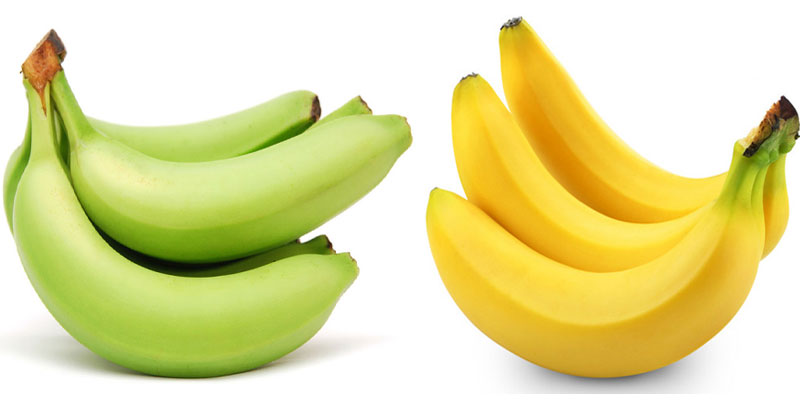
\includegraphics[width=10.7cm]{images/1_1.jpg} 
\caption{Nải chuối có thể màu lục hoặc màu vàng.}
\label{fig:banana}
\end{wrapfigure}


Trước khi có sự xuất hiện của ngành học máy/học sâu \cite{wikiml2021, wikideeplearning2021} trong việc xử lý ảnh, đã có rất nhiều kỹ thuật được đưa ra cho quá trình tự động phục hồi màu cho ảnh xám [\textbf{\ref{scribblemethods}}, \textbf{\ref{examplarmethods}}].
Nhưng để có được một kết quả ưng ý, đều hoặc nhiều hoặc ít dựa vào sự can thiệp của bàn tay con người.
Sau khi học sâu bùng nổ trong ngành thị giác máy tính, rất nhiều mô hình học sâu ứng dụng mạng tích chập [\textbf{\ref{convolutionnet}}] đã có thể học và tạo ra màu cho những ảnh xám [\textbf{\ref{deeplearningmethods}}, \textbf{\ref{enhancemodel}}] (hình \ref{fig:deoldify}).

\section{Mục tiêu}\label{objective}

Theo những gì đã nghiên cứu về đề tài [\textbf{\ref{overview}}], đồ án này được đưa ra với mục đích xây dựng và huấn luyện một mô hình mạng học sâu để tạo màu cho ảnh xám.
Yêu cầu của màu tạo ra không nhất thiết phải giống hoàn toàn so với màu thực (màu của ảnh/vật gốc nếu có).
Thay vào đó là độ chân thực, hợp lí của ảnh sau khi ảnh được kết hợp với màu được tạo sẽ là thứ được hướng đến.
Mức độ chân thực, hợp lí sẽ được đánh giá định tính bằng một cuộc khảo sát trực tuyến gồm 100 người tham gia [\textbf{\ref{surveyforevaluation}}], và một chút định lượng thông qua hai giá trị MSE và RMSE [\textbf{\ref{mseandrmseeval}}]\vspace{5pt}

Các nội dung trong đồ án sẽ được trình bày từ những cơ sở lý thuyết để giải quyết bài toán tạo màu.
Từ những khái niệm nền tảng về ảnh số, cho tới kiến trúc mô hình được sử dụng.
Tiếp theo là phần triển khai và huấn luyện mô hình.
Sau đó là đánh giá, cải thiện mô hình và so sánh, rồi ứng dụng mô hình vừa hoàn thành.
Cuối cùng là tổng kết và nêu ra hướng phát triển cho đề tài đồ án.
Trong các nội dung được trình bày, những phần chính yếu, cần nhiều sự quan tâm hơn cả sẽ là:

\begin{itemize}
    \item Lựa chọn không gian màu thích hợp để sử dụng cho bài toán tạo màu [\textbf{\ref{reasontopicklab}}].
    \item Mạng đối nghịch tạo sinh [\textbf{\ref{ganarchitecture}}].
    \item Mạnh tích chập Unet [\textbf{\ref{unetarchitecture}}].
    \item Kiến trúc khung mô hình mạng học sâu pix2pix [\textbf{\ref{pix2pixarchitecture}}].
    \item Kiến Mô hình mạng học sâu xử lý bài toán tạo màu dựa vào kiến trúc pix2pix [\textbf{\ref{mainarchitecture}}].
    \item Triển khai mô hình sử dụng ngôn ngữ lập trình Python và thư viện Pytorch [\textbf{\ref{implementation}}].
    \item Đánh giá, cải thiện mô hình và so sánh [\textbf{\ref{testmodel}}].
\end{itemize}

\begin{figure}[!h]
\captionsetup{width=0.8\textwidth}
\centering
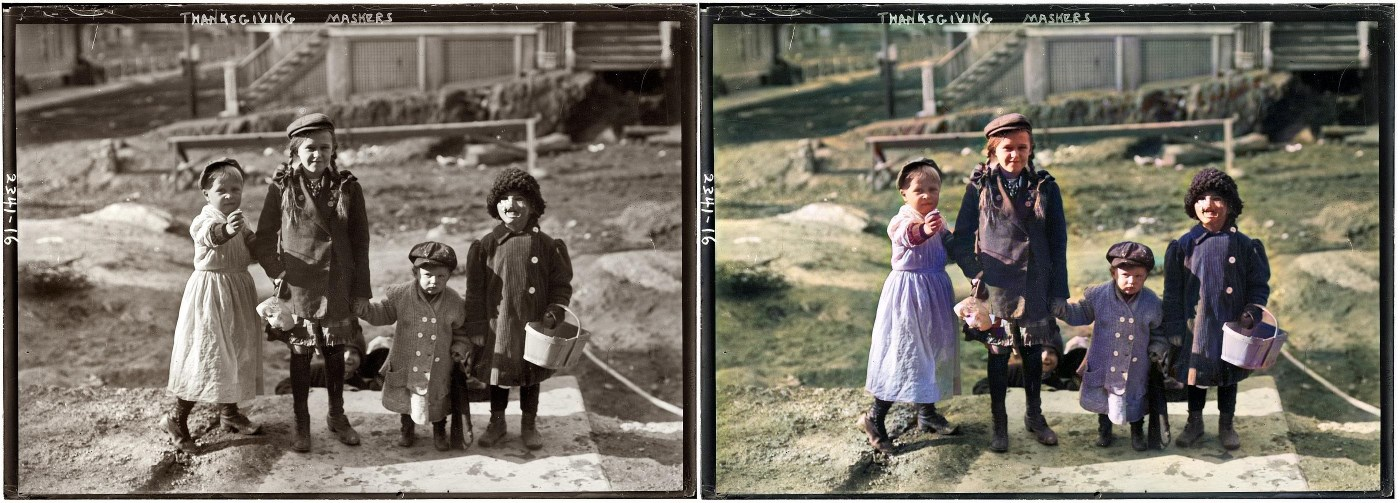
\includegraphics[width=15cm]{images/thanksgiving.jpg}
\caption{Hình ảnh ngày lễ tạ ơn được chụp năm 1911, được tái tạo màu bằng DeOldify - một dự án học sâu \cite{deoldify2020, deoldifyreddit2012}.}
\label{fig:deoldify}
\end{figure}

%%%%%%%%%%%%%%%%%%%%%%%%%%%%%%%%%

\chapter{Cở sở lý thuyết về ảnh số và các không gian màu}

\section{Giới thiệu cơ bản về ảnh số}\label{intro2ditimg}

\begin{wrapfigure}{r}{0pt}
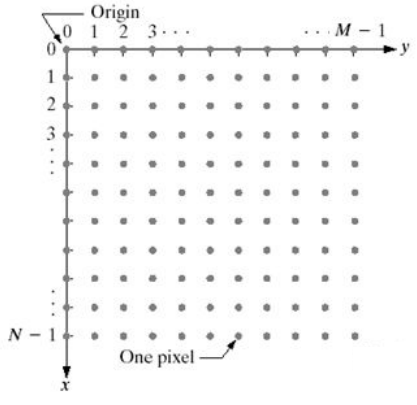
\includegraphics[width=8.7cm]{images/pxy.PNG} 
\caption{Không gian toạ độ của ảnh số.}
\label{fig:pxy}
\end{wrapfigure}

Máy tính là một công cụ rất mạnh mẽ để xử lý những vấn đề của con người.
Nhưng chúng bị hạn chế khi chỉ xử lý dữ liệu dưới dạng các con số.
Hình ảnh cũng không phải ngoại lệ.
Ảnh số - ảnh mà máy tính hiểu, thực tế là tập hợp hữu hạn các điểm ảnh dưới dạng một ma trận 2 chiều $\mathcal{I} \in \bm{G}^{W\times H}; \bm{G} = \prod_{i=1}^{C}\bm{G}_i$.
Trong đó , $W \in \mathbb{N}^*$ và $H \in \mathbb{N}^*$ lần lượt là chiều rộng và chiều cao của ảnh được tính bằng đơn vị điểm ảnh \cite{introtocvnttuan}.
Mỗi điểm ảnh $p_{xy} \in \bm{G}$ là một phần tử của ảnh tại toạ độ nguyên $(x, y); 0 \le x \le H - 1, 0 \le y \le  W - 1$ (hình \ref{fig:pxy}, $H=N, W=M$), có giá trị trong một tập hữu hạn $\left(\left|\bm{G}\right| \neq \infty\right)$, biểu thị cho mức xám hoặc màu nhất định của nó.
Mức xám hoặc màu nhất định được biểu diễn như thế nào tuỳ thuộc vào loại ảnh số: \textbf{ảnh nhị phân}, \textbf{ảnh xám (đen trắng)} [\textbf{\ref{grayimage}}] hay \textbf{ảnh màu} [\textbf{\ref{colorfulimage}}].

\section{Ảnh nhị phân và ảnh xám}\label{grayimage}

Ảnh nhị phân \cite{wikibinimg2021} là loại ảnh sơ khai và đơn giản nhất.
Mỗi điểm ảnh $p_{xy} \in \bm{G}_{\text{nhị phân}} = \{0, 1\}$ được biểu diễn bằng 1 bit.
Với $p_{xy} = 0$ thì điểm ảnh nhận màu đen, và ngược lại thì sẽ nhận màu trắng (hình \ref{fig:binimg}).\vspace{5pt}

Khác một chút so với ảnh nhị phân, ảnh xám \cite{wikigrayimg2021} có tập giá trị đa dạng hơn là $\bm{G}_{\text{xám}} = [0, 255]$, được biểu diễn bằng 1 byte (8 bit).
Cũng như ảnh nhị phân, giá trị điểm ảnh càng lớn thì màu của điểm ảnh đó càng gần màu trắng.
Nhờ có nhiều mức màu hơn so với ảnh nhị phân (hình \ref{fig:grayscale}), ảnh xám cho ra những hình ảnh đẹp hơn.

\begin{figure}[!h]
\captionsetup{width=0.8\textwidth}
\centering
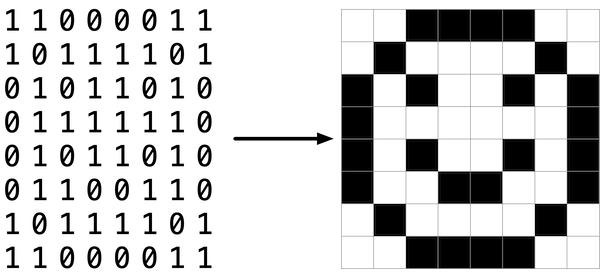
\includegraphics[width=10cm]{images/binimg.png}
\caption{Ảnh nhị phân $8\times 8$ và biểu diễn ma trận của nó.}
\label{fig:binimg}
\end{figure}

\begin{figure}[!h]
\captionsetup{width=0.8\textwidth}
\centering
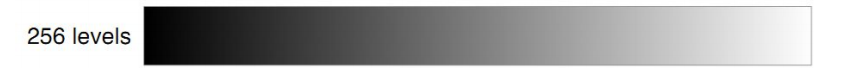
\includegraphics[width=14cm]{images/grayscale.PNG}
\caption{256 mức màu của ảnh xám.}
\label{fig:grayscale}
\end{figure}

\section{Ảnh màu và một số không gian màu cho ảnh màu}\label{colorfulimage}

Khi nói về một con số là tốc độ của một vật, ta có thể tưởng tượng theo nhiều hướng khác nhau.
Giả sử con số ta đang đề cập là $40$.
Nếu như ta chạy xe máy trong thành phố, thì tốc độ $40$ ki-lô-mét/giờ là một vận tốc được cho phép.
Nhưng nếu nó là $40$ dặm/giờ ($\approx 64.3738$ ki-lô-mét/giờ), thì ta cũng có thể bị bắn tốc độ ngay cả khi là ở ngoài khu vực đông dân cư.
Còn nếu là $40$ mét/giây ($=144$ ki-lô-mét/giờ), chắc chỉ có thể thấy vận tốc này ở trong các trường đua xe.\vspace{5pt}

Rõ ràng, khi nói tới vận tốc, con số là phần quan trọng.
Nhưng đồng thời, đơn vị biểu diễn là điều buộc phải có.
Ảnh màu cũng vậy, sẽ là khá thiếu xót nếu ta cần xử lý sâu một tấm ảnh nhưng không biết được ảnh đang được xử lý đang thuộc không gian màu nào.
Vì không tồn tại duy nhất một không gian màu \cite{wikicolorspace2021} cho mọi loại ảnh.
Điều này là do nhu cầu và mục đích của con người rất đa dạng, dẫn tới có nhiều loại không gian màu đã được tạo ra để đáp ứng.\vspace{5pt}

Các không gian biểu diễn ảnh màu đều có nhiều hơn 1 kênh so với ảnh nhị phân và ảnh xám, và thường là $C=3$ kênh giá trị để biểu diễn cho một điểm ảnh $\left(p_{xy} \in \bm{G}_{1}\times \bm{G}_{2}\times \bm{G}_{3}\right)$.
Giống với ảnh xám, mỗi kênh màu đều sử dụng 1 byte số nguyên.
Trong đồ án này, để tiện lưu trữ và xử lý, giá trị trong mỗi điểm ảnh sẽ được tách riêng thành $C$ ma trận kích thước $W\times H$, xếp chồng thành một tensor\footnote{Wikipedia, ``Tensor'', \href{https://en.wikipedia.org/wiki/Tensor}{https://en.wikipedia.org/wiki/Tensor}} có số chiều $C\times W \times H$ [\textbf{\ref{convolutionnet}}, \textbf{\ref{implementation}}].

\subsection{Không gian màu RGB}

Hầu hết khi làm việc với ảnh số, ta sẽ thao tác với ảnh có không gian màu là \textbf{RGB} \cite{wikirgb2021}, ảnh có 3 kênh màu đỏ-lục-lam (hình \ref{fig:inspectrgb}) $\left(\bm{G}_{\text{RGB}} = \bm{G}_{\text{R}}\times \bm{G}_{\text{G}}\times \bm{G}_{\text{B}}\right)$.
Đây cũng là không gian màu phổ biến với đại đa số mọi người và được sử dụng rộng rãi hiện nay.
Các kênh màu $\bm{G}_{\text{R}}, \bm{G}_{\text{G}}, \bm{G}_{\text{B}}$ của không gian màu \textbf{RGB} có giá trị nằm trong đoạn $[0, 255]$.\vspace{5pt}

\begin{figure}[!h]
\captionsetup{width=0.8\textwidth}
\centering

\includegraphics[width=4cm]{images/rgbmodel.png}
\caption{Phối trộn màu bổ sung.}
\label{fig:rgbmodel}
\end{figure}

\begin{figure}[!h]
\captionsetup{width=0.8\textwidth}
\centering
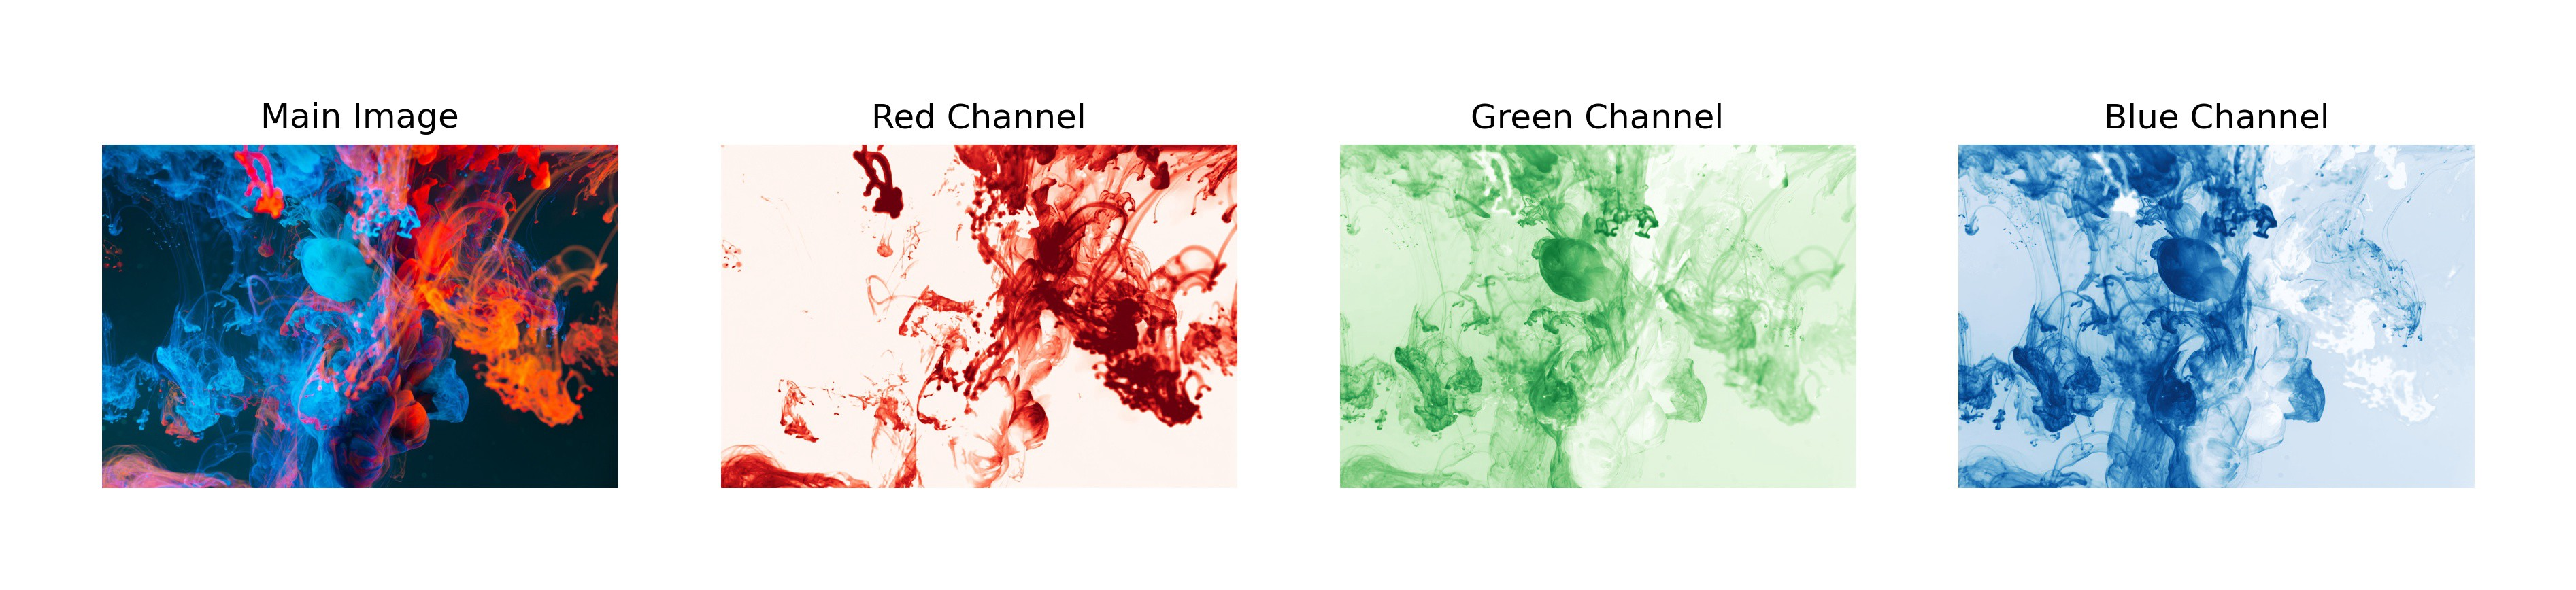
\includegraphics[width=16cm]{images/2_1.jpeg}
\caption{Các kênh màu đỏ, lục và lam được tách ra riêng biệt \cite{moeincolorization2020}.}
\label{fig:inspectrgb}
\end{figure}

Chỉ với 3 màu đỏ, lục và lam, nhưng ta lại có thể tạo ra được khoảng hơn 16 triệu (chính xác là $256^3$) màu khác nhau.
Trong đó, 7 màu chủ đạo là đỏ, lục, lam, trắng, vàng, xanh ngọc, và hồng (hình \ref{fig:rgbmodel}).
Thêm đỏ vào xanh lá cây tạo ra vàng.
Thêm vàng vào xanh lam tạo ra trắng.
Sự kỳ diệu này có được dựa trên cơ sở phản ứng sinh lý học của mắt người với ánh sáng \cite{wikirgb2021}.\vspace{5pt}

Với nhu cầu hình ảnh ghép, đã xuất hiện phương án thêm vào 1 kênh 8 bit cho độ trong suốt.
Kênh trong suốt được biết đến với tên là \textit{alpha}, vì thế, nên định dạng này có tên là \textbf{RGBA} \cite{wikirgba2021}. Cũng lưu ý rằng, vì nó không thay đổi bất kỳ cái gì trong mô hình \textbf{RGB}, nên \textbf{RGBA} không phải là một mô hình màu khác biệt.
Nó chỉ là định dạng bổ sung thêm thông tin về độ trong suốt cùng với thông tin màu.

\subsection{Không gian màu L*a*b*}\label{introtolabspace}

\begin{wrapfigure}{l}{0pt}
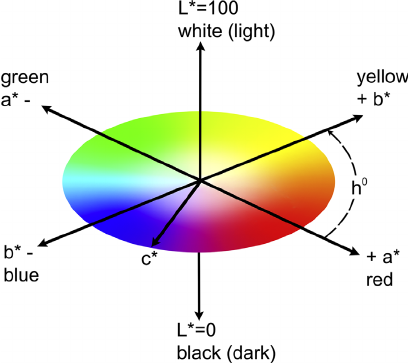
\includegraphics[width=8cm]{images/2_2.png} 
\caption{Không gian màu Lab.}
\label{fig:labspace}
\end{wrapfigure}

Ngoài \textbf{RGB}, một không gian màu khác cũng được sử dụng khá nhiều là không gian màu \textbf{L*a*b*} \cite{wikilab2021} - hệ màu được xây dựng dựa trên khả năng cảm nhận của mắt người.
Các giá trị của \textbf{L*a*b*} mô tả tất cả những màu mà mắt người bình thường có thể nhìn thấy được.
Mô hình màu này được xem là độc lập với thiết bị và thường được sử dụng như một cơ sở tham chiếu khi chuyển đổi từ một không gian màu này sang một không gian màu khác.\vspace{5pt}

Cũng như \textbf{RGB}, Không gian \textbf{L*a*b*} cũng quan tấm đến 3 thông số của mỗi điểm ảnh (hình \ref{fig:inspectlab}) $\left(\bm{G}_{\mathbf{L^*}\mathbf{a^*}\mathbf{b^*}} = \bm{G}_{\mathbf{L}^*} \times \bm{G}_{\mathbf{a}^*} \times \bm{G}_{\mathbf{b}^*}\right)$.
Thông số đầu tiên là \textbf{L*} đại diện cho độ sáng của của mỗi điểm ảnh.
Giá trị \textbf{L*} càng lớn thì điểm ảnh càng nghiêng về màu trắng, ngược lại thì sẽ là màu đen.
Hai thông số còn lại là \textbf{a*} và \textbf{b*} sẽ mang thông tin lần lượt là lục-đỏ và vàng-lam.
Giá trị \textbf{a*} càng thấp thì điểm ảnh nghiêng về lục nhiều, đỏ ít.
Ngược lại thì lục ít, đỏ nhiều và tương tự với giá trị \textbf{b*}.
Theo mô hình \textbf{L*a*b*}, tất cả các màu có cùng độ sáng \textbf{L*} sẽ cùng nằm trên một mặt phẳng có dạng hình tròn theo 2 trục \textbf{a*} và \textbf{b*} (hình \ref{fig:labspace}).\vspace{5pt}

Giá trị của kênh \textbf{L*} nằm trong tập $\mathbf{G}_{\mathbf{L}^*} = [0, 100]$.
Về phần 2 kênh còn lại là \textbf{a*} và \textbf{b*}, không có cụ thể một khoảng nhất định mà tuỳ thuộc vào phần mềm, chương trình mà ta sử dụng.
Nhưng thông thường sẽ là $\mathbf{G}_{\mathbf{a}^*} \times \mathbf{G}_{\mathbf{b}^*} = [-128, 127] \times [-128, 127]$.

\begin{figure}[!h]
\captionsetup{width=0.8\textwidth}
\centering
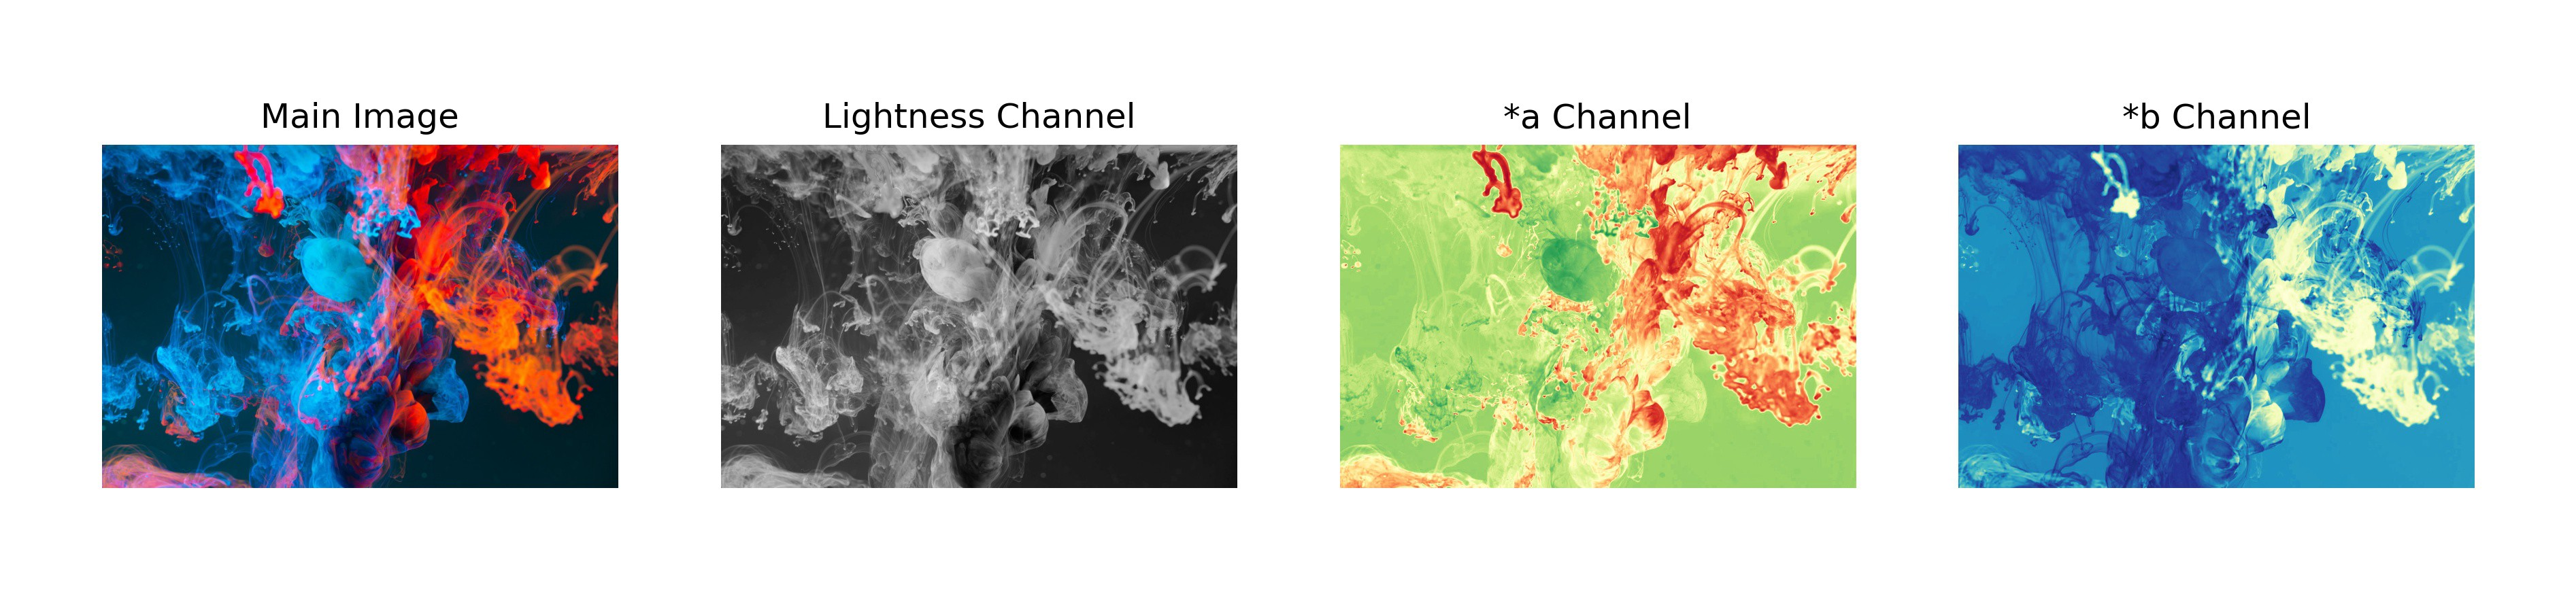
\includegraphics[width=16cm]{images/2_3.jpeg}
\caption{Các giá trị \textbf{L}, \textbf{a} và \textbf{b} được tách ra riêng biệt \cite{moeincolorization2020}.}
\label{fig:inspectlab}
\end{figure}

\subsection{Lợi thế trong bài toán tạo màu của không gian màu L*a*b* so với không gian màu RGB}\label{reasontopicklab}

Ngoài hai không gian màu \textbf{RGB} và \textbf{L*a*b*}, còn một số không gian màu khác như \textbf{CMYK} \cite{wikicmyk2021}, \textbf{HSV} \cite{wikihsv2021},... Vậy nên, lựa chọn một không gian màu thích hợp để xử lý một bài toán cũng là một vấn đề cần đắn đo.\vspace{5pt}

Giữa hai không gian màu \textbf{RGB} và \textbf{L*a*b*}, mặc dù \textbf{RGB} có sự phổ biến nhiều hơn, nó vẫn không được lựa chọn để xử lý cho bài toán tạo màu. Sẽ có hai lợi thế khi sử dụng \textbf{L*a*b*} thay vì \textbf{RGB}:

\begin{enumerate}[i)]
    \item Không gian màu \textbf{L*a*b*} được thiết kế để đồng nhất về cảm giác về màu sắc của con người, điều này làm cho không gian màu này trở nên lý tưởng cho việc xử lý máy tính.
    \item Tận dụng kênh mức xám đầu vào để làm kênh độ sáng \textbf{L*} bằng cách điều chỉnh tỉ lệ. Khi đó mô hình chỉ phải dự đoán 2 kênh \textbf{a*} và \textbf{b*} thay vì phải dự đoán 3 kênh trong không gian \textbf{RGB}.\label{enum:secondreason}
\end{enumerate}

Trong hai lợi thế được nêu ra, (\ref{enum:secondreason}) được cho là lý do chính mà không gian màu \textbf{L*a*b*} trở thành không gian trong đại đa số các bài toán tạo màu cho ảnh xám.
Và trong đồ án này, cũng không phải là một trường hợp ngoại lệ, không gian màu sử dụng để xử lý bài toán sẽ là không gian \textbf{L*a*b*}.

\chapter{Những phương pháp đã được đề xuất cho bài toán tạo màu}\label{proposedmethods}

Trong khoảng hai thập kỷ vừa qua, rất nhiều phương pháp đã được đề xuất.
Chúng có thể được chia ra làm 3 loại phương pháp chính: \textbf{đánh dấu màu một vài điểm ảnh rồi dùng thuật toán loang}, \textbf{dựa vào mẫu có bố cục tương tự} và cuối cùng là phương pháp \textbf{học sâu}.
Hai loại phương pháp đầu tiên chưa phải là một phương pháp hoàn toàn tự động, mà vẫn phải cần có sự can thiệp từ con người.
Phương pháp thứ 3 là sử dụng học sâu thì hoàn toàn tự động, khi mô hình học sâu có thể học được màu tương ứng của các đối tượng từ những dữ liệu huấn luyện.

\section{Phương pháp đánh dấu màu một vài điểm ảnh rồi dùng thuật toán loang}\label{scribblemethods}

Được đề xuất bởi Levin \cite{alevincolorization}, từ một tấm ảnh xám đầu vào, ta sẽ vẽ một vài màu cơ bản từ đó làm nền tảng, định hướng cho mô hình.
Ý tưởng này xuất phát từ quan sát rằng, những điểm ảnh có độ sáng gần bằng nhau (mức xám xấp xỉ) và có khoảng cách trên ảnh gần nhau sẽ có khả năng tương tự cao dẫn đến màu giống nhau.\vspace{5pt}

Một vài cách cải thiện độ hiệu quả của phương pháp trên như là sử dụng thông tin các cạnh để thuật toán loang hoạt động chính xác hơn \cite{huangcolorization}.
Hay theo như Luan \cite{luancolorization}, ta sẽ đánh dấu mỗi màu cho mỗi phân đoạn khác nhau (hình \ref{fig:scribblemethod}). 

\begin{figure}[!h]
\captionsetup{width=0.8\textwidth}
\centering
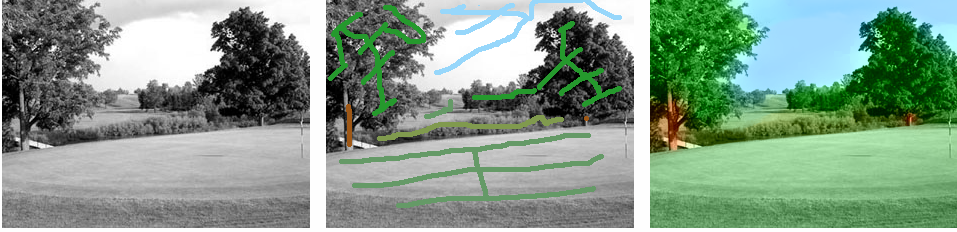
\includegraphics[width=15cm]{images/2_4.png}
\caption{Mô tả ý tưởng thuật toán đánh dấu vài điểm ảnh \cite{trungcolorization2018}.}
\label{fig:scribblemethod}
\end{figure}

Phương pháp thuộc loại này nhìn chung có kết quả màu rất tốt, nhưng lại đòi hỏi không ít sức người.
Đặc biệt với những ảnh nhiều chi tiết thì, việc đánh dấu màu sẽ trở nên khó khăn và tốn nhiều thời gian.
Thêm nữa, việc chọn màu để đánh dấu cũng không phải là một vấn đề dễ dàng với một người có ít kinh nghiệm về màu sắc.

\section{Phương pháp dựa vào mẫu}\label{examplarmethods}

Đây là một loại phương pháp sử dụng một mẫu giống hoặc tương tự để giải quyết bài toán.
Welsh \cite{welshcolorization} khởi xướng phương pháp này bằng cách dựa vào màu của ảnh có bố cục tương tự (hình \ref{fig:examplarmethod}).
Ta chọn ra một tấm ảnh mẫu có bố cục tương tự rồi dựa vào màu của ảnh mẫu, kết hợp chỉnh sửa để đưa ra dự đoán.
Một vấn đề gặp phải khi ta sử dụng phương pháp trên đó là sự gắn kết không gian đã gần như bị bỏ qua.
Để khắc phục, Ironi \cite{ironicolorization} đề xuất việc đưa màu của những phân đoạn của ảnh mẫu sang dùng để đánh dấu màu rồi dùng thuật toán loang [\textbf{\ref{scribblemethods}}].
Một hướng khác, Tai \cite{taicolorization} xây dựng xác suất từng phân đoạn của cả hai bức hình, sau đó chuyển màu từ ảnh mẫu sang ảnh cần tạo màu theo những vùng có kết quả thống kê gần tương xứng.

\begin{figure}[!h]
\captionsetup{width=0.8\textwidth}
\centering
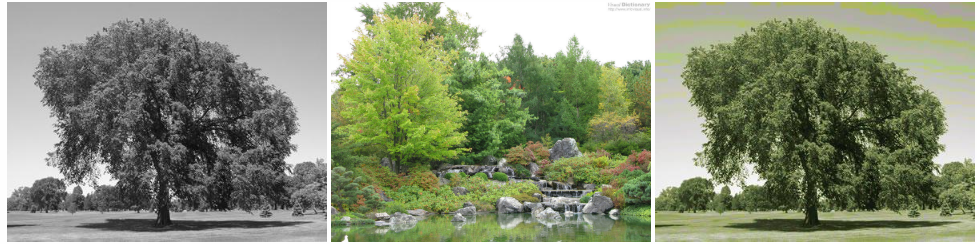
\includegraphics[width=15cm]{images/2_5.png}
\caption{Mô tả ý tưởng thuật toán ảnh có bố cục tương tự \cite{trungcolorization2018}.}
\label{fig:examplarmethod}
\end{figure}


Dù loại phương pháp này đã giảm thiểu được phần nhiều tính thủ công, nhưng lại bị phụ thuộc lớn vào ảnh mẫu, ảnh mà phải có bố cục tương tự so với ảnh cần xử lý.

\section{Phương pháp học sâu}\label{deeplearningmethods}

Sau này, bằng cách tận dụng những cặp ảnh (xám, màu), rất nhiều phương pháp dựa vào học sâu đã được ra đời.
Đầu tiên nhất là Cheng \cite{chengcolorization}, khi triển khai một mô hình mạng nơ-ron sâu hoàn toàn tự động tạo màu, thông qua việc xây dựng và tối ưu bài toán bình phương tối thiểu, với đầu vào của mô hình là bộ những mô tả ngữ cảnh.
Nổi tiếng và thành công nhất trong phương pháp loại này có thể nói đến là Zhang \cite{zhangcolorization}, bằng việc học phân phối màu của mỗi điểm ảnh.
Mô hình của Zhang được huấn luyện với đa thức entropy chéo kết hợp việc cân bằng các lớp hiếm để tạo ra được những màu ít xuất hiện.\vspace{5pt}

Riêng với những phương pháp học sâu đời đầu như Cheng có thể cải tiến dựa vào những nghiên cứu về mạng tích chập.
Về sau, khi tập dữ liệu để huấn luyện trở nên lớn thì những mô hình học sâu gần như đã có thể tự động tô màu một cách cực kì chân thật, không thua gì so với kết quả được làm thủ công bởi những người thợ chỉnh sửa ảnh lâu năm.
Và có thể đánh lừa mắt người xem giữa ảnh gốc và ảnh được tô màu.\vspace{5pt}

Đồ án này trình bày một phương pháp học sâu, với mô hình học sâu ứng dụng khung mô hình mạng học sâu \textbf{pix2pix} được đề xuất bởi Isola \cite{isola2018imagetoimage}.
Khung mô hình sử dụng mạng \textbf{GAN} \cite{goodfellow2014generative} có điều kiện với bộ sinh có kiến trúc mạng \textbf{Unet} \cite{ronneberger2015unet} kết hợp với bộ phân biệt Patch.

\chapter{Khung mô hình mạng học sâu pix2pix}\label{pix2pixframework}

Với mong muốn có một cái nhìn rõ ràng về kiến trúc mô hình được áp dụng cho bài toán tạo màu của đồ án này, sẽ là không hề lãng phí nếu ta dành một chút thời gian để đi qua những thành phần chính của khung mô hình pix2pix.\vspace{5pt}

Nòng cốt của khung là một mạng đối nghịch tạo sinh GAN [\textbf{\ref{ganarchitecture}}] với một sinh theo kiến trúc mạng Unet [\textbf{\ref{unetarchitecture}}].
Những đặc điểm khác biệt của mạng GAN trong khung mô hình so với mạng GAN thông thường cũng sẽ được trình bày [\textbf{\ref{overviewofpix2pix}}].
Như việc tạo nhiễu, hay điều kiện đầu vào của bộ phân biệt.
Ngoài ra, bộ phân biệt có kiến trúc Patch cũng sẽ được đề cập [\textbf{\ref{patchdiscriminator}}].

\section{Mạng đối nghịch tạo sinh (GAN - Generative Adversarial Network)}\label{ganarchitecture}

Yann LeCun, giám đốc Facebook AI Research, từng nhận xét về ý tưởng của mạng GAN:

\say{The most interesting idea in the last 10 years in Machine Learning.}

Tạm dịch:

\say{Là ý tưởng thú ví nhất về Học Máy trong vòng 10 năm qua.}\vspace{5pt}

Những lời có cánh từ một trong những người có tầm ảnh hưởng trong ngành khoa học máy tính, quả là một điều tuyệt vời.
Và thật vậy, GAN đã có được rất nhiều thành tựu từ khi được giới thiệu với công chúng từ năm 2014 bởi Ian J.Goodfellow và công sự của mình \cite{goodfellow2014generative}.

\subsection{Khái quát về mạng GAN}\label{gannetwork}

\begin{figure}[!h]
\captionsetup{width=0.8\textwidth}
\centering
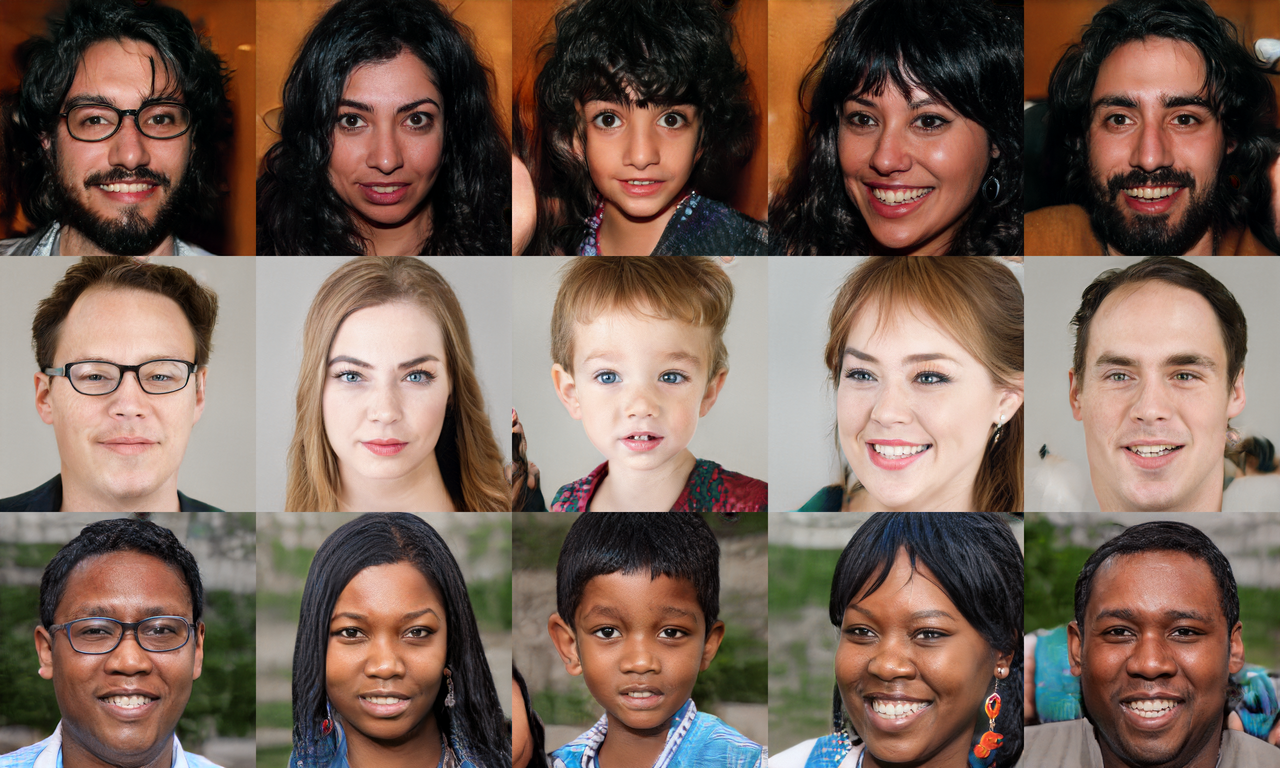
\includegraphics[width=15cm]{images/2_6.PNG}
\caption{Ảnh mặt người sinh ra bởi StyleGAN \cite{karras2019stylebased}.}
\label{fig:facesstylegan}
\end{figure}

Mạng GAN thuộc nhóm mô hình sinh dữ liệu mới.
Dữ liệu sinh ra nhìn như thật nhưng không phải thật.
Ví dụ như ảnh mặt người (hình \ref{fig:facesstylegan}) là do GAN sinh ra, không phải mặt người thật.\vspace{5pt}

G - \textbf{G}enerative ý chỉ sinh, N - \textbf{N}etwork là mạng, còn A - \textbf{A}dversarial là đối nghịch.
Lí do đối nghịch là trong mạng này được tạo nên từ sự kết hợp giữa 2 mạng là \textbf{bộ sinh} ($G$ \textit{- \textbf{G}enerator}) và \textbf{bộ phân biệt} (\textit{D - \textbf{D}iscriminator}), luôn luôn đối nghịch nhau trong quá trình huấn luyện.
Trong khi bộ sinh cố gắng sinh ra các dữ liệu giống như thật thì bộ phân biệt lại cố gắng phân biệt đâu là dữ liệu được sinh ra từ bộ sinh và đâu là dữ liệu thật.\vspace{5pt}

Giả sử như bài toán đưa cho GAN là sinh ra tiền giả giống như tiền thật để có thể dùng được (hình \ref{fig:thiefandpolice}), thì bộ sinh là người làm tiền giả, còn bộ phân biệt giống như cảnh sát.
Người làm tiền giả sẽ cố gắng làm ra những tờ tiền giả làm sao để cảnh sát không biết đó là giả, còn cảnh sát thì cố gắng học để phân biệt được tiền nào là giả, tiền nào là thật.

\begin{figure}[!h]
\captionsetup{width=0.8\textwidth}
\centering
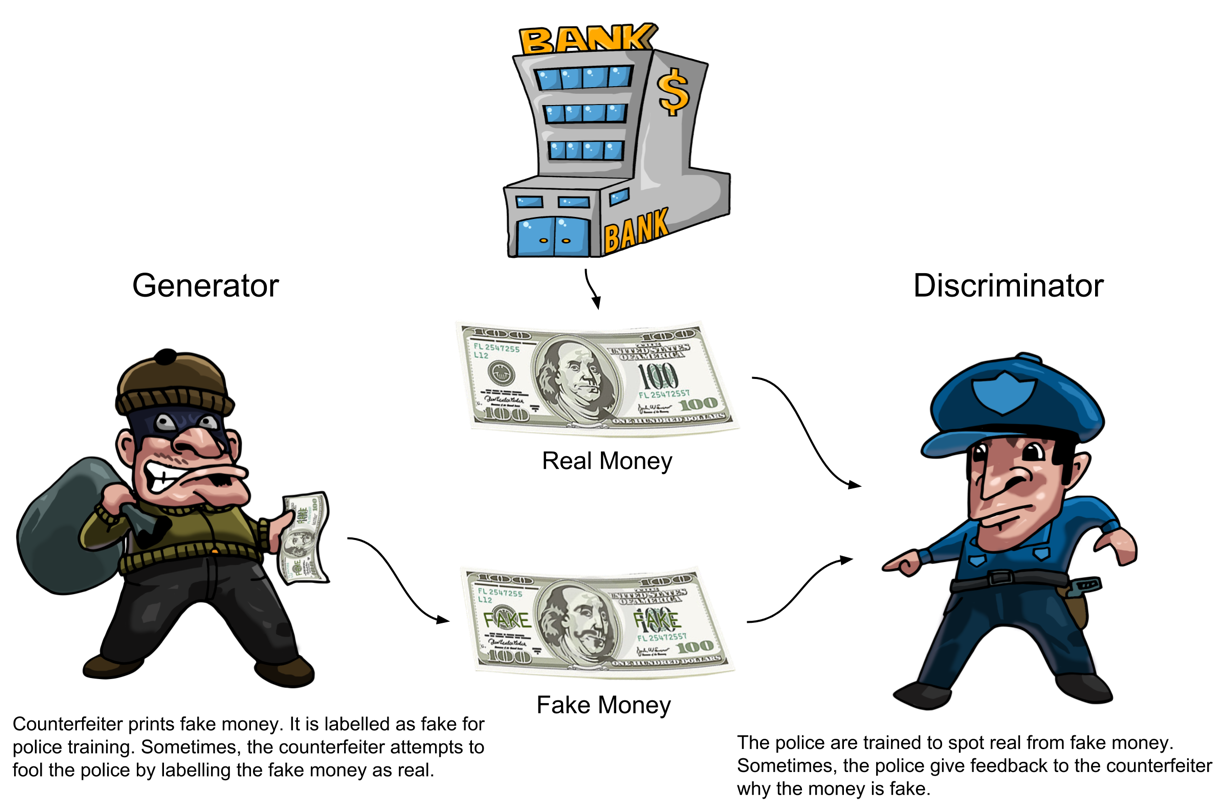
\includegraphics[width=15cm]{images/2_7.png}
\caption{Minh hoạ bộ sinh và bộ phân biệt trong mạng GAN \cite{richardgan2018}.}
\label{fig:thiefandpolice}
\end{figure}

Mục tiêu cuối cùng của GAN là người làm tiền giả phải có khả năng làm tiền giả sao cho cảnh sát không phân biệt được đâu là thật đâu là giả (50/50) để đem tiền giả đi tiêu thụ.
Trong quá trình huấn luyện mạng GAN, thì nhiệm vụ của cảnh sát là học cách phân biệt tiền giả và tiền thật, bên cạnh đó là nói cho người làm tiền giả là nên làm giả như thế nào cho giống thật hơn.
Dần dần thì người làm tiền giả sẽ làm ra được tiền giống tiền thật và cảnh sát cũng trở nên thành thạo trong việc phân biệt tiền thật hay giả.

Ý tưởng của GAN bắt nguồn từ \href{https://cs.stanford.edu/people/eroberts/courses/soco/projects/1998-99/game-theory/nonzero.html}{Non-Zero-Sum Games}\footnote{Stanford, \lq Non-Zero-Sum Games\rq, \href{https://stanford.io/3nCiLKq}{https://stanford.io/3nCiLKq}}, là một trò chơi đối kháng giữa 2 người.
Nếu một trong hai người thắng, thì người còn lại sẽ thua.
Ở mỗi lượt, thì cả 2 đều muốn tối đa hoá cơ hội thắng của mình và tối thiểu hoá cơ hội thắng của đối phương.
Trong lý thuyết trò chơi thì mô hình sẽ hội tụ khi cả bộ sinh và bộ phân biệt đạt tới trạng thái cân bằng Nash\footnote{Jørgen Veisdal, \lq The Nash equilibrium, explained\rq, \href{https://bit.ly/3ea57Lr}{https://bit.ly/3ea57Lr}}, tức là các bước tiếp theo của bất cứ ai trong hai người đều không làm thay đổi cơ hội thẳng của ai cả.

\subsection{Cở sở toán học và hàm mục tiêu (mất mát) của mạng GAN}

Dưới góc độ toán học, một bộ sinh sẽ sinh ra dữ liệu tốt (dữ liệu mà chúng ta mong muốn) nếu ta không thể chỉ ra đâu là dữ liệu giả và đâu là dữ liệu thật.
Trong thống kê, điều này được gọi là bài kiểm tra từ hai tập mẫu - một bài kiểm tra để trả lời câu hỏi liệu tập dữ liệu $\bm{X} = \{x_1, x_2, \dots, x_n\}$ và $\bm{X'}=\{x_1', x_2', \dots, x_n'\}$ có được rút ra từ cùng một phân phối hay không.
Sự khác biệt chính giữa hầu hết những bài nghiên cứu thống kê và GAN, là GAN sử dụng ý tưởng này theo kiểu có tính xây dựng.
Nói cách khác, thay vì chỉ huấn luyện mô hình để nói ``này, hai tập dữ liệu đó có vẻ như không đến từ cùng một phân phối'', thì GAN sử dụng phương pháp \textbf{kiểm tra trên hai tập mẫu}\footnote{Wikipedia, \lq Two-sample hypothesis testing\rq, \href{https://bit.ly/3vmFwVD}{https://bit.ly/3vmFwVD}} để cung cấp tín hiệu cho việc huấn luyện cho bộ sinh.
Điều này cho phép ta cải thiện bộ sinh để có thể sinh dữ liệu tới khi ra được thứ gì đó giống như dữ liệu thực.
Ở mức tối thiểu nhất, nó cần phải lừa được bộ phân biệt, kể cả bộ phân biệt của ta là một mạng nơ-ron sâu tân tiên nhất.

\begin{figure}[!h]
\captionsetup{width=0.8\textwidth}
\centering
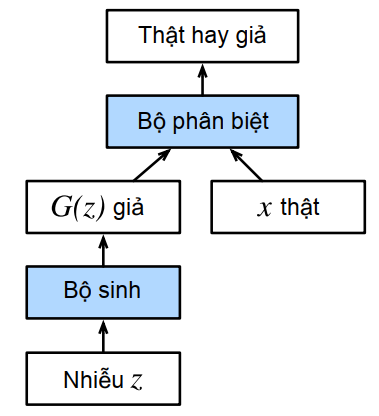
\includegraphics[width=7cm]{images/2_71.PNG}
\caption{Kiến trúc mạng đối nghịch tạo sinh.}
\label{fig:architectsimplegan}
\end{figure}

Bộ phân biệt $D\left(\cdot\right)$ là một mạng học sâu phân loại nhị phân nhằm phân biệt đầu vào $\mathbf{x} \in \mathbb{R}^n$ là thật (từ dữ liệu thật) hoặc giả (từ bộ sinh) (hình \ref{fig:architectsimplegan}), được học theo kiểu giám sát.
Đầu ra của bộ phân biệt là một số vô hướng $o \in \mathbb{R}$ dự đoán cho đầu vào $\mathbf{x}$, và sẽ được đưa qua hàm sigmoid $S(x) = 1/(1 + e^{-x}), \bm{R} = (0, 1)$ để nhận được xác suất dự đoán với giá trị càng gần 1 thì bộ phân biệt càng có xu hướng quyết định đó là dữ liệu thật.
Giả sử mỗi cặp dữ liệu huấn luyện thứ $i$ có dạng $\left(\mathbf{x}_i, y_i\right) \in \mathbb{R}^n\times\{0, 1\}$.
Bộ phân biệt cần được tối ưu sẽ có dạng entropy chéo \cite{wikicrossentropy2021}, nghĩa là:
\begin{align}
    D^*=\arg\min_{D}\left\{-\dfrac{1}{N}\sum_{i=1}^{N}\left[y_i\log D\left(\mathbf{x}_i\right) + \left(1-y_i\right)\log\left(1-D\left(\mathbf{x}_i\right)\right)\right]\right\}\label{eqn:crossentropy}
\end{align}

Còn đối với bộ sinh $G\left(\cdot\right)$ - cũng là một mạng học sâu, sẽ được học theo kiểu không giám sát.
Trước tiên nó cần được cho vài tham số ngẫu nhiên được xem là nhiễu $\mathbf{z} \in \mathbb{R}^d$ từ một nguồn\footnote{Số chiều $d$ của nhiễu đầu vào cũng có ảnh hưởng tới kết quả của mô hình GAN.
Và không có một con số nào là tuyệt đối tốt nhất cho mọi kiến trúc \cite{padala2020effect}.}, ví dụ phân phối chuẩn $\mathbf{z} \sim \mathcal{N}\left(\mu, \sigma^2\right)=\mathcal{N}\left(0, 1\right)$.
Ta thường gọi $\mathbf{z}$ như là một biến tiềm ẩn.
Mục tiêu của mạng sinh là đánh đánh lựa bộ phân biệt để phân loại $\mathbf{x'} = G\left(\mathbf{z}\right)$ là dữ liệu thật, nghĩa là, ta muốn $D\left(G\left(\mathbf{z}\right)\right) \approx 1$.
Một cách diễn đạt khác, cho trước một bộ phân biệt $D$, ta sẽ cập nhật tham số của bộ sinh $G$ nhằm cực đại hoá mất mát entropy chéo như trong (\ref{eqn:crossentropy}) khi $y=0$, tức là:
\begin{align}
    G^*&=\arg\max_G\left\{-\dfrac{1}{N_{\text{nhiễu}}}\sum_{i=1}^{N_{\text{nhiễu}}}\left(1-y_i\right)\log\left(1-D\left(G\left(\mathbf{z}_i\right)\right)\right)\right\}\nonumber\\
    &=\arg\max_G\left\{-\dfrac{1}{N_{\text{nhiễu}}}\sum_{i=1}^{N_{\text{nhiễu}}}\log\left(1-D\left(G\left(\mathbf{z}_i\right)\right)\right)\right\}\label{eqn:dloss}
\end{align}

Trong thực tế, công thức (\ref{eqn:dloss}) không phải là một công thức tốt để tối ưu $G$ \cite{optimizegan2017}.
Là bởi vì, khi mới bắt đầu huấn luyện, bộ sinh $G$ gần như không có khả năng sinh được dữ liệu có phân phối gần giống với phân phối ta cần.
Khả năng cao là ta sẽ có $D\left(G\left(\mathbf{z}\right)\right) \approx 0 \Leftrightarrow \left(1-D\left(G\left(\mathbf{z}\right)\right)\right) \approx 1$.
Mà ta dễ dàng thấy, độ dốc hay chính là đạo hàm của hàm $\log(x)$ giảm khi $x:0\rightarrow 1$ (hình \ref{fig:logbx}, xét cơ số $b = e$).

\begin{figure}[!h]
\captionsetup{width=0.8\textwidth}
\centering
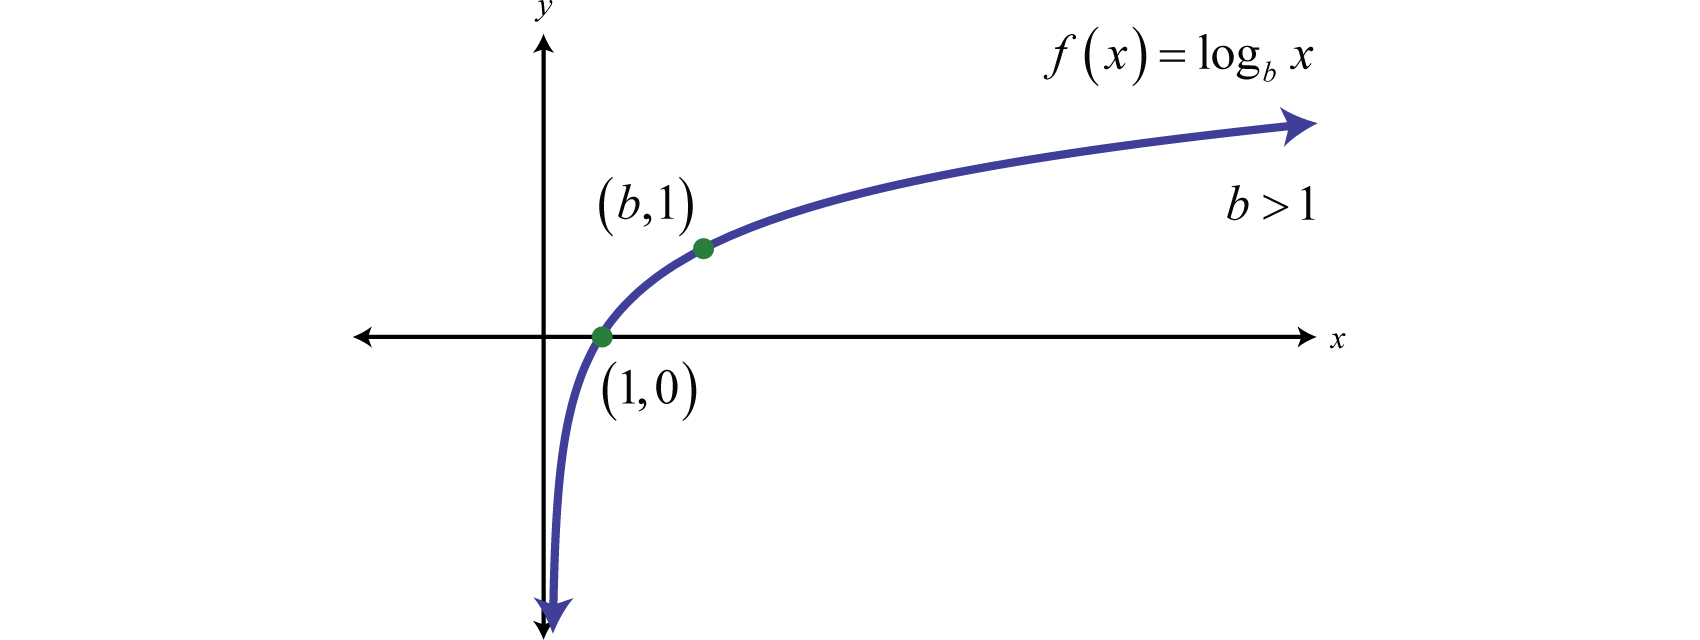
\includegraphics[width=14cm]{images/logx.png}
\caption{Đồ thị hàm $\log_bx$.}
\label{fig:logbx}
\end{figure}

Nếu như $x$ gần giá trị $1$, đạo hàm của $\log(x)$ sẽ bé.
Dễ gây hiện tượng biến mất gradient \cite{wikivanishing2021}, không cập nhật tham số được cho $G$.
Thay vào đó, khi tối ưu $G$, ta sẽ sử dụng chiến lược cực tiểu hoá mất mát entropy chéo như trong (\ref{eqn:crossentropy}) với $y=1$:
\begin{align}
    G^*&=\arg\min_G\left\{-\dfrac{1}{N_{\text{nhiễu}}}\sum_{i=1}^{N_{\text{nhiễu}}}y_i\log\left(D\left(G\left(\mathbf{z}_i\right)\right)\right)\right\}\nonumber\\
    &=\arg\min_G\left\{-\dfrac{1}{N_{\text{nhiễu}}}\sum_{i=1}^{N_{\text{nhiễu}}}\log\left(D\left(G\left(\mathbf{z}_i\right)\right)\right)\right\}\label{eqn:objforrealg}
\end{align}

Khi làm như vậy, ta sẽ có đạo hàm của $\log\left(D\left(G\left(\mathbf{z}\right)\right)\right)$ tại giá trị $D\left(G\left(\mathbf{z}\right)\right) \approx 0$ là lớn hơn so với (\ref{eqn:dloss}), tránh va phải việc gradient biến mất.
Vì đạo hàm của $\log(x)$ khi $x$ ở gần $0$ lớn hơn khi $x$ ở gần $1$.\vspace{5pt}

Tóm lại, $D$ và $G$ đang chơi trò ``cực tiểu hoá cực đại'' với một hàm mục tiêu toàn diện như sau:
\begin{align}
    (D, G)^* &= \arg\min_D\arg\max_G\left\{-\mathbb{E}_{\mathbf{x}\sim \text{dữ liệu thật}}\log D\left(\mathbf{x}\right)-\mathbb{E}_{\mathbf{z} \sim \text{nhiễu}}\log\left(1-D\left(G\left(\mathbf{z}\right)\right)\right)\right\}\label{eqn:minusegan}\\
    \Leftrightarrow (D, G)^* &= \arg\min_G\arg\max_D\left\{\mathbb{E}_{\mathbf{x}\sim \text{dữ liệu thật}}\log D\left(\mathbf{x}\right)+\mathbb{E}_{\mathbf{z} \sim \text{nhiễu}}\log\left(1-D\left(G\left(\mathbf{z}\right)\right)\right)\right\}\label{eqn:egan}
\end{align}

Phép toán $\mathbb{E}\{\cdot\}$ trong [(\ref{eqn:minusegan}), (\ref{eqn:egan})] chính là kì vọng toán, tương đương việc lấy trung bình của tất cả dữ liệu.\vspace{5pt}

Từ hàm mất mát (\ref{eqn:egan}), ta nhận thấy rằng việc huấn luyện bộ phân biệt và bộ sinh là đối nghịch nhau.
Trong khi $D$ cố gắng cực đại mất mát thì $G$ lại đi theo hướng cực tiểu mất mát.
Về mặt lý thuyết, quá trình dạy học cho GAN kết thúc khi mô hình GAN đạt đến trạng thái cân bằng của hai bộ trong mạng, tức cân bằng Nash.

\subsection{Quá trình huấn luyện mạng GAN}

\begin{figure}[!h]
\captionsetup{width=0.8\textwidth}
\centering
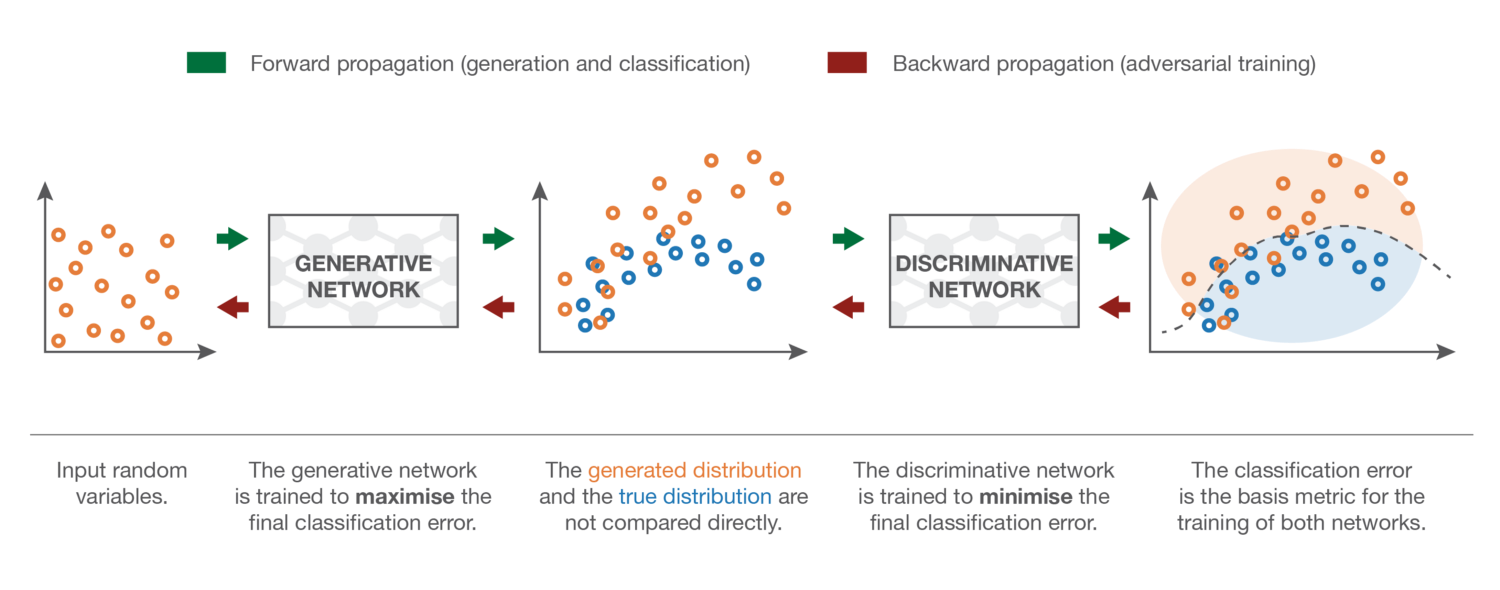
\includegraphics[width=16.5cm]{images/2_72.png}
\caption{Mô phỏng quá trình huấn luyện mạng GAN \cite{josephgan2019, josephroccagan}.}
\label{fig:forandbackgan}
\end{figure}

Huấn luyện mạng GAN cũng không quá phức tạp nhưng lại tinh vi (hình \ref{fig:forandbackgan}) nên cần được giới thiệu.
Sẽ có hai phiên: lan truyền thuận và lan truyền ngược.
Ở phiên lan truyền thuận, ta chọn ngẫu nhiên $b$ vector nhiễu từ một phân phối nhiễu xác định trước $\mathbf{Z} = \left[\mathbf{z}_1, \mathbf{z}_2, \dots, \mathbf{z}_b\right] \in \mathbb{R}^{d \times b}$ rồi tạo ảnh:
\begin{align}
    \mathbf{X'} &= \left[\mathbf{x'}_1, \mathbf{x'}_2, \dots, \mathbf{x'}_b\right]\nonumber\\
                &= G\left(\mathbf{Z}\right)\nonumber\\
                &= \left[G\left(\mathbf{z}_1\right), G\left(\mathbf{z}_2\right), \dots, G\left(\mathbf{z}_b\right)\right] \in \mathbb{R}^{n \times b}
\end{align}

Những ảnh được tạo ra sẽ được gán nhãn $y=0$, kết hợp với $b$ vector\footnote{Việc chọn số lượng mẫu từ tập dữ liệu thật nên là bằng số lượng mẫu từ dữ liệu giả, sẽ tránh được hiện tượng không cân bằng khi huấn luyện một bộ phân loại \cite{jasonimbalance2019}.} chọn từ tập dữ liệu thật $\mathbf{X} = \left[\mathbf{x}_1, \mathbf{x}_2, \dots, \mathbf{x}_b\right] \in \mathbb{R}^{n \times b}$ được gán nhãn $y=1$.
Đầu vào của bộ phân biệt sẽ là $\mathbf{\bar{X}} = \left[\mathbf{X'}, \mathbf{X}\right] \in \mathbb{R}^{2b \times n}$ để phân loại.
Hoành thành phiên lan truyền thuận.
Kết quả phân loại là các xác suất xem mỗi điểm dữ liệu là thuộc dữ liệu thật hay là giả:
\begin{align}
    \widehat{\mathbf{Y}}_D &= D\left(\mathbf{\bar{X}}\right) = D\left(\left[\mathbf{X'}, \mathbf{X}\right]\right)\nonumber\\
                &= \left[D\left(\mathbf{x'}_1\right), D\left(\mathbf{x'}_2\right), \dots, D\left(\mathbf{x'}_b\right), D\left(\mathbf{x}_1\right), D\left(\mathbf{x}_2\right), \dots, D\left(\mathbf{x}_b\right)\right]\nonumber\\
                &= \left[\widehat{y}_{D; 1}, \widehat{y}_{D; 2}, \dots, \widehat{y}_{D; 2b}\right] \in \mathbb{R}^{1 \times 2b}
\end{align}

Sau khi có được $\widehat{\mathbf{Y}}_D$, ta bắt đầu phiên lan truyền ngược bằng việc lấy nhãn $\mathbf{Y}_D=[\underbrace{0, 0, \dots, 0}_{b \text{ mẫu}}, \underbrace{1, 1, \dots, 1}_{b \text{ mẫu}}] \in \mathbb{R}^{1 \times 2b}$ để đưa vào hàm mất mát (\ref{eqn:crossentropy}) và tối ưu bằng gradient thông qua một thuật toán tối ưu \cite{ruder2017overview}.
Sau khi tối ưu, bộ phân biệt sẽ có trở nên tốt hơn trong việc phân biệt hai phân phối.
Một nửa của phiên lan truyền ngược đã được hoàn thành.\vspace{5pt}

Một nửa còn lại của phiên lan truyền ngược tiếp tục.
Ta cần cố định các gradient của $D$, rồi lấy kết quả tính được trong phiên trước $\widehat{\mathbf{Y}}_D = D\left(\mathbf{X'}\right) = \left[\widehat{y}_{D; 1}, \widehat{y}_{D; 2}, \dots, \widehat{y}_{D; b}\right] \in \mathbb{R}^{1 \times b}$, rồi cùng với nhãn $\mathbf{Y}_D=\left[1, 1, \dots, 1\right] \in \mathbb{R}^{1 \times b}$ được truyền vào hàm mất mát (\ref{eqn:objforrealg}), và ta cũng sẽ tối ưu bằng gradient thông qua một thuật toán tối ưu.
Vì trong (\ref{eqn:objforrealg}) cũng có cùng $D$, nên như đã đề cập ban đầu, các gradient của $D$ cần được cố định lại trước khi huấn luyện $G$.
Qua mỗi lượt tố ưu, phân phối của tập ảnh sẽ được điều chỉnh cho giống với phân phối tập dữ liệu thật.\vspace{5pt}

Trong suốt quá trình tối ưu, phân phối nhiễu được giữ nguyên.
Việc thay đổi phân phối này làm phức tạp thêm cho công cuộc huấn luyện mà cũng chưa chắc đem lại kết quả khả quan hơn.

\subsection{Sự thông minh trong ý tưởng của mạng GAN}

Thực sự mà nói, nếu ta có thể biết được cách biểu diễn cụ thể cho phân phối dữ liệu thật, thì việc sinh đã trở nên đơn giản.
Tuy nhiên, vì việc đó là bất khả thi, nên những thuật toán mới được sinh ra.
Nhằm để tìm ra một ánh xạ, sao cho từ một tập đích là một phân phối đơn giản, ta có được kết quả ánh xạ nằm trên một phân phối tương tự với phân phối dữ liệu thật - thứ mà ta không biết cụ thể.\vspace{5pt}

Đã từng có một cách tiếp cận GMN (\textbf{G}enerative \textbf{M}atching \textbf{N}etworks)\footnote{GMN không phải là một mô hình cụ thể mà là một loại phương pháp.}.
Phương pháp này sẽ so sánh phân phối của ảnh ánh xạ với phân phối dữ liệu thật dự vào các mẫu từ hai tập.
Dẫu vậy, việc cài đặt và huấn luyện cần một phép đo hợp lý để so sánh hai phân phối là một điều không hề dễ dàng \cite{replyganovergmn2019}.
Và hay thay, GAN đưa ra một giải pháp thông minh, là mượn một mạng học sâu khác để giải quyết.
Nhờ vào việc để bộ phân biệt - một mạng học sâu không quá phức tạp để tối ưu dẫn đường, công việc của ta bây giờ sẽ chỉ là tập trung nhiều cho tối ưu ánh xạ bộ sinh.\vspace{5pt}

Nếu đi đủ sâu, ta sẽ nhận thấy rằng, việc GAN làm thực sự không phải là giúp cho phân phối tập ảnh giống hoàn toàn với phân phối thật.
Mà phức tạp hơn, GAN đang cực tiểu hoá khoảng cách giữa hai phân phối.
Điều này giúp GAN sinh ra được những thứ không chỉ giống mà còn là những điều tiềm ẩn ở trong dữ liệu có sẵn \cite{gregoiregan2019}.

\subsection{Mạng GAN không hoàn hảo}

Một điều tệ khó tránh khỏi giống như nhiều mạng học sâu khác, GAN đôi khi cũng sẽ không hội tụ \cite{barnett2018convergence}.
Xét một ví dụ trong không gian 2D (hình \ref{fig:divgan}), mạng GAN chỉ có thể sinh ra phân phối liên thông tại xung qua 1 vị trí nào đó.
Tuy nhiên, phân phối ta mong muốn lại không liên thông mà rải rác ở nhiều vùng, bộ phân biệt cũng vì thế sẽ cho điểm thấp (tức đánh giá không thật) do bộ sinh chưa đáp ứng đạt yêu cầu.
Dựa vào đó, bộ sinh chuyển phân phối của mình sang chỗ khác.
Và đương nhiên khi chuyển, là chuyển toàn bộ phân phối đi chứ không giữ lại một phần ở phân phối cũ.
Nhưng trắc trở thay, tại một thời điểm, phân phối tập ảnh chỉ có thể ở một nơi trong rất nhiều nơi trong phân phối dữ liệu thật.
Nên kết quả luôn luôn bị bộ phân biệt cho điểm thấp.
Dẫn đến bộ sinh mãi mãi không bao giờ thấy mình có tiến bộ và phân kỳ.

\begin{figure}[!h]
\captionsetup{width=0.8\textwidth}
\centering
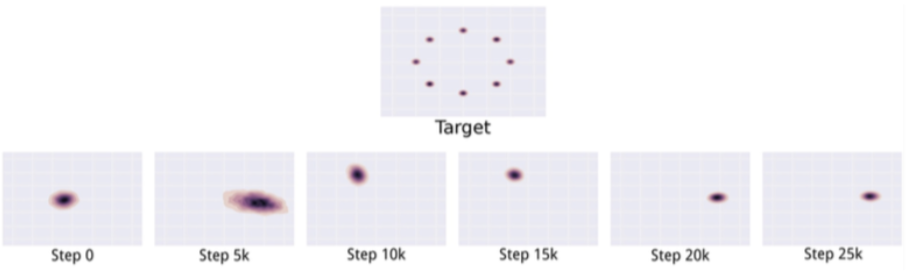
\includegraphics[width=15cm]{images/divgan.PNG}
\caption{GAN không có khả năng sinh ra được phân phối (hàng dưới) gần giống với phân phối được chọn (hàng trên) \cite{metz2017unrolled}.}
\label{fig:divgan}
\end{figure}

\section{Mạng tích chập Unet}\label{unetarchitecture}

\subsection{Khái quát về tích chập và mạng tích chập}\label{convolutionnet}

\begin{wrapfigure}{l}{0pt}
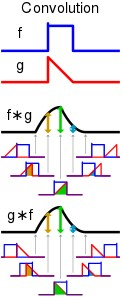
\includegraphics[width=3.4cm]{images/convolution.jpg} 
\caption{Minh hoạ tích chập giữa hai hàm số $f$ và $g$.}
\label{fig:convof2functions}
\end{wrapfigure}

Sự đột phát trong ngành thị giác máy tính, hẳn khó tìm được ai trong những người đã có kinh nghiệm trong lĩnh vực này, phủ nhận việc công lớn thuộc về mạng tích chập - một loại mạng học sâu.
Nó giúp giải quyết những bài toán phân loại hình ảnh, xem một tấm ảnh bất kì là ảnh về một con chó hay là của một con mèo, hoặc là một thứ gì khác \cite{wikialexnet2021}.
Công nghệ nhận diện khuôn mặt được chính xác hơn cũng là nhờ ứng dụng mạng tích chập \cite{faceregusingcnn2019}.
Nếu chỉ dừng lại ở mỗi khuôn mặt, thì cũng đã là rất thành công.
Nhưng ý tưởng tích chập này còn có thể áp dụng được cho mọi loại đối tượng khác trong bài toán nhận diện \cite{objregusingcnn2019} cũng như nhiều bài toán khác về xử lý ảnh \cite{applofcnnpune2016}.\vspace{5pt}

Tích chập \cite{wikiconv2021}, là một phép toán giữa hai hàm số $f, g$ dùng để tạo ra một hàm số khác $f \ast g$, hàm số này miêu tả hình thù của đồ thị hàm $f$ bị thay đổi bởi hàm $g$ (hình \ref{fig:convof2functions}).
Ta cũng có thể nói ngược lại là $g$ bị thay đổi bởi $f$ vì tích chập có tính chất giao hoán.
Ý nghĩa của việc này, $f \ast g$ cho ta biết độ giống nhau giữa hai hàm $f$ và $g$ ở mỗi điểm.\vspace{5pt}

Ứng dụng điều này, các nhà khoa học đã thử lấy ảnh - là một ma trận số [\textbf{\ref{intro2ditimg}}] $\mathcal{I} \in \bm{G}^{W \times H}$ làm $f$.
Và sử dụng những ảnh bé hơn $\mathcal{K} \in \mathbb{R}^{\dim\left(\bm{G}\right) \times K \times K}$ miêu tả những cạnh, màu để làm $g$.
Những ảnh này thường được gọi là các bộ lọc và mỗi lần tích chập chỉ dùng một bộ lọc.
Để tính tích chập \cite{wikikernalimgpro2021}, họ trượt bộ lọc này đi khắp ảnh theo một bước nhảy $S$ cố định, kèm thêm đệm $P$ \cite{dl2sandp2021} cho ảnh để phù hợp kích thước nếu cần thiết.
Ở từng vị trí được trượt, ta lần lượt trích xuất vùng ảnh tương ứng mà bộ lọc được đặt lên $\mathcal{I}_{m:m + K - 1, n: n + K - 1} \in \bm{G}^{K \times K}$, sau đó sử dụng công thức:
\begin{align}
    \left(\mathcal{I} \ast \mathcal{K}\right)_{m*, n*}=\sum_{k=1}^{\dim\left(\bm{G}\right)}\sum_{i=0}^K\sum_{j=0}^K\mathcal{I}^{\left(k\right)}_{m+i,n+j}\mathcal{K}^{\left(k\right)}_{i+1, j+1}\label{eqn:convformula}
\end{align}

Trong đó, toạ độ $(m*, n*)$ là vị trí kết quả của việc áp ảnh bộ lọc lên phần $\mathcal{I}_{m:m + K - 1, n: n + K - 1}$ (hình \ref{fig:convoperator}).
Toạ độ này sẽ thay đổi tuỳ thuộc vào bước nhảy, đệm, cũng như là kích thước bộ lọc mà ta sử dụng.
Kết quả sẽ là một số vô hướng, biểu thị sự giống nhau giữa bộ lọc và vùng ảnh được chọn.\vspace{5pt}

Để triển khai công thức (\ref{eqn:convformula}) trên máy tính, ta sẽ phải áp dụng những vòng lặp.
Nhưng điều đó sẽ làm chậm tốc độ tính toán đi rất nhiều.
Thay vào đó, một giải pháp được đưa ra đó là trải dài 2 ảnh ra thành một vector và tính tích vô hướng \cite{wikidotproduct2021}.
Việc trải ảnh ra để tính tích vô hướng là để tận dụng phép toán ma trận, tối ưu các luồng nhân để tăng tốc độ tính toán \cite{matrixcalfaster2018}.\vspace{5pt}

\begin{figure}[!h]
\captionsetup{width=0.8\textwidth}
\centering
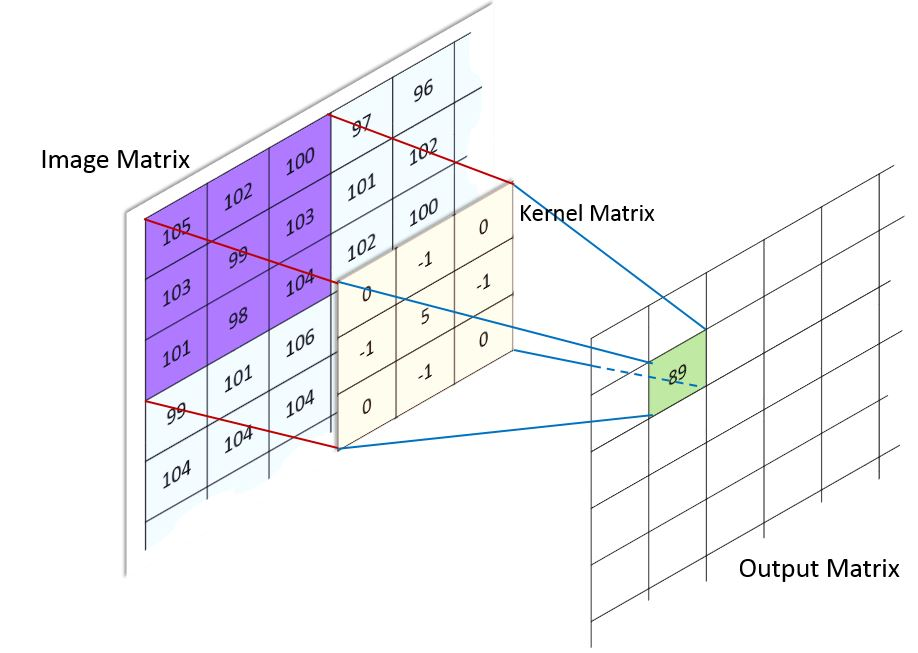
\includegraphics[width=15cm]{images/convinimage.jpg}
\caption{Minh hoạ tính tích chập với bộ lọc kích thước $3 \times 3$.}
\label{fig:convoperator}
\end{figure}

Kích thước cuối cùng của ảnh đầu ra (giả sử ảnh đầu vào là một ảnh vuông, tức chiều rộng bằng chiều cao $W = H$) sau khi trượt một bộ lọc kích thước $K \times K$, bước nhảy $S$ và đệm $P$ từ ảnh gốc là \cite{replycalcnnsize}:
\begin{align}
    W_{\text{đầu ra}} = \left\lfloor\dfrac{W_{\text{đầu vào}} - K + 2P}{S}\right\rfloor + 1\label{eqn:cnnsize}
\end{align}

Công thức (\ref{eqn:cnnsize}) sẽ là cần thiết khi ta quan tấm đến vùng nhận thức, để hiểu rõ về kiến trúc PatchGAN [\textbf{\ref{patchdiscriminator}}].\vspace{5pt}

Mạng tích chập là mạng kết hợp nhiều bộ lọc theo một kiến trúc nào đó, nhằm trích lọc được các đặc trưng từ ảnh (như mắt, mũi, miệng từ ảnh mặt người).
Điều này giúp cho bài toán được giải quyết một cách đơn giản, hiệu quả hơn cho các tác vụ về ảnh, khi ta chỉ cần tập trung vào thứ cần tập trung nhờ bộ lọc.
Thay vì những mạng học sâu thông thường, ta sẽ đưa tất cả những thông tin của ảnh đầu vào (ở mức đơn giản nhất, là toàn bộ điểm ảnh).\vspace{5pt}

Khái niệm bộ lọc đã có trước khi có mạng học sâu tích chập, những bộ lọc này được con người tính toán thông qua những nghiên cứu.
Rồi từ đó cũng trích xuất các đặc trưng và đưa vào các thuật toán học máy.
Nhưng với học sâu, quá trình tìm ra bộ lọc được tích hợp vào trong quá trình huấn luyện mạng (hình \ref{fig:mlvsdlindip}).
Giúp tìm ra những bộ lọc thích hợp nhất với mỗi tập dữ liệu bất kỳ.\vspace{5pt}

Chỉ với phép tính tích vô hướng đơn giản như vậy, nhưng lại ảnh hưởng sâu sắc đến không chỉ trong mảng thị giác, mà còn được ứng dụng sang nhiều mảng khác.
Khi người ta nhận thấy sức mạnh của tích chập, rất nhiều kiểu dữ liệu đã được cố gắng đẩy về dạng hình ảnh để ứng dụng mạng tích chập, chẳng hạn như âm thanh \cite{soundusingcnnieee, papiasoundcnn2021}.

\begin{figure}[!h]
\captionsetup{width=0.8\textwidth}
\centering
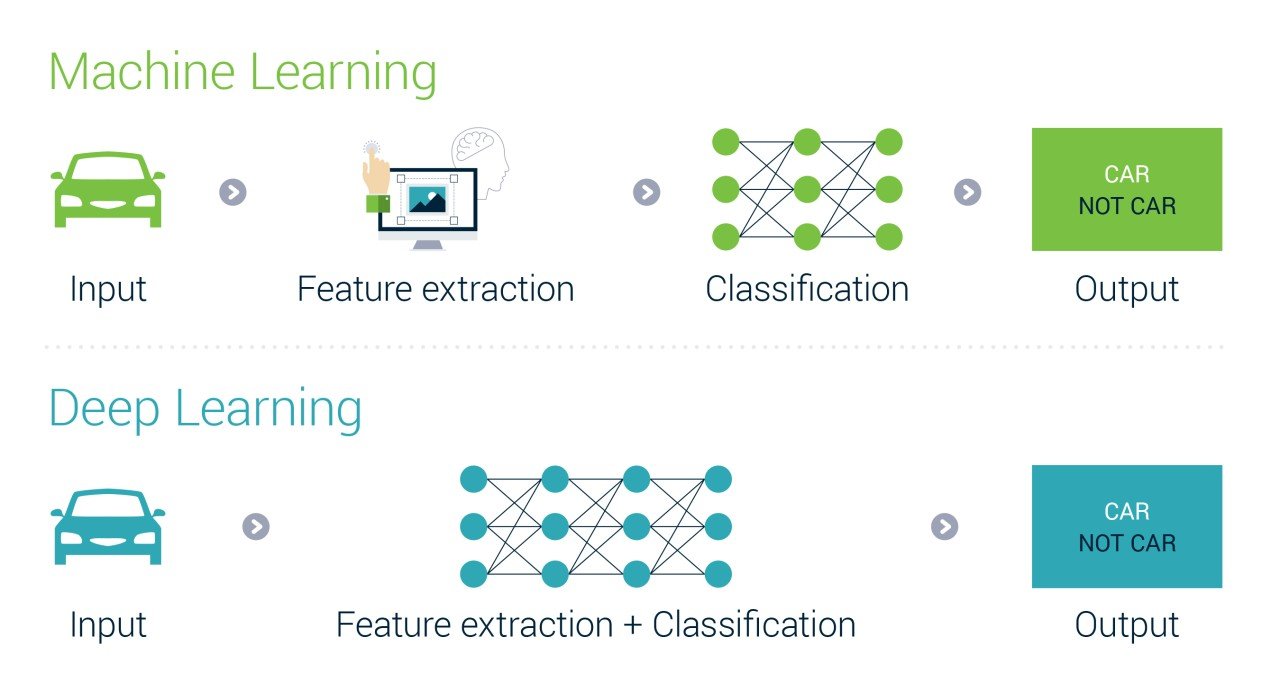
\includegraphics[width=15cm]{images/mlvsdlindip.jpg}
\caption{Sự khác biệt giữa hai quá trình học máy và học sâu trong việc xử lý ảnh.}
\label{fig:mlvsdlindip}
\end{figure}

Trích lọc đặc trưng không phải là mục tiêu duy nhất khiến mọi người sử dụng tích chập.
Mà còn là vì nó có thể hỗ trợ trong việc giảm các loại nhiễu cơ bản của ảnh đầu vào \cite{fu2018convolutional} (hình \ref{fig:mylady_denoise}), làm mờ ảnh nếu cần thiết \cite{szandala2020convolutional},..

\begin{figure}[!h]
\captionsetup{width=0.8\textwidth}
\centering
\includegraphics[width=15cm]{images/mylady_denoise.png}
\caption{(a) Ảnh có nhiễu. (b) Ảnh sau khi được giảm nhiễu bằng bộ lọc $3 \times 3$. (b) Ảnh sau khi được giảm nhiễu bằng bộ lọc $7 \times 7$ \cite{mlcobancnn2018}.}
\label{fig:mylady_denoise}
\end{figure}

\subsection{Kiến trúc Unet}

Unet là một kiến trúc tích chập, được phát triển nhằm phân vùng các cấu trúc nơ-ron thần kinh trong não người.
Kiến trúc này lần đầu được áp dụng đã giành chiến thắng trong cuộc thi EM segmentation challenge at ISBI 2012.\footnote{ISBS Challenge: Segmentation of neuonal structures in EM stacks, \href{https://bit.ly/2RAIyqR}{https://bit.ly/2RAIyqR}}\vspace{5pt}

Unet bao gồm 2 nhánh đối xứng nhau hình chữ U nên được gọi là Unet.
Nhánh ở bên trái là thu hẹp, còn phần mở rộng là nhánh ở bên phải.
Mỗi phần sẽ thực hiện một nhiệm vụ riêng như sau:

\begin{itemize}
    \item Phần thu hẹp: làm nhiệm vụ trích lọc đăc trưng để tìm ra bối cảnh của hình ảnh, tức để biết \textbf{CÁI GÌ}.
    Vai trò của phần thu hẹp tương tự như một bộ mã hoá.
    Một mạng tích chập sâu sẽ đảm nhận trích lọc đặc trưng.
    Lý do nhánh được gọi là thu hẹp vì kích thước dài và rộng, chính là độ phân giải, của các tầng giảm dần.
    Độ phân giải được giảm bằng cách sử dụng gộp cực đại \cite{wikimaxpooling2021}, hoặc dùng tích chập có đệm và sải bước hợp lí.
    
    \item Phần mở rộng: Gồm các tầng đối xứng tương ứng với các tầng của nhánh thu hẹp có vai trò như một bộ giải mã.
    Ở phần này, độ phân giải của các tầng được tăng lại để biết được vị trí, tức \textbf{Ở ĐÂU}.
    Từ đó đánh dấu nhãn của từng điểm ảnh.
    Để làm được điều này, ta cần sử dụng kĩ thuật giải chập.
    Có nhiều phương pháp để giải chập, chẳng hạn như sao chép các giá trị điểm ảnh liền kề theo các kích thước cửa sổ \cite{khanhunet2020}.
    Hoặc một phương thức khác là sử dụng tích chập giãn nở \cite{yu2016multiscale}.
    Nhưng được áp dụng nhiều nhất là tích chập chuyển vị \cite{divyanshutransconv2020} cùng với đêm và sải bước thích hợp.
\end{itemize}

\begin{figure}[!h]
\captionsetup{width=0.8\textwidth}
\centering
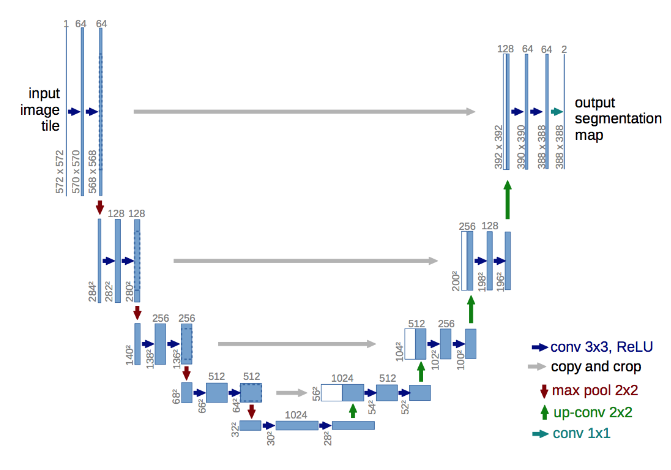
\includegraphics[width=15cm]{images/2_8.png}
\caption{Kiến trúc mô hình mạng Unet \cite{ronneberger2015unet}.}
\end{figure}

Đặc trưng riêng trong cấu trúc của Unet đó là có những kết nối tắt đối xứng giữa các tầng của nhánh bên trái tương ứng với các tầng bên nhánh bên phải.
Việc kết nối tắt theo kiến trúc Unet là một điểm mới so với kiến trúc mã hoá và giải mã thông thường nhằm bổ sung thêm thông tin và gia tăng độ chính xác.
Một số mạng tích chập hiện đại sử dụng như phương pháp trên \cite{he2015deep, huang2018densely} để có thể giúp cho mô hình được sâu hơn, chính xác hơn.\vspace{5pt}

Ngoài ra kết nối tắt còn khắc phục hiện tượng gradient biến mất \cite{adaloglou2020skip}.
Một số nghiên cứu còn có thể chứng minh lý thuyết rằng, những mạng học sâu sử dụng kết nối tắt, ngoài hố cực tiểu toàn cục, các hố cực tiểu còn lại thường rất nông \cite{wang2020skip}.

\begin{figure}[!h]
\captionsetup{width=0.8\textwidth}
\centering
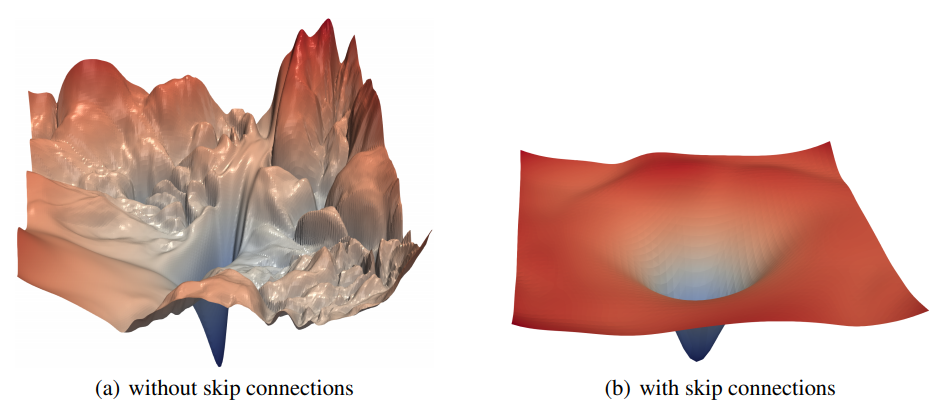
\includegraphics[width=15cm]{images/objwithskip.png}
\caption{Sự khác biệt của bề mặt hàm mục tiêu khi không (a) và có (b) sử dụng kết nối tắt \cite{li2018visualizing}.}
\end{figure}

\section{Kiến trúc pix2pix}\label{pix2pixarchitecture}

Bản thân kiến trúc GAN trong pix2pix cũng không khác mạng GAN [\textbf{\ref{ganarchitecture}}] là bao.
Gồm 2 mạng chính: bộ phân biệt và bộ sinh (hình \ref{fig:pix2pixarchitecture}).
Tuy nhiên, có nhiều điều khác biệt giữa pix2pix so với GAN thông thường.

\begin{figure}[!h]
\captionsetup{width=0.8\textwidth}
\centering
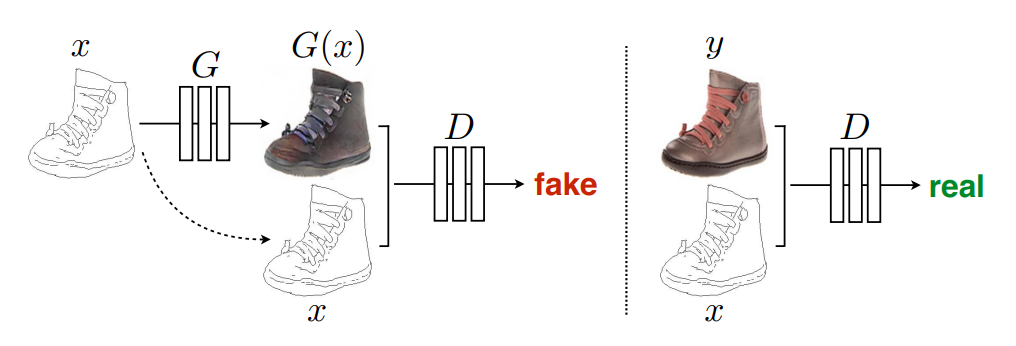
\includegraphics[width=17cm]{images/2_9.PNG}
\caption{Mô hình pix2pix thêm màu sắc cho các nét vẽ để tạo ảnh màu. Một bài toán tương tự với bài toán tạo màu cho ảnh \cite{isola2018imagetoimage}.}
\label{fig:pix2pixarchitecture}
\end{figure}

\subsection{Khái quát mạng GAN trong pix2pix}\label{overviewofpix2pix}

Về bộ sinh, đầu vào bây giờ không còn là một vector nhiễu từ một phân phối chọn trước.
Mà là một bức ảnh nguồn $x$.
Sau đó bức ảnh được truyền vào một kiến trúc mạng tích chập để trích lọc đặc trưng và dùng đặc trưng này biến đổi lại thành ảnh đích $G(x)$.
Các tác giả đã thử nghiệm 2 kiến trúc tích chập để xử lý việc này là Unet [\textbf{\ref{unetarchitecture}}] và mã hoá-giải mã - một kiến trúc giống Unet nhưng không sử dụng kết nối tắt (hình \ref{fig:enc-decvsunet}).
Giữa hai kiến trúc, Unet có kết quả khả quan hơn.\vspace{5pt}

\begin{figure}[!h]
\captionsetup{width=0.8\textwidth}
\centering
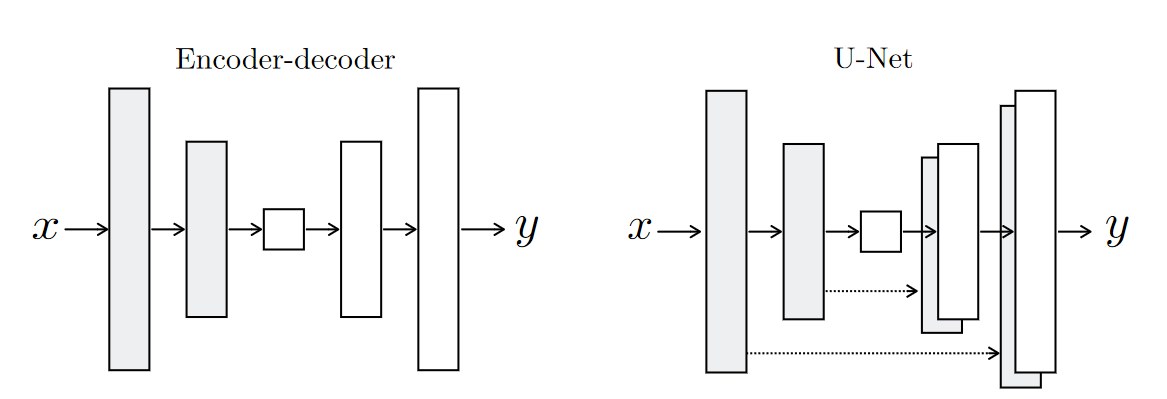
\includegraphics[width=15cm]{images/3_2.PNG}
\caption{Tổng quát kiến trúc mạng mã hoá-giải mã và mạng Unet \cite{isola2018imagetoimage}.}
\label{fig:enc-decvsunet}
\end{figure}

Bộ phân biệt giờ đây sẽ nhận vào một cặp ảnh.
Trong đó luôn có ảnh $x$, được coi là điều kiện cho bộ phân biệt.
Còn ảnh còn lại là ảnh đầu ra.
Ảnh đầu ra có thể là ảnh được tạo ra từ bộ sinh $G(x)$, hoặc là nhãn của ảnh đầu vào được lấy từ tập dữ liệu huấn luyện $y$.
Các cặp ảnh sẽ được gán nhán là thật nếu là $(x, y)$.
Ngược lại sẽ là giả nếu đi kèm là $\left(x, G(x)\right)$.

\subsection{Bộ phân biệt Patch trong pix2pix}\label{patchdiscriminator}

Một điểm khác biệt nữa của bộ phân biệt trong mô hình pix2pix so với những bộ phân biệt trong các mô hình GAN thông thường, là bộ phân biệt của chúng ta là làm việc theo Patch.
Một bộ phân biệt thông thường chỉ trả về một số vô hướng thì bộ phân biệt Patch sẽ trả về một ma trận $\mathbf{P_D} \in \mathbb{R}^{k\times k}$ (hình \ref{fig:patchganarchitecture}).
Mỗi phần tử của ma trận $\left[\mathbf{P_D}\right]_{ij}$ là kết quả phân loại một vùng $N \times N$ của đầu vào là thật hay giả.
Những vùng $N \times N$ này được gọi là vùng nhận thức (hình \ref{fig:receptivefield}).\vspace{5pt}

\begin{figure}[!h]
\captionsetup{width=0.8\textwidth}
\centering
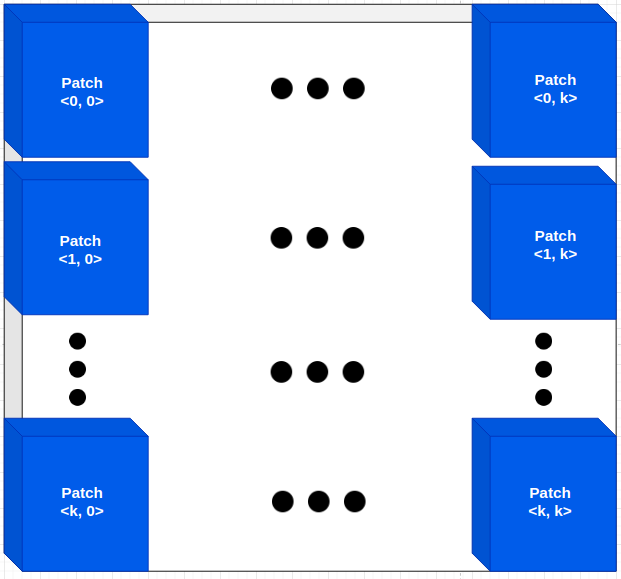
\includegraphics[width=10cm]{images/patch.png}
\caption{Hình ảnh giả sử được đầu vào chia thành $k\times k$ Patch \cite{khanhpix2pix2020}.}
\label{fig:patchganarchitecture}
\end{figure}

Về bản chất, bộ phân biệt Patch vẫn là một kiến trúc mạng tích chập gồm nhiều tầng tích chập liên tiếp nhau.
Nhưng chúng ta không thực hiện làm phẳng ở gần cuối để truyền qua các lớp kết nối đầy đủ rồi cho ra duy nhất một vô hướng.
Mà thay vào đó, tính toán để ra được dự báo xác suất trên mỗi Patch rơi vào ảnh thật.
Xác suất để toàn bộ đầu vào là thật sẽ là trung bình cộng của toàn bộ $k^2$ Patch.
Cách tính như vậy sẽ mang lại hiệu quả nếu áp dụng trên các Patch có kích thước lớn vì có vùng nhận thức lớn hơn.
Kết quả xác suất trung bình của nhiều Patch cũng sẽ chuẩn xác hơn.\vspace{5pt}

Sau khi đã thử qua một số kích thước Patch như $1\times 1, 16\times 16, 70\times 70, 286\times 286$ thì kích thước Patch tốt nhất theo \cite{isola2018imagetoimage} là $70 \times 70$.
Kiến trúc các tầng của một bộ phân biệt Patch $70\times 70$ có thể biểu diễn đơn giản như sau:
\begin{align}
    \text{I} \rightarrow \text{2C64} \rightarrow \text{2C128} \rightarrow \text{2C256} \rightarrow \text{1C512} \rightarrow \text{O}\label{eqn:disarchitecture}
\end{align}

Với $\text{sCk}$ là một tầng tích chập gồm $k$ bộ lọc và có sải bước là $s$.
Tầng cuối cùng $\text{O}$ sử dụng sải bước là $1$ và chỉ sử dụng duy nhất $1$ bộ lọc để trả ra ma trận $\mathbf{P_D}$, rồi kích hoạt hàm sigmoid để lấy xác suất.
Tất cả các tầng đều sử dụng kích thước bộ lọc là $4 \times 4$ cùng với kích thước đệm là $1$.

\begin{figure}[!h]
\captionsetup{width=0.8\textwidth}
\centering
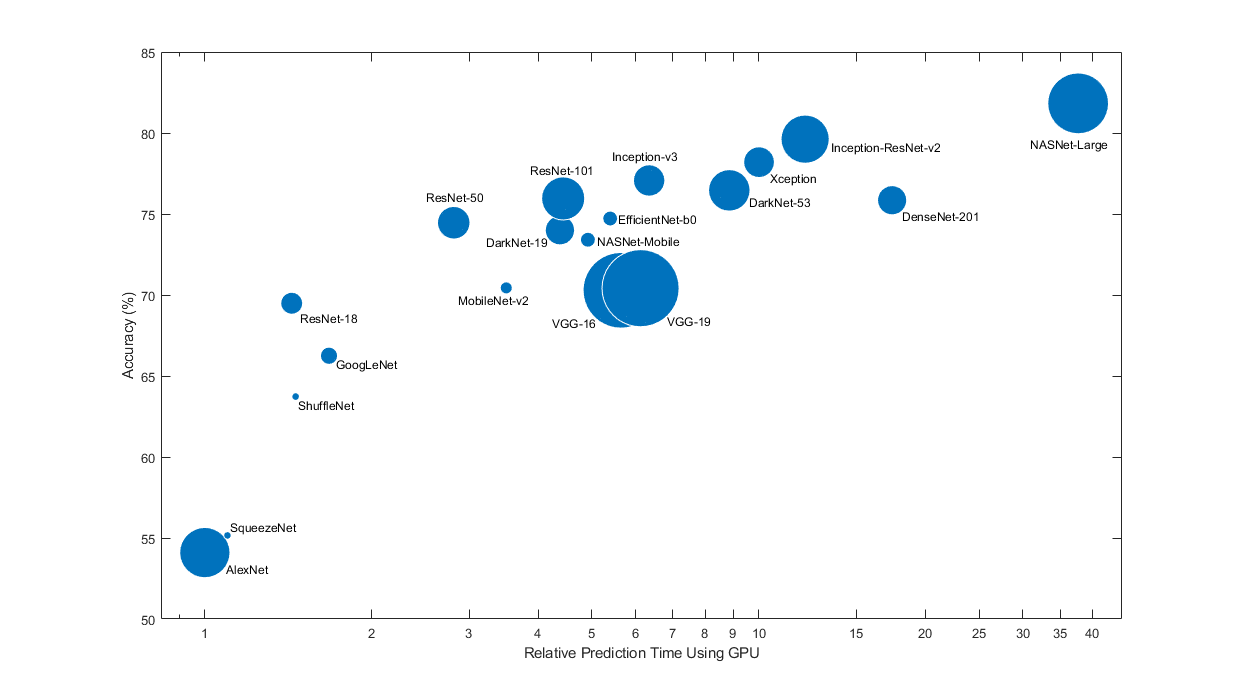
\includegraphics[width=10cm]{images/3_3.png}
\caption{Mô tả vùng nhận thức qua các tầng.}
\label{fig:receptivefield}
\end{figure}

Ta hoàn toàn có thể tính ngược lại được vùng nhận thức dựa vào thông tin kích thước bộ lọc và sải bước.
Từ (\ref{eqn:cnnsize}), bằng các phép biến đổi đại số cơ bản, ta suy ra được:
\begin{align}
    W_{\text{đầu vào}} = K - 2P + S\left(W_{\text{đầu ra}} - 1\right)\label{eqn:inversecnnsize}
\end{align}

Tuy nhiên, khi suy ngược lại để tính vùng nhận thức, vùng nhận thức ta cần quan tâm vùng ảnh không có đệm.
Do đó, điều chỉnh công thức (\ref{eqn:inversecnnsize}), kích thước vùng nhận thức $F$ từng tầng sẽ là:
\begin{align}
    F_{\text{L}} = K + S\left(F_{\text{L+1}} - 1\right)\label{eqn:receptivefieldsize}
\end{align}

Áp dụng công thức (\ref{eqn:receptivefieldsize}), ta sẽ tính được kích thước vùng nhận thức của mỗi giá trị đầu ra của bộ phân biệt Patch $70 \times 70$ (\ref{eqn:disarchitecture}) theo như kết quả sau đây:
\begin{align*}
    F_4 &= K + S_4(F_5 - 1) = 4 + 1(1-1) = 4\\
    F_3 &= K + S_3(F_4 - 1) = 4 + 1(4-1) = 7\\
    F_2 &= K + S_2(F_3 - 1) = 4 + 2(7-1) = 16\\
    F_1 &= K + S_1(F_2 - 1) = 4 + 2(16-1) = 34\\
    F_0 &= K + S_0(F_1 - 1) = 4 + 2(34 - 1) = 70
\end{align*}

Ta có thể mô tả tổng quát kiến trúc các lớp mạng tích chập áp dụng trên một Patch $70 \times 70$ (hình \ref{fig:dis70pix2pix}):

\begin{figure}[!h]
\captionsetup{width=0.8\textwidth}
\centering
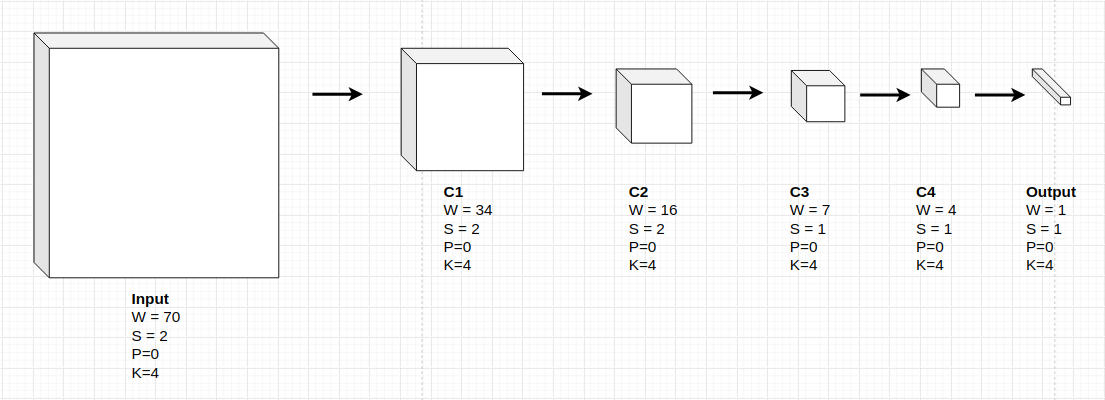
\includegraphics[width=16cm]{images/dis70pix2pix.png}
\caption{Sơ đồ tổng quát kiến trúc các lớp mạng tích chập áp dụng trên một Patch $70 \times 70$.}
\label{fig:dis70pix2pix}
\end{figure}

\subsection{Hàm mục tiêu (mất mát) pix2pix}\label{objofpix2pix}

Hàm mục tiêu của mạng GAN có điều kiện pix2pix gần giống với (\ref{eqn:egan}), được biểu diễn như sau:
\begin{align}
    \mathcal{L}_{cGAN}\left(G, D\right) = \mathbb{E}_{x, y}\left[\log D\left(x, y\right)\right] + \mathbb{E}_{x, z}\left[\log\left(1-D\left(x, G\left(x, z\right)\right)\right)\right]\label{eqn:lcgan}
\end{align}

Trước khi giải thích ý nghĩa của công thức, có một điều chưa được rõ ràng trong (\ref{eqn:lcgan}), là một mâu thuẫn nhỏ ở $\log D\left(x, y\right)$ và $\log\left(1-D\left(x, G\left(x, z\right)\right)\right)$.
Như đã biết, hàm $\log\left(\cdot\right)$ là một hàm nhận vào một số vô hướng, nhưng theo [\textbf{\ref{patchdiscriminator}}] trình bày, bộ phân biệt của kiến trúc pix2pix sẽ trả ra một ma trận.
Cũng ở trong đã trình bày [\textbf{\ref{patchdiscriminator}}]: ``Xác suất để toàn bộ đầu vào là thật sẽ là trung bình cộng của toàn bộ $k^2$ Patch''.
Tức là, ta có thể hiểu ngầm giá trị bộ phân biệt Patch $D\left(\cdot\right)$ thành một số vô hướng như sau:
\begin{align}
    D\left(\cdot\right) = \dfrac{1}{k^2}\sum_{i=1}^{k}\sum_{j=1}^{k}\left(\mathbf{P_D}\right)_{ij} \label{eqn:aliaslogD}
\end{align}

Tuy nhiên, nếu đem cách hiểu (\ref{eqn:aliaslogD}) đưa vào trong các hàm mất mát để tối ưu, ta sẽ có xu hướng làm trung bình của các phần tử trong $\mathbf{P_D}$ gần với $0$ hoặc $1$, thay vì cái ta thực sự muốn chính là mỗi phần tử $\left(\mathbf{P_D}\right)_{ij}$ gần với $0$ hoặc $1$.
Vậy nên, giá trị $\log\left(f\left(D\right)\right)$ trong những hàm mất mát nên được hiểu ngầm là:
\begin{align}
    \log\left(f\left(D\right)\right) = \dfrac{1}{k^2}\sum_{i=1}^k\sum_{j=1}^k\log\left(f\left(\mathbf{P_D}_{ij}\right)\right)
\end{align}

Quay trở lại với (\ref{eqn:lcgan}).
Như đã đề cập [\textbf{\ref{overviewofpix2pix}}], bộ phân biệt bây giờ sẽ nhận một cặp $(x, y)$ với $x$ là điều kiện thay vì chỉ mỗi $y$ như GAN thông thường.
Việc thử nghiệm mức độ quan trọng của điều kiện $x$ đã được thử nghiệm \cite{isola2018imagetoimage} bằng cách sử dụng hàm mất mát bỏ đi $x$ trong đầu vào bộ phân biệt:
\begin{align}
    \mathcal{L}_{cGAN}\left(G, D\right) = \mathbb{E}_{y}\left[\log D\left(y\right)\right] + \mathbb{E}_{x, z}\left[\log\left(1-D\left(G\left(x, z\right)\right)\right)\right]\label{eqn:lcganwocondition}
\end{align}

Và kết quả thử nghiệm này cho thấy rằng bộ phân biệt chỉ cần đầu ra giống thật chứ không quan tâm đầu ra đó là đầu ra cho đầu vào thế nào.
Sau khi xem xét các kết quả thử nghiệm, họ nhận thấy rằng bộ sinh rơi vào tình trạng tạo ra những ảnh đích gần giống nhau bất chấp ảnh đầu vào.
Hiển nhiên sẽ dẫn đến một kết quả không tốt.\vspace{5pt}

Không những phải lừa bộ phân biệt, bộ sinh còn phải làm sao tạo ra kết quả giống với nhãn.
Chính vì điều này, một số nghiên cứu cũng chỉ ra rằng, kết hợp với một hàm mất mát thông thường sẽ cho kết quả tốt hơn, chẳng hạn như chuẩn 2 \cite{pathak2016context}.
Trong khung mô hình pix2pix, chuẩn 1 được ưu tiên hơn so với chuẩn 2 vì chuẩn 2 cho kết quả bị mờ.
\begin{align}
    \mathcal{L}_{L1}\left(G\right) = \mathbb{E}_{x, y, z}\left[\lVert y - G\left(x, z\right) \rVert_1\right]\label{eqn:l1lossforgan}
\end{align}

Lý do để chọn chuẩn bậc 1 thay vì chuẩn bậc 2 có thể được lí giải một cách trực quan, là do chuẩn bậc 2 có xu hướng trừng phạt mất mát tiêu cực hơn so với chuẩn bậc 1 \cite{replynorm1ornorm2}.
Điều này làm bó buộc kết quả dự đoán của bộ sinh khiến cho mô hình có xu thế bảo thủ, sẽ đưa dự đoán bằng cách lấy giá trị trung bình để tối thiểu sự trừng phạt.
Thay vì vậy, chuẩn bậc 1 lại nhẹ nhàng trong việc trừng phạt hơn, khiến cho mô hình có thể sáng tạo để đưa ra những dự đoán phiêu lưu hơn.\vspace{5pt}

Từ (\ref{eqn:lcgan}) và (\ref{eqn:l1lossforgan}), hàm mục tiêu của pix2pix là:
\begin{align}
    G^* = \arg\min_G\max_D\left\{\mathcal{L}_{cGAN}\left(G, D\right) + \lambda\mathcal{L}_{L1}\left(G\right)\right\}\label{eqn:losspix2pix}
\end{align}

Hệ số $\lambda$ là hệ số cân bằng, để giúp cho sự chênh lệch giữa hai hàm mất mát không bị áp đảo nghiêng về một bên, khiến một hàm bị lu mờ trong quá trình huấn luyện.
Thông thường giá trị hàm mất mát của GAN sẽ có giá trị lớn hơn nhiều so với hàm chuẩn 1. Nên xu hướng chọn $\lambda$ sẽ là một số lớn hơn $1$.\vspace{5pt}

Một điều nữa cần được đề cập, chính là phần nhiễu $z$.
Nhìn chung, nếu không có nhiễu này, mô hình vẫn có thể học được một cách bình thường.
Theo như tác giả cho biết \cite{isola2018imagetoimage}, hạn chế việc này là kết quả phân phối của bộ sinh sẽ khó có thể phù hợp được với những phân phối lạ.
Nhưng nếu đưa nhiễu vào như cách truyền thống của mạng GAN bình thường sử dụng, bộ sinh sẽ học được cách để ngó lơ những nhiễu này.
Nhóm tác giả đã thay đổi chiến lược này bằng cách tạo nhiễu thông qua kĩ thuật dropout \cite{dropouthinton2014} trong cả giai đoạn huấn luyện và cả thử nghiệm.\vspace{5pt}

Ở một phương diện khác, mô hình không thực sự cần đến nhiễu nếu đầu vào đủ phức tạp \cite{replyrandomnoisez}.
Lúc đó đầu vào đóng vài trò như nhiễu.
Chẳng hạn với bài toán tô màu trong đồ án này, đầu vào là một bức ảnh xám được đánh giá là đủ phức tạp, nên thành phần nhiễu được phép bỏ qua.


\chapter{Kiến trúc mô hình cho bài toán tạo màu dựa vào khung mô hình pix2pix}\label{mainarchitecture}

Khung mô hình pix2pix được tạo ra để cho các vấn đề chuyên biệt về chuyển đổi ảnh-ảnh.

\begin{figure}[!h]
\captionsetup{width=0.8\textwidth}
\centering
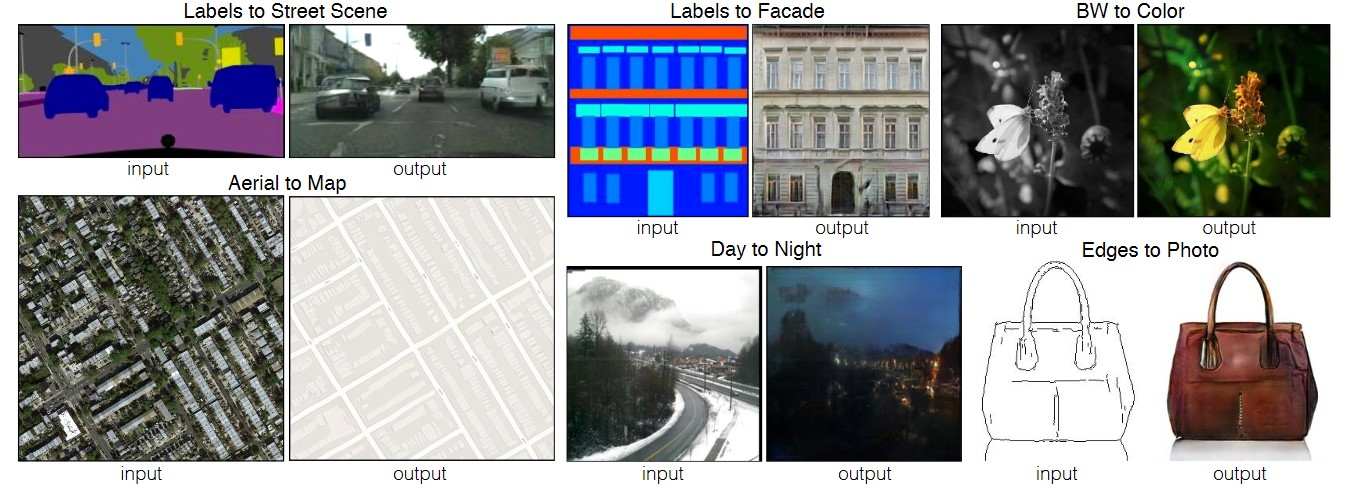
\includegraphics[width=15cm]{images/appofpix2pix.jpg}
\caption{Các ứng dụng của khung mô hình pix2pix \cite{isola2018imagetoimage}.}
\label{fig:appofpix2pix}
\end{figure}

Vô số các ứng dụng liên quan đã được tạo ra (hình \ref{fig:appofpix2pix}), tiêu biểu như:

\begin{itemize}
    \item Chuyển đổi trời tối sang trời sáng.
    \item Tái tạo phong cách hội hoạ của những hoạ sĩ nổi tiếng đã qua đời như Van Gogh, Picasso, Monet,... dựa trên những bức tranh họ để lại.
    \item Chuyển đổi từ ảnh được phân vùng sang ảnh thật.
    \item Thêm màu sắc cho các nét vẽ để tạo thành ảnh màu hoàn chỉnh.
    \item Tạo màu cho ảnh xám.
    \item Hay một ứng dụng tuyệt vời nhất mà được chúng ta sử dụng hằng ngày, đó chính là chuyển đổi bức ảnh chụp từ vệ sinh sang Google Maps.
\end{itemize}

Đồ án này triển khai một mô hình dựa theo khung mô hình pix2pix để giải quyết bài toán tạo màu cho ảnh xám.
Một ứng dụng của khung mô hình trên.
Kích thước ảnh được chọn để xử lý sẽ là $256 \times 256$, một kích thước phổ biến trong những mạng tích chập hiện nay và phù hợp cho mô hình được triển khai.

\section{Phát biểu bài toán, cách áp dụng vào khung mô hình pix2pix và hàm mất mát}

Bài toán tạo màu có thể được phát biểu như sau:

\begin{tcolorbox}
Cho một ảnh xám đầu vào $\mathcal{I}_{\text{đầu vào}} \in \bm{G}_{\mathbf{L}^*}^{256 \times 256}$, ta cần xây dựng một ánh xạ:
\begin{align}
    \mathcal{G}&: \bm{G}_{\mathbf{L}^*}^{256 \times 256} \rightarrow \left(\bm{G}_{\mathbf{a}^*} \times \bm{G}_{\mathbf{b}^*}\right)^{256 \times 256}\\
    \widehat{\mathcal{I}} &= \left(\mathcal{I}_{\text{đầu vào}}, \mathcal{G}\left(\mathcal{I}_{\text{đầu vào}}\right)\right) \in \left(\bm{G}_{\mathbf{L^*}\mathbf{a^*}\mathbf{b^*}}\right)^{256 \times 256}\label{eqn:fakeimage}
\end{align}

Sao cho ảnh $\widehat{\mathcal{I}}$ (\ref{eqn:fakeimage}) là một ảnh màu trong không gian màu \textbf{L*a*b*} có được sự hợp lí, chân thực với mắt người.\vspace{5pt}

Việc xây dựng ánh xạ sẽ được dẫn đường bởi ánh xạ:
\begin{align}
    \mathcal{D}:\left(\bm{G}_{\mathbf{L^*}\mathbf{a^*}\mathbf{b^*}}\right)^{256 \times 256} \rightarrow \mathbb{R}^{70 \times 70}
\end{align}

\end{tcolorbox}

Trong mạng GAN pix2pix được huấn luyện, bộ sinh $G$ sẽ là ánh xạ $\mathcal{G}$ cần tìm.
Còn ánh xạ $\mathcal{D}$ là bộ phân biệt $D$ có nhiệm vụ phân biệt ảnh màu đưa vào là thật hay giả, hỗ trợ xây dựng ánh xạ $\mathcal{G}$.\vspace{5pt}

Bộ sinh theo kiến trúc mạng Unet với đầu vào là một ảnh $\mathcal{I}_{\text{đầu vào}}$ chỉ có một kênh biểu thị cho cường độ sáng mỗi điểm ảnh.
Bức ảnh sẽ được truyền vào một kiến trúc mạng tích chập để trích lọc đặc trưng thông qua quá trình mã hoá.
Ở quá trình này, kích thước đầu ra ở mỗi tầng sẽ giảm dần theo bội 2.
Trong giai đoạn giải mã, các đặc trưng được kết hợp với phía trái nhánh chữ U là phần mã hoá, để biến đổi lại thành ảnh đích bằng tích chập chuyển vị.
Và mỗi tầng sẽ có kích thước tăng dần cũng theo bội 2.
Kết quả trả ra sau cùng là hai kênh màu $\widehat{\mathcal{I}}_{\text{đầu ra}} = \mathcal{G}\left(\mathcal{I}_{\text{đầu vào}}\right)$.
Khi đó, ảnh giả được bộ sinh tạo ra là $\widehat{\mathcal{I}} = \left(\mathcal{I}_{\text{đầu vào}}, \widehat{\mathcal{I}}_{\text{đầu ra}}\right)$.\vspace{5pt}

Đầu vào của bộ phân biệt có thể là ảnh $\mathcal{I} = \left(\mathcal{I}_{\text{đầu vào}}, \mathcal{I}_{\text{đầu ra}}\right)$ với $\mathcal{I}_{\text{đầu ra}} \in \bm{G}_{\mathbf{a}^*} \times \bm{G}_{\mathbf{b}^*}$ là nhãn tương ứng với $\mathcal{I}_{\text{đầu vào}}$ trong tập dữ liệu huấn luyện.
Với đầu vào này, ta sẽ gán nhãn cho là $\mathbf{P_D} = \mathbf{J}_{70 \times 70}$ vì là dữ liệu thật.
Còn khi dữ liệu đầu vào là $\widehat{\mathcal{I}}$, ta sẽ có nhãn cho bộ phân biệt là $\mathbf{P_D} = \mathbf{O}_{70 \times 70}$.\vspace{5pt}

Dựa vào (\ref{eqn:losspix2pix}) và bỏ nhiễu [\textbf{\ref{objofpix2pix}}], ta có hàm mục tiêu cho bài toán tô màu là:
\begin{align}
    \mathcal{G}^* = \arg\min_{\mathcal{G}}\max_{\mathcal{D}}\bigl\{
    \mathbb{E}_{\mathcal{I}}\left[\log \mathcal{D}\left(\mathcal{I}\right)\right]
    &+ \mathbb{E}_{\mathcal{I}_{\text{đầu vào}}}\left[\log\left(1-\mathcal{D}\left(\mathcal{I}_{\text{đầu vào}}, \mathcal{G}\left(\mathcal{I}_{\text{đầu vào}}\right)\right)\right)\right] \nonumber\\
    &+ \lambda \underbrace{\mathbb{E}_{\mathcal{I}_{\text{đầu vào}}, \mathcal{I}_{\text{đầu ra}}}\lVert \mathcal{I}_{\text{đầu ra}} - \mathcal{G}\left(\mathcal{I}_{\text{đầu vào}}\right)\rVert}_{\mathcal{L}_{L1}\left(\mathcal{G}\right)}\bigr\}\label{eqn:lossofmainmodal}
\end{align}

Hệ số $\lambda$ được chọn giống như \cite{isola2018imagetoimage} gợi ý là $\lambda = 100$.\vspace{5pt}

\section{Kiến trúc bộ sinh pix2pix và bộ sinh học chuyển giao từ xương sống ResNet18}\label{transferlearning}

Trong mô hình tạo màu, được quan tâm hơn cả là bộ sinh vì nó là ánh xạ $\mathcal{G}$ ta cần tìm để giải bài toán tạo màu.
Kiến trúc tổng quát bộ sinh được đề xuất trong \cite{isola2018imagetoimage} như sau:
\begin{align}
    &\text{nhánh trái:} \text{I} \rightarrow \text{C64} \rightarrow \text{C128} \rightarrow \text{C256} \rightarrow \text{C512} \rightarrow \text{C512} \rightarrow \text{C512} \rightarrow \text{C512} \rightarrow \text{C512}\\
    &\text{nhánh phải:} \rightarrow \text{D512} \rightarrow \text{D1024} \rightarrow \text{D1024} \rightarrow \text{D1024} \rightarrow \text{D512} \rightarrow \text{D256} \rightarrow \text{D128} \rightarrow \text{D2}
\end{align}

Trong đó, $\text{Ck}$ là một tầng tích chập $k$ bộ lọc, $\text{Dk}$ là một tầng giải chập bằng tích chập chuyển vị với $k$ bộ lọc.
Cả 2 quá trình chập và giải chập đều sử dụng kích thước bộ lọc là $4$, sải bước $2$ và đệm $1$.\vspace{5pt}

Xây dựng mô hình theo kiến trúc trên không quá khó.
Nhưng huấn luyện để có được kết quả tốt tương tự, khi hạn chế về số lượng và chất lượng của tập dữ liệu, cũng như phần cứng máy tính bị giới là khá thử thách [\textbf{\ref{badexperiment}}].\vspace{5pt}

Cải thiện mô hình mà vẫn tiết kiệm chi phí, phương pháp học chuyển giao được áp dụng để làm điều này.
Kiến trúc cho bộ sinh vẫn sẽ là kiến trúc theo mạng Unet, tuy nhiên sẽ được chuyển giao bằng cách lấy xương sống là ResNet18 \cite{christopherresunet2019}.
Có 3 họ mạng được chủ yếu dùng để làm xương sống cho Unet là VGG, ResNet và Xception \cite{backboneresnet2020}.
Trong những họ mạng trên, ResNet18 thuộc họ mạng ResNet có kích thước không quá lớn \cite{Khan_2020}, phù hợp để huấn luyện với phần cứng bị giới hạn.

\begin{figure}[!h]
\captionsetup{width=0.8\textwidth}
\centering
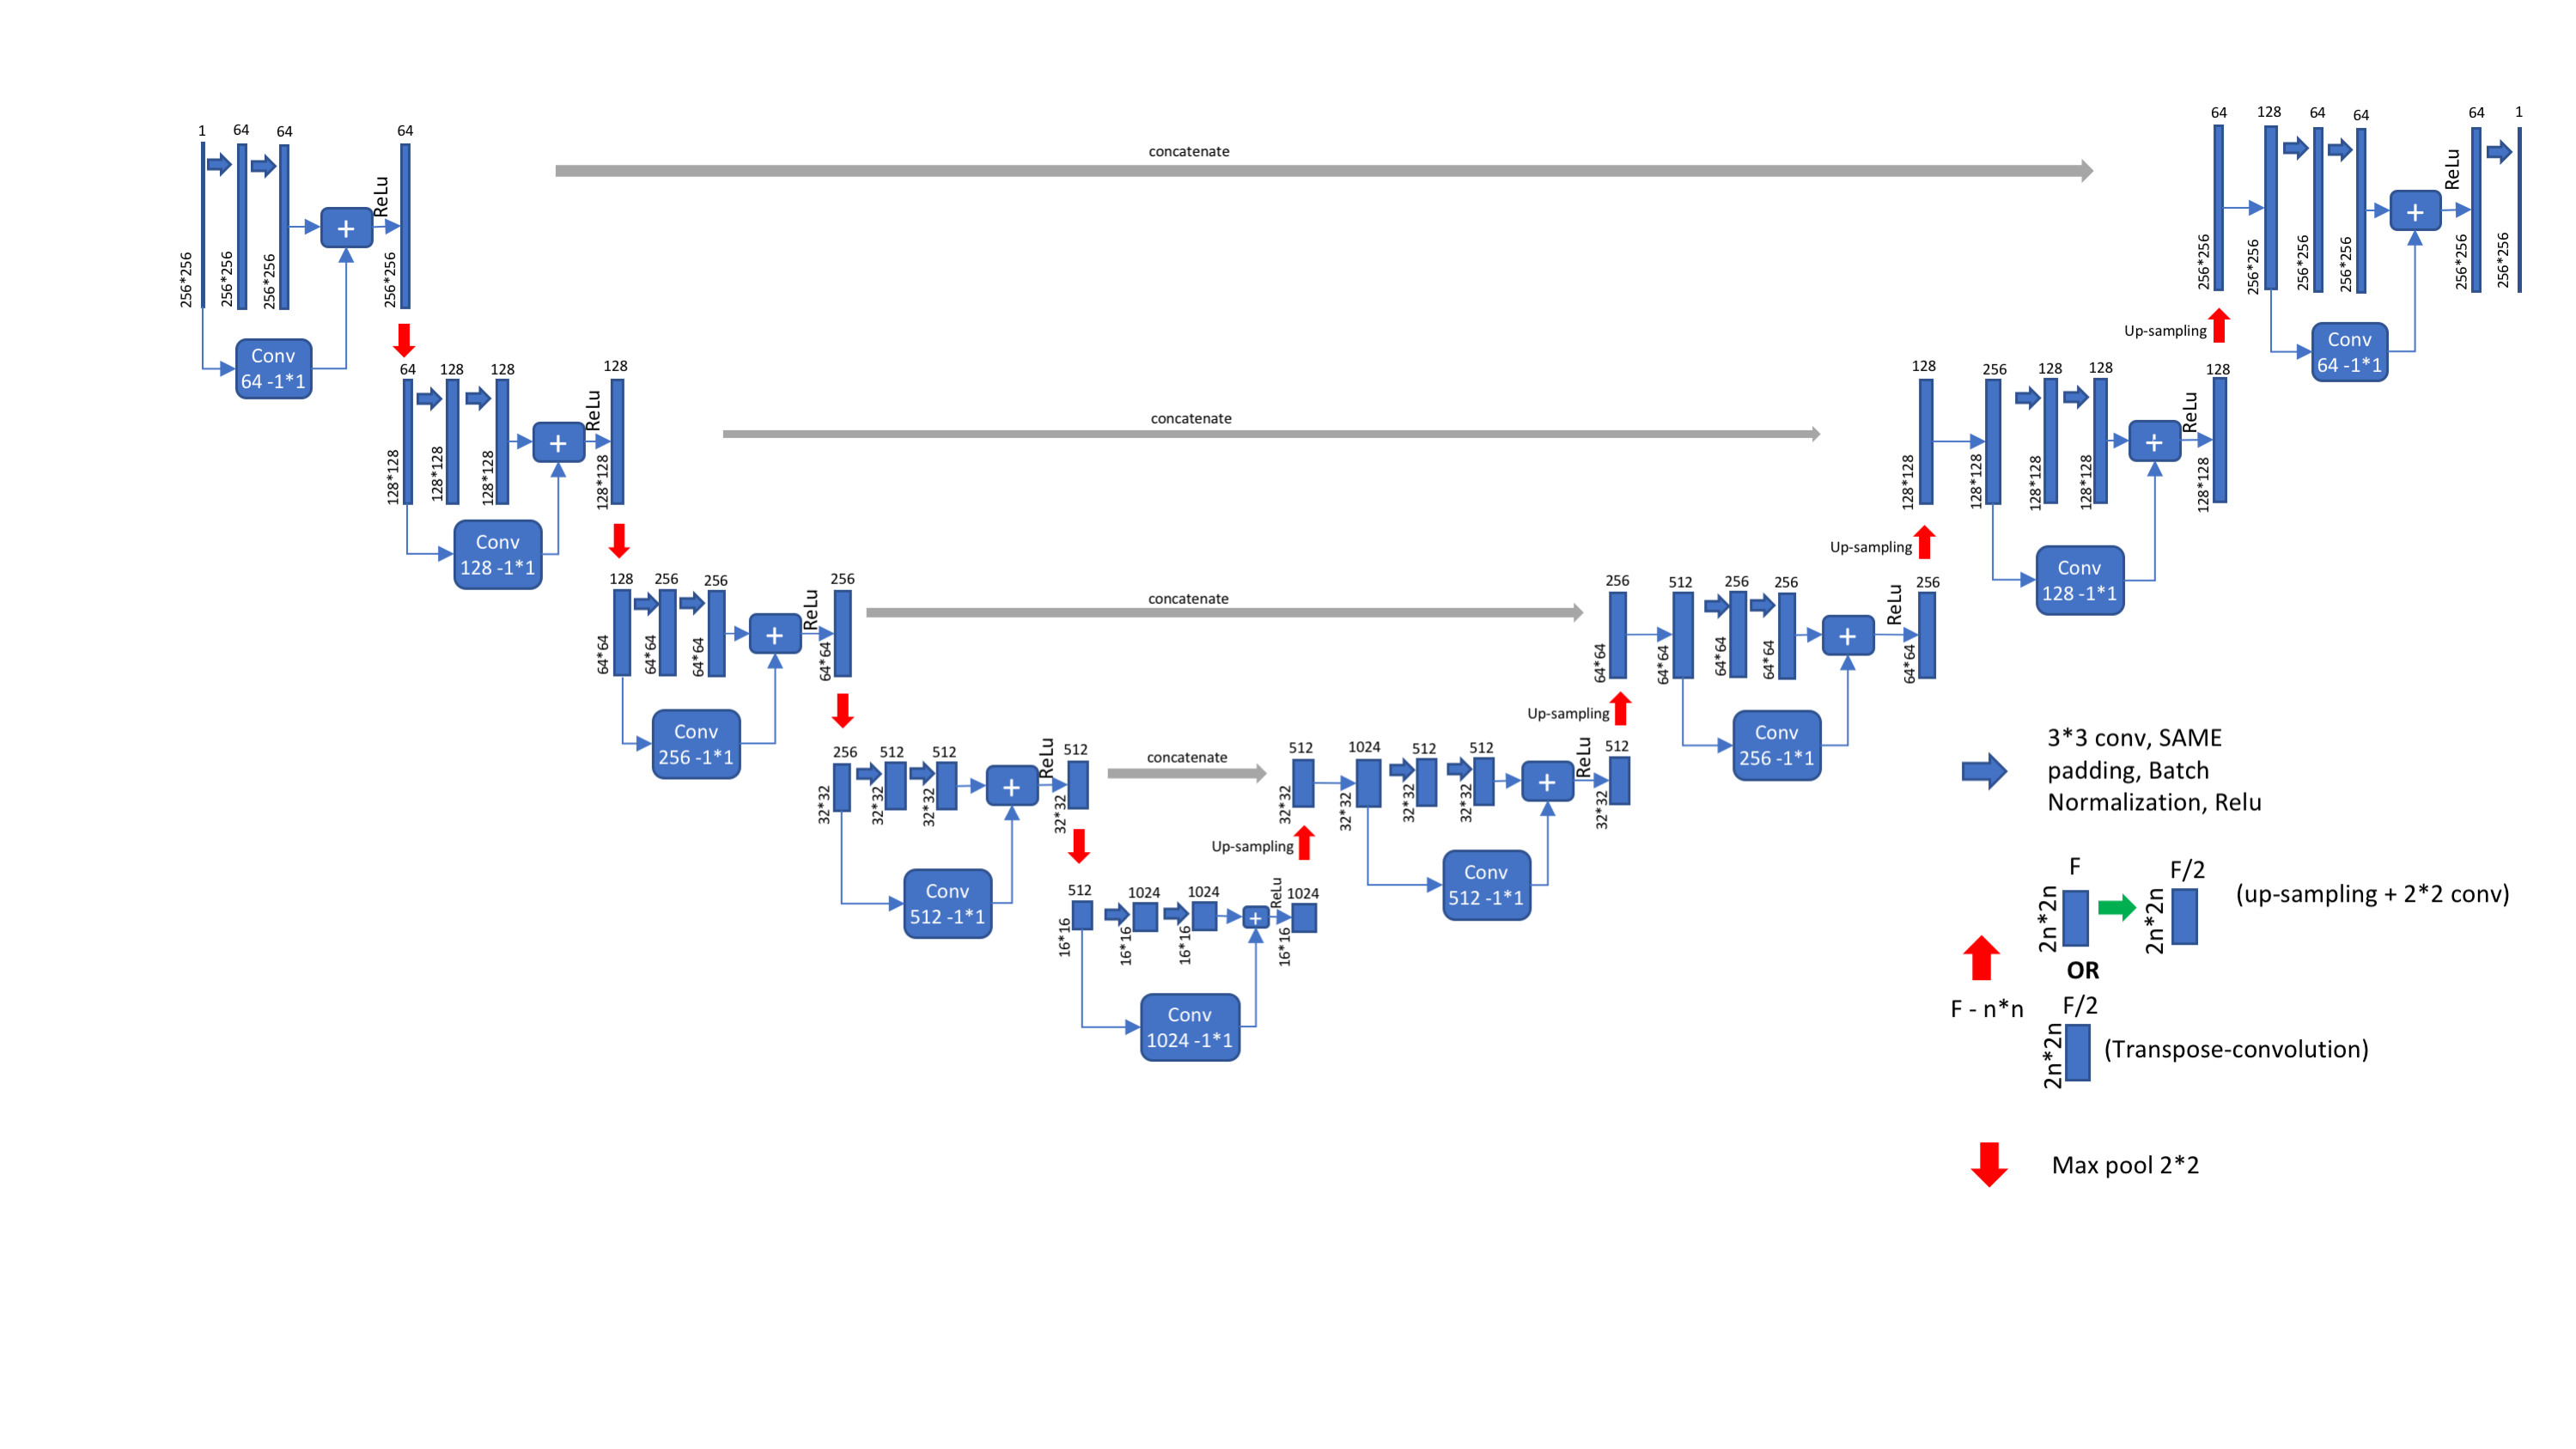
\includegraphics[width=17cm]{images/unetresnet.png}
\caption{Một kiểu mạng Unet được khởi tạo theo phong cách ResNet \cite{unetwithresblocknishank2019}.}
\end{figure}

Một lưu ý là toàn bộ phần tích chập của ResNet18 (đã bỏ đi các tầng kết nối dày đặc) sẽ chỉ làm ở phía mã hoá, tức nhánh bên trái của chữ U chứ không hề xây dựng lên toàn bộ cả mạng Unet.
Phần mã hoá sẽ được tự động khởi tạo thích hợp bởi thư viện fastai\footnote{fastai Documentation, ``Dynamic UNet'', \href{https://docs.fast.ai/vision.models.unet.html}{https://docs.fast.ai/vision.models.unet.html}}.

%%%%%%%%%%%%%%%%%%%%%%%%%%%%%%%%%
\chapter{Triển khai mô hình}\label{implementation}

\section{Ngôn ngữ lập trình và thư viện chính}

Ngôn ngữ lập trình được sử dụng để triển khai mô hình là \textbf{Python} với sự hỗ trợ chính của thư viện \textbf{PyTorch}.
Để cài đặt những công cụ này, có thể theo đường dẫn bên dưới:

\begin{itemize}
    \item Python: \href{https://www.python.org/downloads/}{https://www.python.org/downloads/}
    \item PyTorch \href{https://pytorch.org/get-started/locally/}{https://pytorch.org/get-started/locally/}
\end{itemize}

Thư viện \textbf{fastai} (bản mới nhất) cũng được cài đặt cho việc xây dựng mạng Unet và một số tác vụ liên quan.
Để tải thư viện này về, mở cửa sổ dòng lệnh (đã được nhúng môi trường Python) rồi thực thi mã lệnh:

\begin{lstlisting}
pip install fastai --upgrade
\end{lstlisting}

Toàn bộ mã nguồn, cũng như những tệp liên quan trong quá trình hoàn thành mô hình, có thể tìm thấy trong thư mục đồ án tại:

\begin{itemize}
    \item Github: \href{https://github.com/dee-ex/EE3151\_SEM202\_PROJECT}{https://github.com/dee-ex/EE3151\_SEM202\_PROJECT}
\end{itemize}

Để có thể biết được đầy đủ những thư viện cũng như phiên bản thư viện được sử dụng, tham khảo tệp tin \texttt{requirements.txt} trong đường dẫn thư mục đồ án.

\section{Tập dữ liệu, chuấn hoá và làm giàu dữ liệu}\label{normalization}

Tập dữ liệu được chọn sử dụng là tập \textbf{COCO}\footnote{COCO Dataset - Download, \href{https://cocodataset.org/\#download}{https://cocodataset.org/\#download}} (hình \ref{fig:cocodataset}) có trong thư viện \textbf{fastai}, ta có thể dễ dàng tải về.
Số lượng ảnh được chọn để huấn luyện là $10,000$.
Tất cả đều được chọn ngẫu nhiên và có xáo trộn.

\begin{figure}[!h]
\captionsetup{width=0.8\textwidth}
\centering
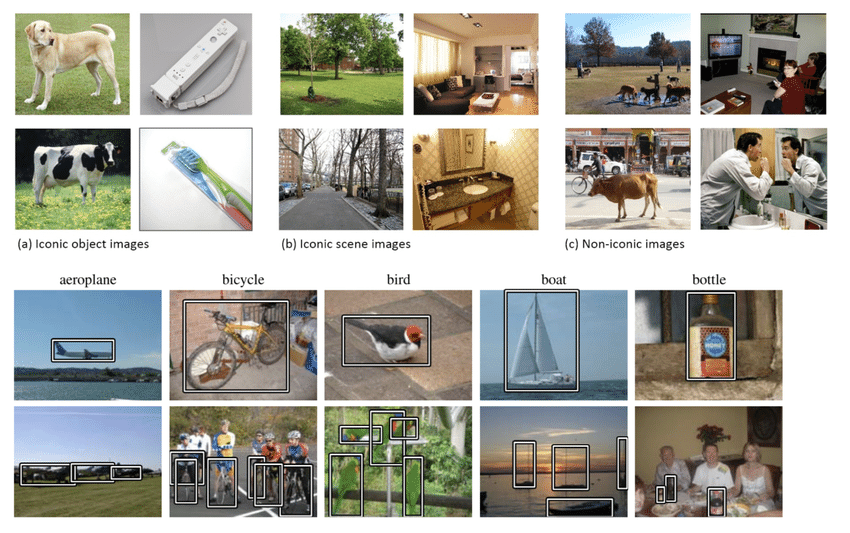
\includegraphics[width=15cm]{images/3_1.png}
\caption{Hình ảnh trích từ tập dữ liệu COCO.}
\label{fig:cocodataset}
\end{figure}

Chuẩn hoá dữ liệu đầu vào là bước tiền xử lí giúp tăng tốc độ hội tụ cho mô hình, giảm sự phụ thuộc của gradient vào tỉ lệ các tham số và một số lợi ích khác \cite{jasonscaledata2019, benscaledata2012}.
Ở đây, 3 kênh dữ liệu sẽ được chuẩn hoá cùng về một khoảng $[-1, 1]$:
\begin{align}
    \bm{G}_{\text{chuẩn hoá } \mathbf{L}^*} &= \dfrac{\bm{G}_{\mathbf{L}^*}}{50} - 1 \label{eqn:normalizelchannel}\\
    \bm{G}_{\text{chuẩn hoá } \mathbf{a}^*} &= \dfrac{\bm{G}_{\mathbf{a}^*}}{110} \label{eqn:normalizeachannel}\\
    \bm{G}_{\text{chuẩn hoá } \mathbf{b}^*} &= \dfrac{\bm{G}_{\mathbf{b}^*}}{110} \label{eqn:normalizebchannel}
\end{align}

Vì $\bm{G}_{\mathbf{L}^*} \in [1, 100]$, nên ta chuẩn hoá như (\ref{eqn:normalizelchannel}) là hết sức bình thường.
Riêng với (\ref{eqn:normalizeachannel}) và (\ref{eqn:normalizebchannel}) lại có thể gây một chút khó hiểu.
Bởi vì thư viện được sử dụng để chuyển đổi màu là \textbf{skimage}.
Và trong \textbf{skimage} thì $\bm{G}_{\mathbf{a}^*} \in [-86, 98]$ và  $\bm{G}_{\mathbf{b}^*} \in [-108, 94]$ \cite{replyrangelabinskimage2020}.
Do đó, cận trên $110$ để chuẩn hoá.
Ta cũng hoàn toàn có thể chọn riêng cận trên để chuẩn hoá.
Giả sử như của $\bm{G}_{\mathbf{a}^*}$ là $100$, còn $\bm{G}_{\mathbf{b}^*}$ là $110$.
Dĩ nhiên, trong cả hai hướng chuẩn hoá trên thì một số trường hợp khi đưa từ giá trị chuẩn hoá về lại giá trị gốc, sẽ không còn khớp với thư viện \textbf{skimage}.
Tuy nhiên, phần đó là thiểu số, không quá đáng kể.\vspace{5pt}

Bên cạnh chuẩn hoá không gian màu, kích thước ảnh cũng sẽ được điều chỉnh lại thành ảnh vuông kích thước $256\times 256$ nếu cần thiết.
Sử dụng lật đối xứng theo trục tung (hình \ref{fig:horizontalflip}) để làm giàu dữ liệu cho việc huấn luyện.
Như vậy, tổng số lượng dữ liệu mà mô hình được học sẽ là $10,000 \times 2 = 20,000$.

\begin{figure}[!h]
\captionsetup{width=0.8\textwidth}
\centering
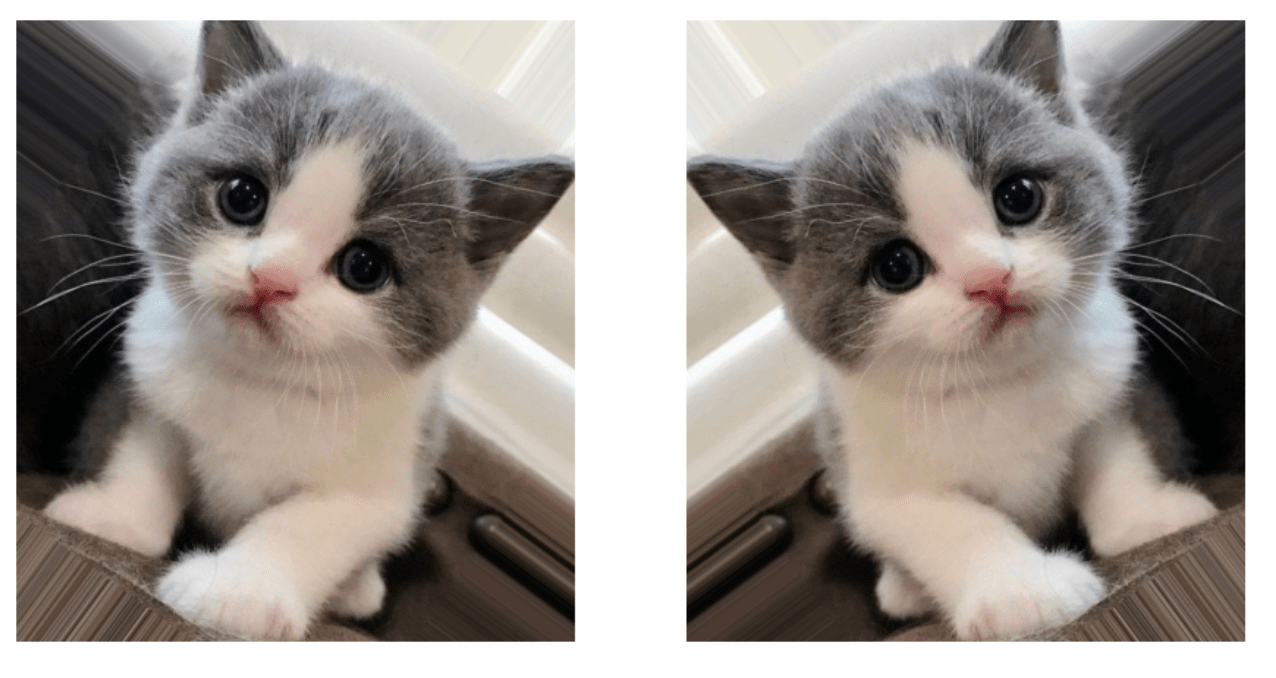
\includegraphics[width=15cm]{images/horizontalflip.png}
\caption{Minh hoạ việc lật đối xứng theo trục tung.}
\label{fig:horizontalflip}
\end{figure}

\section{Huấn luyện mô hình}

Cách thức huấn luyện cho mô hình pix2pix sử dụng Python-PyTorch được tham khảo chính từ \cite{aladdinperssonyoutube, moeincolorization2020, junyanzho2020}.
Đồng thời cũng có thêm một vài tham khảo về việc sử dụng Keras \cite{tuannguyenpix2pix2020, khanhpix2pix2020, jasonpix2pix2019} để huấn luyện những mô hình tương tự.\vspace{5pt}

Vì mô hình bộ sinh phức tạp và quan trọng hơn so với bộ phân biệt, vậy nên để cho quá trình huấn luyện GAN được ổn định hơn, cũng như tránh bộ phân biệt hội tụ sớm, ta sẽ tiền huấn luyện \cite{ham2020unbalanced} độc lập bộ sinh bằng $\mathcal{L}_{L1}\left(\mathcal{G}\right)$ (\ref{eqn:lossofmainmodal}) qua 20 epoch với kích thước batch là 16.
Mỗi epoch mất khoảng 6--7 phút khi huấn luyện trên Google Colab\footnote{Google Colab, \href{https://colab.research.google.com/}{https://colab.research.google.com/}}.
Thuật toán tối ưu được sử dụng là Adam \cite{kingma2017adam} với tốc độ học $\alpha = 10^{-4}$ và mô men $\beta_1 = 0.9, \beta_2=0.999$.\vspace{5pt}

\begin{figure}[!h]
\captionsetup{width=0.8\textwidth}
\centering
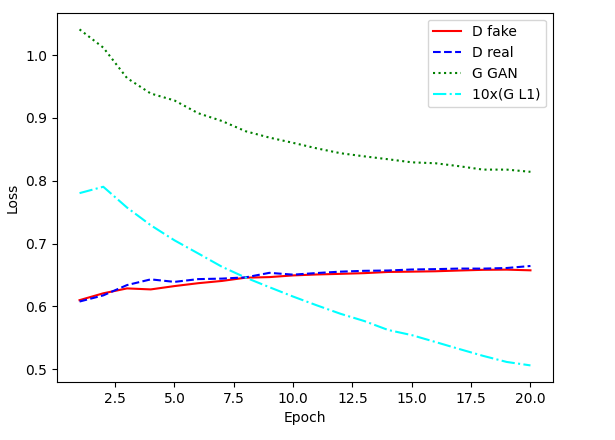
\includegraphics[width=15cm]{images/3_6.png}
\caption{Giá trị các thành phần mất mát của bộ phân biệt và bộ sinh qua từng epoch.}
\label{fig:losstrainning}
\end{figure}

Tải các thông số của bộ sinh đã được tiền huấn luyện độc lập trước đó, đưa vào quá trình huấn luyện một mạng đối nghịch.
Thuật toán tối ưu vẫn sẽ dùng là Adam với tốc độ học $\alpha=2.10^{-4}$ và mô men $\beta_1 = 0.5, \beta_2=0.999$.
Mô hình được huấn luyện qua 20 epoch với kích thước batch là 16.
Các batch sẽ có số chiều là $16 \times 1 \times 256 \times 256$ (kích thước batch, số kênh, số hàng, số cột).
Mỗi epoch mất khoảng 10--16 phút bằng việc sử dụng Google Colab để thực thi.\vspace{5pt}

Nhận thấy xu hướng của giá trị mất mát khi huấn luyện mô hình GAN (hình \ref{fig:losstrainning}) là: giá trị mất mát của bộ phân biệt (đường nét liền đỏ và đường nét đứt lam) tăng thì giá trị mất mát của bộ sinh (đường nét chấm lục) sẽ giảm.
Điều này khá dễ dàng để lý giải.
Khi bộ phân biệt đạt đến một ngưỡng thông minh nhất định, bộ sinh thì lại càng thông minh qua mỗi epoch, hiển nhiên sẽ đánh lừa được bộ phân biệt.
Chuyện này là hợp lí với nguyên lí non-zero-sum-games.
Ngoài ra, giá trị mất mát của bộ sinh theo chuẩn 1 (đường nét chấm đứt xanh ngọc) cũng được giảm, tuy không đáng kể so với những mất mát còn lại.\vspace{5pt}

Tuy hợp lí là thế, nhưng mô hình kiểu GAN khá khó để nói trước ngoài việc xem xét kết quả thử nghiệm.
Sau một số thử nghiệm định tính đơn giản, mô hình có kết quả tốt nhất theo quan điểm chủ quan là mô hình sau epoch thứ 15\footnote{Tất cả 20 mô hình qua mỗi epoch đều được lưu giữ lại trong thư mục đồ án tại đường dẫn \href{https://github.com/dee-ex/EE3151\_SEM202\_PROJECT/tree/main/training_results/GAN_models}{./training\_results/GAN\_models}}.
Và sẽ là lựa chọn cho các thử nghiệm và đánh giá trong những phần sau.

%%%%%%%%%%%%%%%%%%%%%%%%%%%%%%%%%
\chapter{Thử nghiệm và đánh giá mô hình}\label{testmodel}

\section{Mô hình GAN với bộ sinh kiến trúc pix2pix}\label{badexperiment}

Kết quả ở hình dưới là kết quả của mô hình với bộ sinh xây dựng theo kiến trúc đề xuất của tác giả pix2pix [\textbf{\ref{transferlearning}}], được thử nghiệm với 5 bức ảnh ngẫu nhiên lấy từ tập COCO (không nằm trong tập huấn luyện).
Khá không may mắn, kết quả không được như chúng ta mong đợi (hình \ref{fig:worseexperiment}).

\begin{figure}[!h]
\captionsetup{width=0.8\textwidth}
\centering
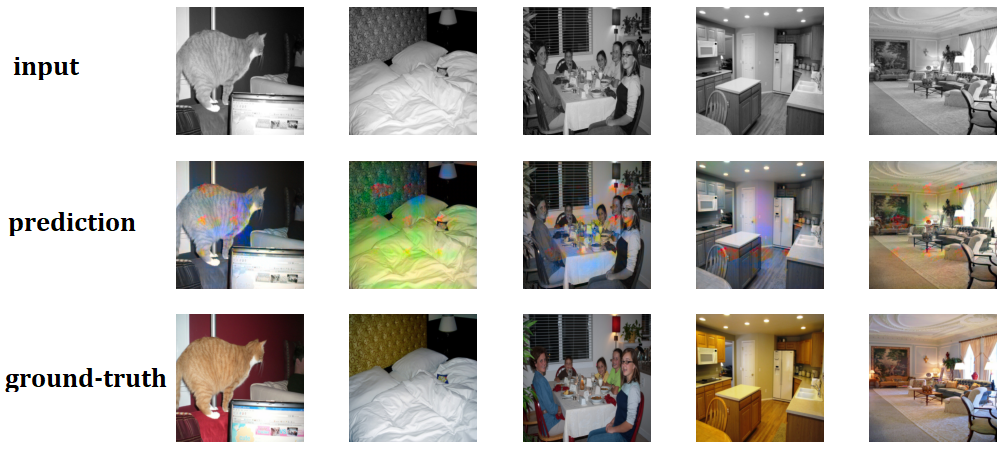
\includegraphics[width=15cm]{images/4_0.png}
\caption{Kết quả dự đoán của mô hình GAN với bộ sinh đơn giản sau epoch thứ 34 trên tập dữ liệu COCO.}
\label{fig:worseexperiment}
\end{figure}

Nhìn chung, việc huấn luyện mô hình là khả thi khi mô hình cũng đã có thể tạo được màu cho một số điểm ảnh (hình \ref{fig:worseexperiment} ở vị trí phía phải ngoài cùng) sau vài chục epoch.
Nhưng như đã nêu ra [\textbf{\ref{transferlearning}}], giới hạn về phần cứng cũng như là tập dữ liệu không đủ nhiều và tốt, để có thể huấn luyện được mô hình theo như mong đợi.\vspace{5pt}

Nhìn thêm ở một góc độ khác, việc huấn luyện một mạng GAN cũng không hề dễ dàng, khi GAN rất dễ bị nhạy cảm với những thông số được cài đặt khi huấn luyện \cite{hard2trainganjonathan2018}.
Sau nhiều lần thử nghiệm thất bại, một trong số những kinh nghiệm rút ra là, trong hầu hết các mô hình GAN, ta nên khởi tạo các trọng số của mô hình và bias theo phân phối $\mathcal{N}\left(\mu, \sigma^2\right) = \mathcal{N}\left(0, 0.1\right)$ để quá trình huấn luyện nhanh hội tụ hơn.
Dĩ nhiên không thể thiếu một điều kiện cần là một tập dữ liệu có chất lượng tốt.

\section{Mô hình GAN với bộ sinh có xương sống ResNet18}

\begin{figure}[!h]
\captionsetup{width=0.8\textwidth}
\centering
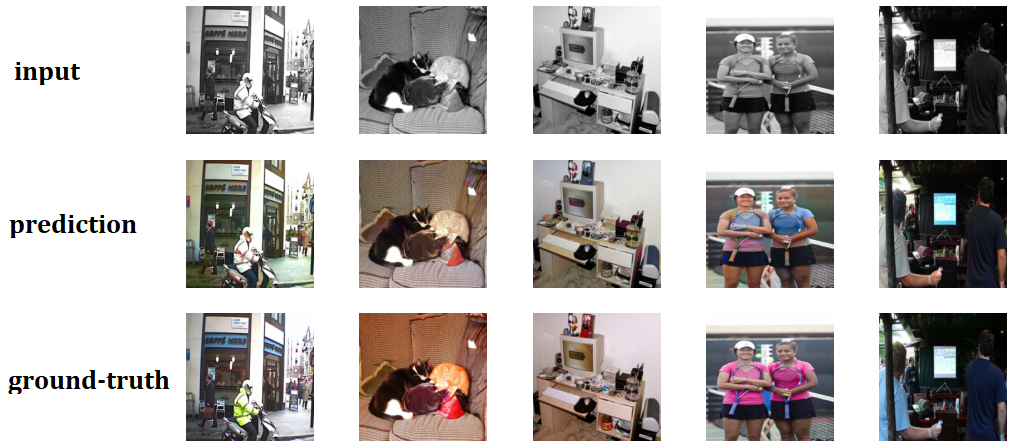
\includegraphics[width=15cm]{images/4_1.png}
\caption{Kết quả dự đoán của mô hình GAN với bộ sinh đơn giản có xương sống ResNet18 sau epoch thứ 15 trên tập dữ liệu COCO (không nằm trong tập huấn luyện).}
\label{fig:betterexperiment}
\end{figure}

\noindent
Kết quả ở hình \ref{fig:betterexperiment} dễ thấy đã cải thiện hơn hẳn so với kết quả ở hình \ref{fig:worseexperiment}.
Màu tạo ra ít bị lem hay lộn xộn như kết quả [\textbf{\ref{badexperiment}}].
Một vài đối tượng có màu khác với màu của ảnh gốc, ví dụ người lái xe ở ảnh phía trái ngoài cùng, nhưng vẫn hết sức hợp lí và tự nhiên.\vspace{5pt}

Ở một số vùng ảnh, mô hình có vẻ như vẫn chưa thực sự chọn được màu phù hợp và rồi để màu gần giống với mức xám ban đầu.
Có thể là do những vùng chưa có màu hợp lí là trong quá trình huấn luyện, mô hình chưa được học qua ảnh có đặc trưng, đối tượng tương tự.

\begin{figure}[!h]
\captionsetup{width=0.8\textwidth}
\centering
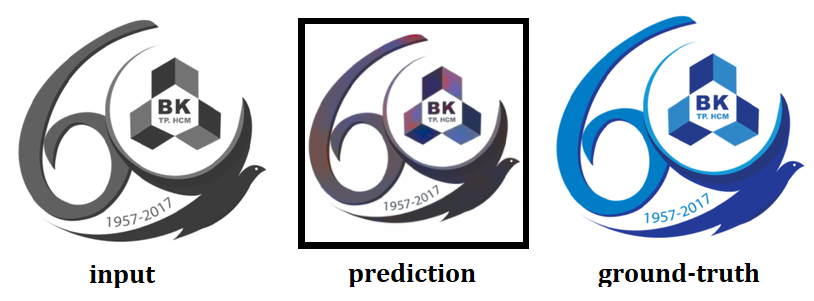
\includegraphics[width=15cm]{images/4_12.PNG}
\caption{Mô hình hoàn toàn bế tắc trước logo kỷ niệm 60 năm của trường ĐH Bách Khoa TP.HCM.}
\label{fig:failcolorlogo}
\end{figure}

\begin{figure}[!h]
\captionsetup{width=0.8\textwidth}
\centering
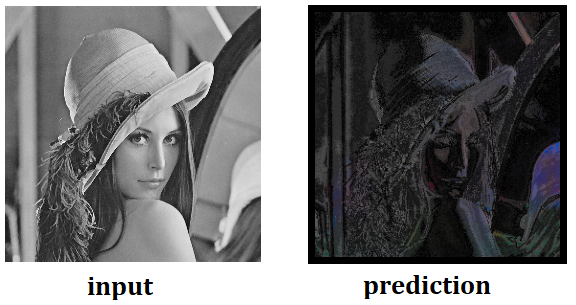
\includegraphics[width=15cm]{images/4_13.png}
\caption{Trường hợp đặc biệt khi mô hình làm việc tệ với ảnh có đặc trưng đơn giản.}
\label{fig:edgecase}
\end{figure}

Điều trên dẫn đến một hạn chế khác nữa là đối với những ảnh không có đặc trưng rõ ràng, những đặc trưng lạ lẫm mà chưa được đưa vào huấn luyện cho mô hình.
Chẳng hạn ảnh chủ đề logo (hình \ref{fig:failcolorlogo}), mô hình hoàn toàn không có khả năng tạo được màu phù hợp vì không hiểu được đặc trưng.\vspace{5pt}

Thêm một hạn chế khác là mô hình cũng chưa thực sự biết được những điểm ảnh nào sẽ cùng một đối tượng và cùng màu.
Cụ thể như trong hình \ref{fig:betterexperiment}, ảnh hai cố gái cầm vợt tennis (thứ 2 từ phía bên phải), phần dưới của áo được chọn là màu hồng, còn phần trên của áo lại màu xanh.
Nếu mô hình lựa cho phần áo màu hồng hay màu xanh thì đều chấp nhận được, nhưng mô hình lại chọn cách lựa hai phía của áo bởi hai màu khác nhau không đồng nhất.\vspace{5pt}

Riêng với trường hợp hình \ref{fig:edgecase} thực sự là một kết quả bất ngờ, mà hiện tại vẫn chưa tìm ra lí do thích hợp cho việc mô hình cho kết quả không thực sự tốt.
Việc mô hình không có khả năng làm việc với đặc trưng mặt người là không khả thi, khi [\textbf{\ref{compare}}, \textbf{\ref{surveyforevaluation}}] cũng có các ảnh mặt người tương tự và mô hình vẫn cho kết quả ổn.
Đây là một trường hợp đặc biệt cần thêm nhiều tìm hiểu.

\section{So sánh bộ sinh có xương sống ResNet18 trước và sau khi huấn luyện đối nghịch}\label{compare}

Việc so sánh mô hình bộ sinh trước (bộ sinh đã được qua tiền huấn luyện đối lập) và sau khi huấn luyện đối nghịch cùng bộ phân biệt, sẽ cho ta thấy hiệu quả của huấn luyện kiểu GAN mang lại.
Một số ảnh đen trắng (hình \ref{fig:sampletotest}) được lựa chọn gồm các bối cảnh chân dung, phong cảnh, toà nhà cũng như những ảnh có nhiều đối tượng (chi tiết) để thử nghiệm.

\begin{figure}[!h]
\captionsetup{width=0.8\textwidth}
\centering
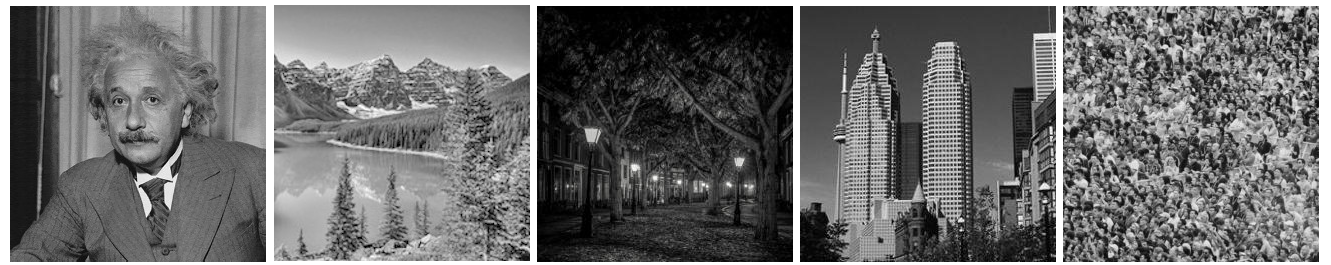
\includegraphics[width=15cm]{images/4_2.PNG}
\caption{Những tấm ảnh đen trắng được lựa chọn để so sánh sự khác biệt.}
\label{fig:sampletotest}
\end{figure}

Trước khi đưa cho mô hình thực hiện tạo màu, không khó để đoán được rằng hình ảnh đầu tiên (phía trái ngoài cùng) có ít chi tiết nhất nên khả năng cao sẽ có kết quả tốt nhất.
Ngược lại, hình ảnh cuối cùng (phía phải ngoài cùng) có rất nhiều chi tiết nên kết quả cũng rất có thể không đạt được tốt như những tấm ảnh ít chi tiết.
Và quả thật không ngoài dự đoán, kết quả có được khá đúng với những gì mong đợi.

\begin{figure}[!h]
\captionsetup{width=0.8\textwidth}
\centering
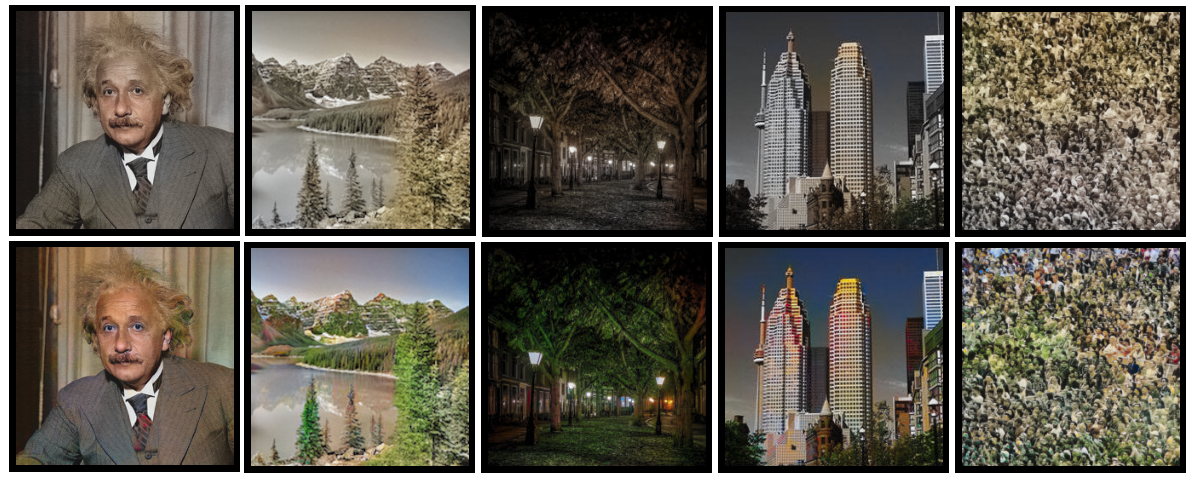
\includegraphics[width=15cm]{images/4_3.PNG}
\caption{Phía trên và dưới lần lượt là kết quả của bộ sinh trước và sau khi huấn luyện đối nghịch.}
\label{fig:comparesimpleandgan}
\end{figure}


Ta có thể thấy trong hình \ref{fig:comparesimpleandgan} một điều là, mô hình sau khi được huấn luyện theo kiểu GAN cho kết quả có màu tươi sáng, chân thật hơn so với khi chưa được uốn nắn bởi bộ phân biệt.
Kết quả đã cải thiện một cách rõ rệt, nên khó có thể nói là mô hình đối nghịch trong mạng GAN không có đóng góp mà chỉ do bộ sinh đã được huấn luyện thêm.\vspace{5pt}

Điểm yếu của việc áp dụng đơn giản hàm mất mát so sánh sai lệch giữa các điểm ảnh, bằng cách dùng chuẩn bậc 1 hoặc bậc 2 như thông thường, đối với bài toán tạo màu rất khó để có kết quả tốt.
Vì mô hình lúc này được khuyến khích để dùng màu xám \cite{zhangcolorization}.
Rõ nghĩa hơn, mô hình đã học được một quy tắc, khi không chắc chắn nên chọn màu gì, thì chọn một giá trị trung bình trong thang $[-1, 1]$ là $\approx (0, 0)$ là một cách an toàn nhất để có thể tối thiểu sai số.
Dẫn đến màu tạo ra có xu hướng không khác là mấy so với màu xám.
Và dĩ nhiên màu trong cuộc sống của chúng ta rất nhiều màu sặc sỡ hơn màu xám.
Khiến cho kết quả của mô hình trước khi đưa vào mạng GAN huấn luyện chưa đáp ứng mục tiêu hợp lí, chân thực đưa ra.

\section{Khảo sát đánh giá định tính chất lượng mô hình}\label{surveyforevaluation}

Với nhiều bài toán liên quan về đồ hoạ, hình ảnh điển hình như bài toán tạo màu, một bài toán có nhiều lời giải thì một trong những bài kiểm tra tốt nhất là kiểm tra dưới góc độ của thị giác con người.
Một cuộc khảo sát (hình \ref{fig:dessurvey}) đã được tiến hành bởi sự giúp đỡ của 100 người, bao gồm những sinh viên thuộc cũng như không thuộc Đại học Quốc gia và một số học sinh cấp trung học phổ thông.
Bài kiểm tra đánh giá bao gồm 20 bức ảnh như trong hình \ref{fig:moreresults} và hình \ref{fig:onemoreresults}, được đánh số thứ tự từ trái sang phải, trên xuống dưới.
Thang điểm đưa ra là từ 1 (rất giả) tới 5 (rất thật).
Trong phần đánh giá, chỉ có ảnh sau khi tạo màu - ảnh ở hàng thứ hai, để tránh thiên lệch khi đánh giá từ người tham gia (hình \ref{fig:questionsurvey}).\vspace{5pt}

Bảng \ref{tab:surveyresults} là kết quả bình chọn từ khảo sát 100 người.
Không quá khó khăn để tính được điểm trung bình mà một tấm ảnh nhận được, bằng cách lấy tổng của số lượt bình chọn nhân với thang điểm tương ứng, rồi chia cho tổng số bình chọn (ở đây là 100).
Kết quả tính toán trên được cho ở bảng \ref{tab:statsurvey}.\vspace{5pt}

Trong những ảnh được bình chọn, ảnh có số điểm cao nhất là ảnh \textbf{05} với số điểm trung bình là \textbf{4.01} (mức 4/5).
Theo sau đó là những ảnh có số điểm 3.96 (07) và 3.94 (09) (hình \ref{fig:besttests}).
Còn ảnh có số điểm trung bình thấp nhất là ảnh \textbf{02} với \textbf{2.53} (mức 2--3/5).
Ngay phía trên là những ảnh có số điểm 2.75 (15) và 2.76 (20) (hình \ref{fig:worsttests}).
Điểm trung bình của 20 bức ảnh khảo sát là \textbf{3.38} (mức 3) và có \textbf{11 (55\%)} ảnh có số điểm trung bình ở trên mức này.\vspace{5pt}

Một điều dễ nhận ra là những ảnh có cây cối, phong cảnh thiên nhiên sẽ là những ảnh có điểm khá cao, từ mức 3 tới mức 5.
Và 2 trong số 3 bức ảnh đạt số điểm cao nhất cũng đều có đặc trưng như trên.
Duy chỉ với ảnh 20, khi có phần tô lem nên đã bị đánh giá thấp đi nhiều, dẫu những phần còn lại có kết quả màu được tạo ra rất đẹp.
Với những ảnh động vật thì kết quả không được khả quan như vậy.
Một trong số đó có kết quả gần tệ nhất là ảnh 15.
Chỉ riêng mỗi ảnh 03 có số điểm khá vượt trội so với những ảnh cùng đặc trưng.
Với đặc trưng về con người, nếu không có quá nhiều chi tiết thì mô hình thể hiện khá tốt và cho số điểm rất cao (3.86 cho ảnh 08 và 3.94 cho ảnh 09).
Nhưng với nhiều chi tiết thì mô hình lại không giữ được phong độ và cho kết quả cực kì tệ, như ảnh 16 với số điểm 2.91 và ảnh 02 với số điểm thấp nhất trong 20 bức ảnh khảo sát.

\begin{figure}[!h]
\captionsetup{width=0.8\textwidth}
\centering
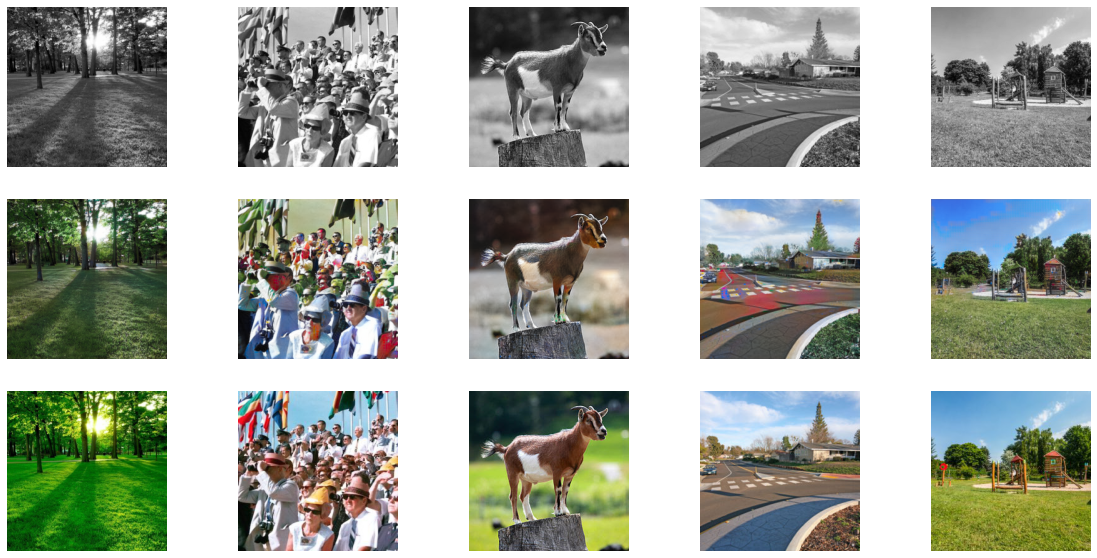
\includegraphics[width=15cm]{images/demo1.png}
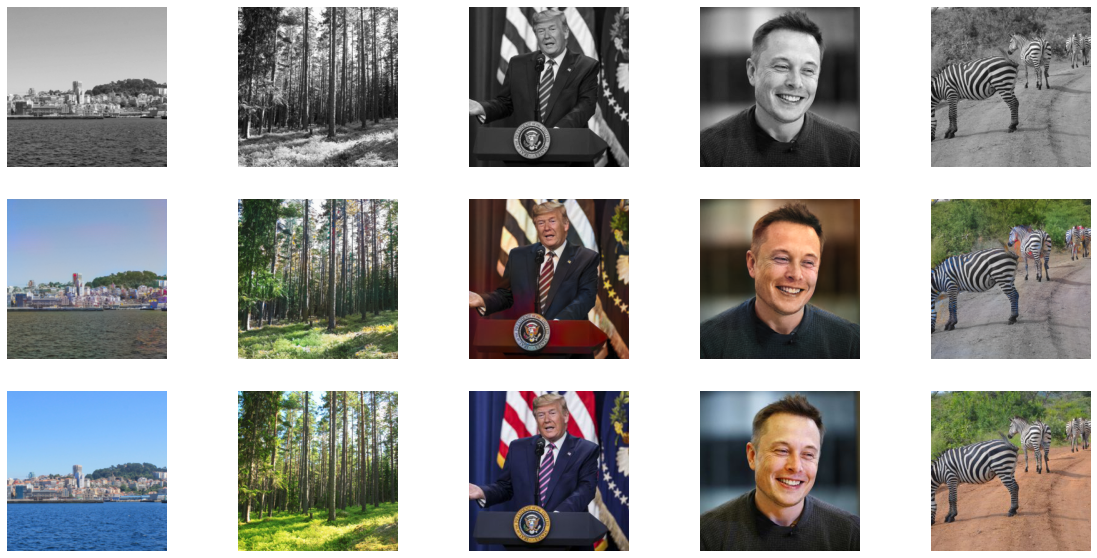
\includegraphics[width=15cm]{images/demo2.png}
\caption{Một số kết quả thử nghiệm khác. Các hàng lần lượt là ảnh xám, ánh sau khi tạo màu, ảnh gốc.}
\label{fig:moreresults}
\end{figure}

\begin{figure}[!h]
\captionsetup{width=0.8\textwidth}
\centering
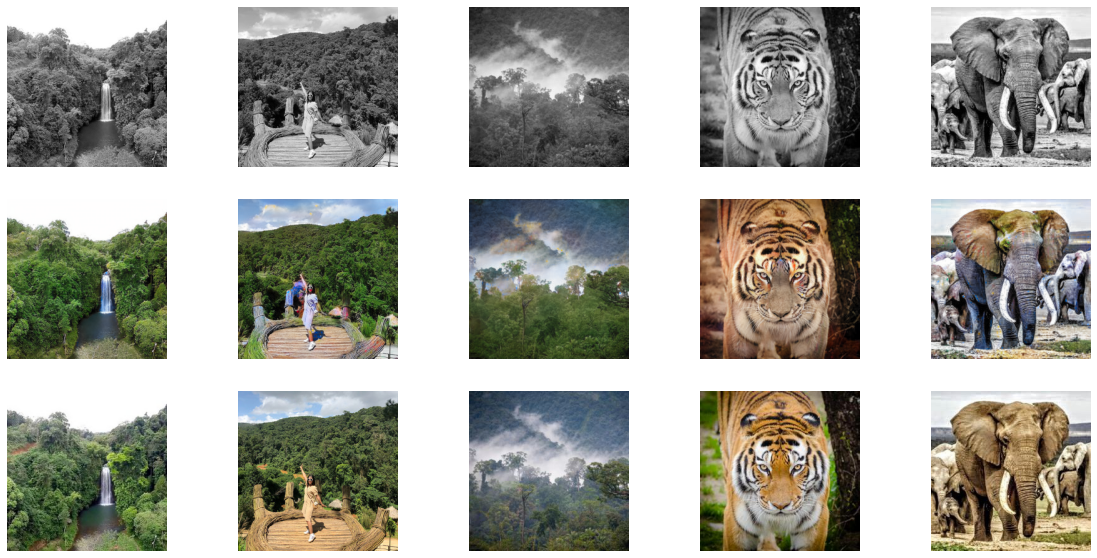
\includegraphics[width=15cm]{images/demo3.png}
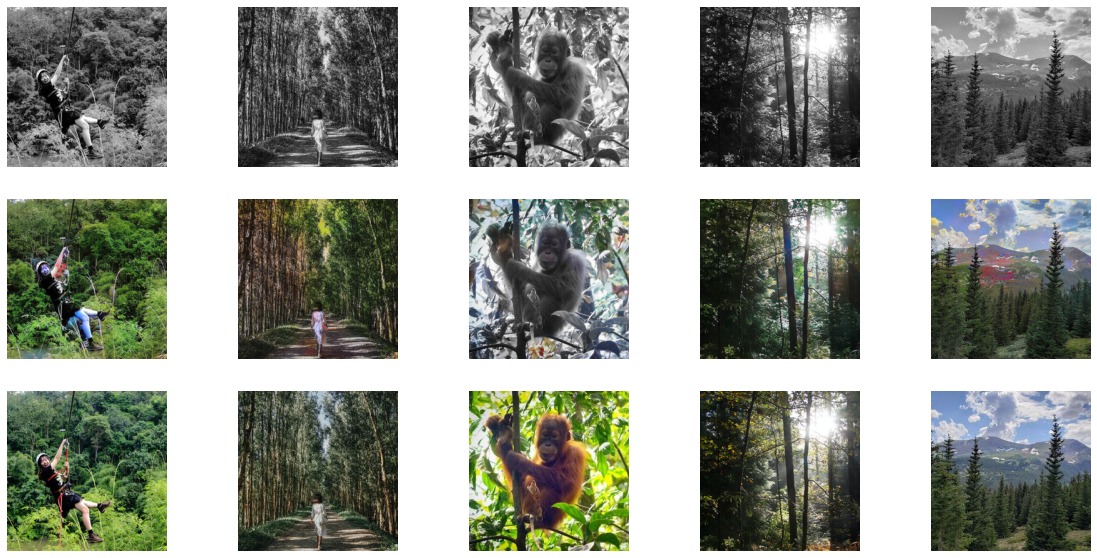
\includegraphics[width=15cm]{images/demo4.png}
\caption{Thêm Một vài kết quả thử nghiệm khác. Các hàng lần lượt là ảnh xám, ánh sau khi tạo màu, ảnh gốc.}
\label{fig:onemoreresults}
\end{figure}

\begin{figure}[!h]
\captionsetup{width=0.8\textwidth}
\centering

\includegraphics[width=14cm]{images/question.PNG}
\caption{Phần mô tả của bài đánh giá.}
\label{fig:dessurvey}
\end{figure}

\begin{figure}[!h]
\captionsetup{width=0.8\textwidth}
\centering
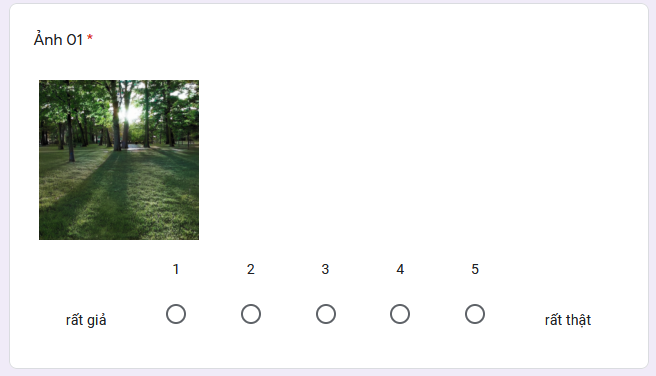
\includegraphics[width=11cm]{images/question2.PNG}
\includegraphics[width=11cm]{images/question3.PNG}
\caption[Phần câu hỏi và số lượng người tham gia cuộc khảo sát thực hiện thông qua Google Forms.]{Phần câu hỏi và số lượng người tham gia cuộc khảo sát thực hiện thông qua Google Forms\protect\footnotemark.}
\label{fig:questionsurvey}
\end{figure}

\begin{figure}[!h]
\captionsetup{width=0.8\textwidth}
\centering
\includegraphics[width=11.8cm]{images/best.PNG}
\caption{Những ảnh có điểm trung bình cao nhất.}
\label{fig:besttests}
\end{figure}

\begin{figure}[!h]
\captionsetup{width=0.8\textwidth}
\centering
\includegraphics[width=11.8cm]{images/worst.PNG}
\caption{Những ảnh có điểm trung bình thấp nhất.}
\label{fig:worsttests}
\end{figure}

\footnotetext{Google Forms, \href{https://www.google.com/forms/about/}{https://www.google.com/forms/about/}}

\begin{table}[h!]
\centering
\begin{tabular}{|c|c|c|c|c|c|c|}
\hline
\diagbox[width=11em]{\textbf{Ảnh}}{\textbf{Thang điểm}}      & \textbf{1} & \textbf{2} & \textbf{3} & \textbf{4} & \textbf{5} & \textbf{Tổng} \\ \hline
\textbf{Ảnh 01}  & 2          & 11         & 29         & \textcolor{JungleGreen}{\textbf{36}}         & 22         & 100         \\ \hline
\textbf{Ảnh 02}  & 20         & \textcolor{Mahogany}{\textbf{35}}         & 24         & 14         & 7          & 100         \\ \hline
\textbf{Ảnh 03}  & 1          & 11         & 21         & 34         & 33         & 100         \\ \hline
\textbf{Ảnh 04}  & 8          & 34         & 30         & 18         & 10         & 100         \\ \hline
\textbf{Ảnh 05}  & 2          & 7          & 18         & 34         & \textcolor{ForestGreen}{\textbf{39}}         & 100         \\ \hline
\textbf{Ảnh 06}  & 9          & 24         & 37         & 21         & 9          & 100         \\ \hline
\textbf{Ảnh 07}  & 1          & 12         & 15         & 34         & 38         & 100         \\ \hline
\textbf{Ảnh 08}  & 1          & 11         & 21         & 35         & 32         & 100         \\ \hline
\textbf{Ảnh 09}  & 1          & 10         & 21         & 30         & 38         & 100         \\ \hline
\textbf{Ảnh 10}  & 8          & 16         & 36         & 29         & 11         & 100         \\ \hline
\textbf{Ảnh 11}  & 4          & 8          & 19         & 33         & 36         & 100         \\ \hline
\textbf{Ảnh 12}  & 2          & 18         & 28         & 26         & 26         & 100         \\ \hline
\textbf{Ảnh 13}  & 7          & 18         & 22         & 34         & 19         & 100         \\ \hline
\textbf{Ảnh 14}  & 6          & 14         & 24         & 34         & 22         & 100         \\ \hline
\textbf{Ảnh 15}  & 13         & 27         & \textcolor{TealBlue}{\textbf{40}}         & 12         & 8          & 100         \\ \hline
\textbf{Ảnh 16}  & 12         & 32         & 23         & 19         & 14         & 100         \\ \hline
\textbf{Ảnh 17}  & 14         & 26         & 30         & 18         & 12         & 100         \\ \hline
\textbf{Ảnh 18}  & 10         & 22         & 26         & 27         & 15         & 100         \\ \hline
\textbf{Ảnh 19}  & 3          & 8          & 23         & 29         & 37         & 100         \\ \hline
\textbf{Ảnh 20}  & \textcolor{red}{\textbf{22}}         & 22         & 26         & 18         & 12         & 100         \\ \hline
\textbf{Tổng}  & 146         & 366         & 513         & \textcolor{Fuchsia}{\textbf{535}}         & 440      & 2000        \\ \hline
\end{tabular}
\caption{Kết quả bình chọn cho các ảnh.}
\label{tab:surveyresults}
\end{table}

\begin{table}[!h]
\centering
\begin{tabular}{c|c|c|c|c|c|}
\cline{2-6}
                                               & \textbf{Ảnh 01} & \textbf{Ảnh 02} & \textbf{Ảnh 03} & \textbf{Ảnh 04} & \textbf{Ảnh 05} \\ \hline
\multicolumn{1}{|c|}{\textbf{Điểm trung bình}} & 3.65            & \textcolor{red}{\textbf{2.53}}            & 3.87            & 2.88            & \textcolor{ForestGreen}{\textbf{4.01}}            \\ \hline
\end{tabular}

\begin{tabular}{c|c|c|c|c|c|}
\cline{2-6}
                                               & \textbf{Ảnh 06} & \textbf{Ảnh 07} & \textbf{Ảnh 08} & \textbf{Ảnh 09} & \textbf{Ảnh 10} \\ \hline
\multicolumn{1}{|c|}{\textbf{Điểm trung bình}} & 2.97            & \textcolor{JungleGreen}{\textbf{3.96}}            & 3.86            & \textcolor{JungleGreen}{\textbf{3.94}}            & 3.19            \\ \hline
\end{tabular}

\begin{tabular}{c|c|c|c|c|c|}
\cline{2-6}
                                               & \textbf{Ảnh 11} & \textbf{Ảnh 12} & \textbf{Ảnh 13} & \textbf{Ảnh 14} & \textbf{Ảnh 15} \\ \hline
\multicolumn{1}{|c|}{\textbf{Điểm trung bình}} & 3.89            & 3.56             & 3.40            & 3.52            & \textcolor{Mahogany}{\textbf{2.75}}            \\ \hline
\end{tabular}

\begin{tabular}{c|c|c|c|c|c|}
\cline{2-6}
                                               & \textbf{Ảnh 16} & \textbf{Ảnh 17} & \textbf{Ảnh 18} & \textbf{Ảnh 19} & \textbf{Ảnh 20} \\ \hline
\multicolumn{1}{|c|}{\textbf{Điểm trung bình}} & 2.91            & 2.88            & 3.15            & 3.89            & \textcolor{Mahogany}{\textbf{2.76}}            \\ \hline
\end{tabular}
\caption{Điểm trung bình của các ảnh.}
\label{tab:statsurvey}
\end{table}

Tuy số lượng mẫu khảo sát nhỏ với chỉ 20 bức ảnh (không đủ làm tổng thể) và sự đa dạng chưa cao, cũng như là số lượng người tham gia khảo sát không quá lớn - chỉ với 100 người.
Nhưng cũng phần nào đánh giá được chất lượng của mô hình.
Nhìn chung, với số điểm trung bình 3.38 và số lượng người đồng tính mức 4 (mức khá) cũng đông đảo nhất với \textbf{535 (26.75\%)} (bảng \ref{tab:surveyresults}) người, thì mô hình có thể xem ở mức \textbf{trung bình--khá}.

\section{So sánh kết quả sau khi huấn luyện lại với tập dữ liệu lớn hơn}\label{enhance_experiments}

\begin{figure}[!h]
\captionsetup{width=0.8\textwidth}
\centering
\includegraphics[width=15cm]{images/enhance.png}
\caption{So sánh thử nghiệm sau khi huấn luyện lại. Hàng thứ 2 là kết quả của mô hình được huấn luyện lại.}
\label{fig:enhance1}
\end{figure}

\begin{figure}[!h]
\captionsetup{width=0.8\textwidth}
\centering
\includegraphics[width=15cm]{images/enhance2.png}
\caption{Thêm một vài so sánh thử nghiệm sau khi huấn luyện lại. Hàng thứ 2 là kết quả của mô hình được huấn luyện lại.}
\label{fig:enhance2}
\end{figure}

Đây là mô hình được khởi tạo theo kiến trúc và các thông số hoàn toàn giống với mô hình mà ta đã thử nghiệm [\textbf{\ref{surveyforevaluation}}].
Mô hình được huấn luyện qua 15 epoch với một tập dữ liệu giàu hơn, gồm $18,000$ bức hình (so với $10,000$ của mô hình cũ) từ tập dữ liệu COCO.
Số lượng đã tăng gấp 1.8 lần, kết hợp phương pháp làm giàu dữ liệu thì số lượng gấp 3.6 lần.\vspace{5pt}

Việc huấn luyện với số lượng dữ liệu nhiều hơn, giúp cho mô hình có thêm nhiều hiểu biết về các đặc trưng.
Từ đó, một số kết quả trở nên chân thực hơn (hình \ref{fig:enhance1}, cột 2; hình \ref{fig:enhance2}, cột 3).\vspace{5pt}

Một sự khác biệt ở mô hình này, là quá trình huấn luyện không qua bước tiền huấn luyện bộ sinh.
Có lẽ cũng vì vậy, mà màu của mô hình này tươi sáng hơn rất nhiều, khi có nhiều điểm ảnh được cho màu đỏ hoặc lam (màu áo ở hình \ref{fig:enhance1}, cột thứ 5).
Việc dũng cảm hơn trong việc tô màu, thay vì chọn màu xám, giúp cho một vài thứ có kết quả đẹp hơn (màu đèn ở hình \ref{fig:enhance1}, cột thứ 4; màu nước ở hình \ref{fig:enhance2}, cột thứ 4).
Nhưng cũng đầy rủi ro, khi lại dễ dàng gây ra sự lem luốc (màu trời, màu toà nhà hình \ref{fig:enhance2}, cột thứ 5).
Cũng giống với vua Midas, ta cần phải hiểu rõ cái ta muốn.
Để cân đối được chuyện sáng tạo cho mô hình, công việc này cần thêm nhiều thử nghiệm trong tương lai.

\section{Đánh giá định lượng hai mô hình trước và sau khi cải thiện bằng MSE và RMSE}\label{mseandrmseeval}

Mô hình trước cải thiện $\mathcal{G}_1$ là mô hình được huấn luyện với $10,000$ ảnh.
Sau cải thiện là mô hình $\mathcal{G}_2$ được huấn luyện với $18,000$ ảnh.
Ta sẽ đánh giá hai mô hình qua MSE \cite{wikimse2021} và RMSE \cite{wikirmse2021}.
Công thức để đánh giá MSE sử dụng được cho ở (\ref{eqn:mse}), còn RMSE là căn bậc 2 của MSE (\ref{eqn:rmse}).\vspace{5pt}

Ta sẽ khảo sát 2 ảnh kênh màu, tức là $\widehat{\mathcal{I}}_{\text{đầu ra } \mathcal{G}_1} = \mathcal{G}_1\left(\mathcal{I}_{\text{đầu vào}}\right)$ với $\widehat{\mathcal{I}}_{\text{đầu ra } \mathcal{G}_2} = \mathcal{G}_2\left(\mathcal{I}_{\text{đầu vào}}\right)$ so với $\mathcal{I}_{\text{đầu ra}}$.
Ở đây, $\mathcal{I}_{\text{đầu ra}}, \mathcal{I}_{\text{đầu ra } \mathcal{G}_1}, \mathcal{I}_{\text{đầu ra } \mathcal{G}_2}$ sẽ được chuẩn hoá theo tập $[-110, 110] \times [-110, 110]$.
\begin{align}
    \text{MSE} = \frac{2}{256\times 256}\sum_{k=1}^{2}\sum_{i=1}^{256}\sum_{j=1}^{256}\left\{\widehat{\mathcal{I}}_{\text{đầu ra}} - \mathcal{I}_{\text{đầu ra}}\right\}^2 \label{eqn:mse}\\
    \text{RMSE} = \sqrt{\text{MSE}} = \sqrt{\frac{2}{256\times 256}\sum_{k=1}^{2}\sum_{i=1}^{256}\sum_{j=1}^{256}\left\{\widehat{\mathcal{I}}_{\text{đầu ra}} - \mathcal{I}_{\text{đầu ra}}\right\}^2} \label{eqn:rmse}
\end{align}

\begin{table}[!h]
\centering
\begin{tabular}{c|c|c|c|c|}
\cline{2-5}
                                    & \textbf{Ảnh 02 (\textcolor{red}{\textbf{2.53}})}  & \textbf{Ảnh 07 (\textcolor{JungleGreen}{\textbf{3.96}})}  & \textbf{Ảnh 09 (\textcolor{JungleGreen}{\textbf{3.94}})}  & \textbf{Ảnh 15 (\textcolor{Mahogany}{\textbf{2.75}})}  \\ \hline
\multicolumn{1}{|c|}{\textbf{MSE} $\mathcal{G}_1$}  & 374.2613         & 312.994          & \textcolor{ForestGreen}{\textbf{240.9714}}         & 628.1626         \\ \hline
\multicolumn{1}{|c|}{\textbf{MSE} $\mathcal{G}_2$}  & 409.466          & 202.8153         & \textcolor{ForestGreen}{\textbf{150.6662}}         & 442.2453         \\ \hline
\multicolumn{1}{|c|}{\textbf{RMSE} $\mathcal{G}_1$} & 19.3458          & 17.6916          & \textcolor{ForestGreen}{\textbf{15.5233}}          & 25.0632          \\ \hline
\multicolumn{1}{|c|}{\textbf{RMSE} $\mathcal{G}_2$} & 20.2353          & 14.2413          & \textcolor{ForestGreen}{\textbf{12.2746}}          & 21.0296          \\ \hline
\end{tabular}
\caption{Kết quả MSE và RMSE của hai mô hình trên 4 ảnh được chọn.}
\label{tab:msermse}
\end{table}

Có 4 ảnh được đem ra để đánh giá.
Trong đó, một nửa là 2 tấm trong những ảnh có kết quả tệ (ảnh 02, ảnh 15), còn lại là 2 tấm trong nhóm kết quả tốt (ảnh 07, ảnh 09) [\textbf{\ref{surveyforevaluation}}].
Kết quả được cho ở bảng \ref{tab:msermse}.\vspace{5pt}

Một điều dễ thấy đó là, mô hình $\mathcal{G}_2$ cho kết quả tốt hơn so với $\mathcal{G}_1$ khi 3/4 ảnh (ảnh 07, ảnh 09 và ảnh 15) có kết quả MSE thấp hơn.
Ảnh 02 là một ảnh nhiều chi tiết, với tính cách tinh nghịch của $\mathcal{G}_2$ khi không được tiền huấn luyện, rất dễ để có những màu lệch so với màu gốc.
Nên MSE của $\mathcal{G}_2$ cao hơn so với của $\mathcal{G}_1$.\vspace{5pt}

Thông qua RMSE, ta có thể thấy được rằng, mỗi điểm màu của cả hai mô hình sẽ chệnh lệch khoảng 10 đến 20 (thấp nhất là 12.2746 của $\mathcal{G}_2$ với ảnh 09, nhiều nhất là 25.0632 của $\mathcal{G}_1$ với ảnh 15) đơn vị so với ảnh gốc.
Kết quả này quả thực không quá tệ khi chỉ chênh khoảng $100\% \times \dfrac{10}{2\times 110} = 4.55 \%$ đến $100\% \times \dfrac{20}{2\times 110} = 9.09 \%$ so với khoảng giá trị.


%%%%%%%%%%%%%%%%%%%%%%%%%%%%%%%%%
\chapter{Ứng dụng}

\section{Giao diện lập trình ứng dụng (API - Application Programming Interface) bằng khung phần mềm Django của Python}

Để có thể dễ dàng chia sẻ tính năng phần mềm, cụ thể là việc tạo màu, API là một phương thức hữu hiệu được sử dụng nhiều nhất hiện nay.
Ngoài ra, với việc mô hình được triển khai bằng ngôn ngữ Python, một ngôn ngữ có một khung phần mềm lập trình liên quan về website mạnh mẽ như Django, là một lợi thế.\vspace{5pt}

Dựa trên những cơ sở đó, một API tạo màu đã được xây dựng có endpoint là \href{domain/main/}{domain/main/} (trong quá trình thử nghiệm, \texttt{domain} là \texttt{localhost:8000}).
Phương thức gửi yêu cầu được chấp nhận là \textbf{POST}.
Nội dung ảnh sẽ được đính kèm, không qua mã hoá, trong phần thân của yêu cầu gửi tới (hình \ref{fig:demoinpostman}).
Vì mục đích thử nghiệm là chủ yếu, các phương thức bảo mật CSRF, CORS (hình \ref{fig:cors}) được tắt để tránh gây phiền hà khi thao tác.

\begin{figure}[!h]
\centering
\includegraphics[width=16cm]{images/cors.png}
\caption{Bảo mật CORS cản trở khi thử nghiệm API}
\label{fig:cors}
\end{figure}

\begin{figure}[!h]
\centering
\includegraphics[width=16cm]{images/readablestream.png}
\caption{Phản hồi trả về của endpoint}
\label{fig:readablestreamresponse}
\end{figure}

Khi nhận được yêu cầu, endpoint tiếp nhận và xử lý, sau đó trả về phản hồi đính kèm ảnh được tạo màu dưới định dạng dữ liệu ReadableStream (hình \ref{fig:readablestreamresponse}).

\begin{figure}[!h]
\centering
\includegraphics[width=15cm]{images/postman.png}
\caption{Thử nghiệm API trên phần mềm Postman}
\label{fig:demoinpostman}
\end{figure}

\section{Ứng dụng web với khung phần mềm VueJS của Javascript và API}

Tận dụng API đã được xây dựng, kết hợp với khung phần mềm thiết kế giao diện VueJS, ta dễ dàng tạo được một ứng dụng website thân thiện với người dùng (hình \ref{fig:webapp}).
Chỉ cần chọn một tấm ảnh xám, ứng dụng trả về một tấm ảnh sau khi được tạo màu và cho phép người dùng tải về.

\begin{figure}[!h]
\centering
\includegraphics[width=15cm]{images/demoweb.png}
\caption{Ứng dụng web tạo màu đơn giản bằng VueJS kết hợp API}
\label{fig:webapp}
\end{figure}

%%%%%%%%%%%%%%%%%%%%%%%%%%%%%%%%%
\chapter{Tổng kết}

\section{Kết luận}

Một phương pháp tạo màu cho ảnh xám đã được trình bày thông qua đồ án này.
Phương pháp sử dụng khung mô hình một mạng đối nghịch tạo sinh có điều kiện - cGAN theo khung mô hình pix2pix.
Mạng gồm bộ phân biệt kiến trúc Patch $70 \times 70$, và một bộ sinh mạng tích chập kiến trúc Unet có phần xương sống học chuyển giao từ mạng tích chập ResNet18.\vspace{5pt}

Mô hình được lập trình và huấn luyện bằng ngôn ngữ Python, trên nên tảng mã nguồn mở về máy học Pytorch của Facebook's AI Research lab.
Quá trình huấn luyện cho ra hai mô hình.
Mô hình đầu tiên được huấn luyện theo hàm mất mát kiểu GAN kết hợp với một hàm mất mát truyền thống chuẩn 1, trên tập dữ liệu 10,000 bức ảnh của COCO (kết hợp với làm giàu dữ liệu là 20,000 bức ảnh).
Mô hình thứ hai là mô hình cải thiện với các thông số khởi tạo giống với mô hình ban đầu, nhưng hàm mất mát không còn kết hợp hàm mất mát chuẩn 1.
Tập dữ liệu cũng được mở rộng hơn với 18,000 bức ảnh của COCO (kết hợp với làm giàu dữ liệu là 36,000 bức ảnh).\vspace{5pt}

Chất lượng mô hình đầu tiên được đánh giá dựa qua một cuộc khảo sát thực tế, với sự tham gia giúp đỡ của 100 người.
Bài khảo sát bao gồm 20 bức ảnh có màu tạo từ bộ sinh, theo thang điểm từ 1 (rất giả) tới 5 (rất thật).
Kết quả nhận được là số điểm trung bình 3.38, trong đó số điểm cao nhất là 4.01 và thấp nhất là 2.53.
Sau khi cải thiện mô hình, kết quả MSE và RMSE đã cho thấy mô hình sau đã được cải thiện hơn so với mô hình trước.
Theo như mục tiêu được đề ra, cả hai mô hình đã hoàn thành được ở mức trung bình--khá cho tới khá.\vspace{5pt}

Bên cạnh đó, cũng đã thành công xây dựng một API tạo màu bằng khung phần mềm Django của Python.
Từ đó triển khai một ứng dụng web đơn giản để tạo màu cho ảnh bằng khung phần mềm VueJS của Javascript.\vspace{5pt}

\textbf{Đề tài của đồ án đã được hoàn thành.}

\section{Hạn chế và hướng cải thiện mô hình}\label{enhancemodel}

Mô hình vẫn chưa có kết quả tốt khi áp dụng với những ảnh có một số đặc trưng lạ, những đặc trưng chưa được học trong quá trình huấn luyện.
Để cải thiện trí tuệ mô hình, ta cần tìm thêm nhiều tập dữ liệu với các đối tượng, đặc trưng phong phú để huấn luyện thêm.
Ngoài ra, sử dụng một xương sống tốt hơn mạng ResNet18 hiện có, chẳng hạn ResNet34, ResNet50, ResNet101, hoặc một họ mạng khác như VGG hay Xception.\vspace{5pt}

Một cách tiếp cận khác để cải thiện mô hình, đó là huấn luyện nhiều bộ sinh.
Mỗi bộ sinh sẽ đảm nhiệm một nhóm đặc trưng nhất định.
Như vậy chỉ cần cho bộ sinh học những ảnh liên quan đến chủ đề của mình.
Bằng việc chuyên môn hoá chủ đề cho bộ sinh, ta không còn yêu cầu một bộ sinh có thể tạo màu tốt với mọi ảnh đầu vào.
Thay vào đó, cho kết quả tốt hơn cả khi được đưa cho ảnh đúng chuyên môn.
Quá trình huấn luyện cũng được đơn giản hơn do mô hình không phải học quá nhiều.\vspace{5pt}

Một số những đề xuất về việc sử dụng GAN để tạo màu có kết quả tốt có thêm tham khảo thêm như \cite{Nazeri_2018}, khi tác giả sử dụng mạng GAN tích chập sâu - DCGAN áp dụng với ảnh độ phân giải cao, tăng tốc độ và ổn định huấn luyện.
Cao và các cộng sự của mình \cite{cao2017unsupervised} cũng sử dụng cGAN để tạo màu một cách đa dạng nhờ vào lấy mẫu nhiễu đầu vào nhiều lần.
Một đột phá khác, Vitoria \cite{vitoria2020chromagan} nhận thấy rằng ta có tận dụng phân phối phân lớp trong quá trình huấn luyện cho mạng GAN, và đưa ra mô hình với cái tên là ChromaGAN.

\section{Hướng phát triển đề tài}

Đề tài có thể được áp dụng để làm những tác vụ liên quan đến phục chế màu cho ảnh xám, bị mất màu hoặc ảnh cũ xưa, thời chiến tranh.
Giúp cho quá trình phục chế được tiết kiệm thời gian.
Phối hợp với một ít tinh chỉnh bằng phương pháp thủ công, ta hoàn toàn có thể có những kết quả phục chế đẹp đẽ và tiết kiệm được rất nhiều thời gian.\vspace{5pt}

Không chỉ dừng lại ở hình ảnh đơn lẻ, ta cũng có thể áp dụng mô hình để phục chế màu cho các video, vì bản chất một video là sự kết hợp từ nhiều khung hình ghép lại.
Trong thư mục đồ án, phần \texttt{test\_results} có một kết quả thử nghiệm của mô hình đầu tiên trong việc phục chế màu một đoạn nhỏ về phóng sự về chiến tranh ở Việt Nam.

\begin{figure}[!h]
\captionsetup{width=0.85\textwidth}
\centering
\includegraphics[width=15cm]{images/final.PNG}
\caption{Ảnh Trường ĐH Bách Khoa TP.HCM ngày xưa khi chưa có màu (trên) và sau khi tô màu: mô hình ban đầu (trái), mô hình sau khi cải thiện (phải)}
\label{fig:bkhcmold}
\end{figure}

\renewcommand{\bibname}{Tài liệu tham khảo}
%%%%%%%%%%%%%%%%%%%%%%%%%%%%%%%%%
\printbibliography

\end{document}